\documentclass[11pt,a4paper]{article}
\usepackage[utf8]{inputenc}
\usepackage[T1]{fontenc}
\IfFileExists{spanish.ldf}{\usepackage[spanish,es-nodecimaldot]{babel}}{\usepackage[provide=*,main=spanish]{babel}}
\usepackage[margin=2.2cm]{geometry}
\usepackage{amsmath,amssymb,booktabs,longtable,tabularx,array}
\usepackage{enumitem,xcolor,hyperref,xurl,tikz}
\usetikzlibrary{arrows.meta,positioning}
\hypersetup{colorlinks=true,linkcolor=blue!55!black,urlcolor=blue!55!black,
  pdftitle={TerraPulse AI: documentación técnica del proyecto},
  pdfauthor={Equipo TerraPulse AI}}
\setlist{leftmargin=*,itemsep=3pt}
\setlength{\parskip}{5pt}
\setlength{\emergencystretch}{1.5em}
\setcounter{tocdepth}{2}
\usepackage{graphicx}
\graphicspath{{fig/}}
\usepackage{caption}
\captionsetup{font=small,labelfont=bf,margin=0.6cm}
\usepackage[skins,breakable]{tcolorbox}
\tcbset{boxrule=0.6pt,arc=2pt,left=6pt,right=6pt,top=4pt,bottom=4pt,fonttitle=\bfseries\small,before skip=8pt,after skip=8pt}
\newtcolorbox{intuicion}{colback=blue!4,colframe=blue!55!black,title={Intuición},breakable}
\newtcolorbox{cuidado}{colback=orange!8,colframe=orange!75!black,title={Cuidado},breakable}
\newtcolorbox{atencion}{colback=orange!8,colframe=orange!75!black,title={Atención},breakable}
\newtcolorbox{ejemplo}[1][Ejemplo]{colback=green!5,colframe=green!45!black,title={#1},breakable}
\newcommand{\figura}[3]{%
  \begin{figure}[htbp]\centering
    \IfFileExists{fig/#1.pdf}{%
      \includegraphics[width=#2\linewidth]{fig/#1.pdf}%
    }{%
      \fbox{\begin{minipage}{#2\linewidth}
        \centering\vspace{2.5cm}
        \textit{Figura pendiente: \detokenize{#1}}\\
        \small Recurso gráfico no incluido en el proyecto.
        \vspace{2.5cm}
      \end{minipage}}%
    }
    \caption{#3}\label{fig:#1}
  \end{figure}%
}


% --- macros comunes
\newcommand{\src}[1]{\nolinkurl{#1}}
\newcommand{\dd}{\mathrm d}
\newcommand{\unit}[1]{\mathrm{#1}}
\newcommand{\warn}[1]{\par\noindent\colorbox{blue!8}{\parbox{.965\linewidth}{\textbf{Lectura crítica.} #1}}\par}
% --- macros de la Parte II (radar)
\newcommand{\gz}{\ensuremath{\gamma^{0}}}
\newcommand{\sz}{\ensuremath{\sigma^{0}}}
\newcommand{\por}{\ensuremath{\times}}
\newcommand{\flecha}{\ensuremath{\rightarrow}}
\pdfstringdefDisableCommands{\def\gz{gamma0}\def\sz{sigma0}\def\por{x}\def\flecha{->}}

% --- \part compacto: sin página propia
\makeatletter
\renewcommand\part{\if@noskipsec \leavevmode \fi \par \addvspace{4ex}\@afterindentfalse \secdef\@part\@spart}
\def\@part[#1]#2{%
  \refstepcounter{part}%
  \addcontentsline{toc}{part}{\partname~\thepart\hspace{0.6em}#1}%
  {\parindent\z@ \raggedright \interlinepenalty\@M \normalfont
   \Large\bfseries \partname\nobreakspace\thepart \par\nobreak
   \Huge\bfseries #2\markboth{}{}\par}%
  \nobreak \vskip 3ex \@afterheading}
\makeatother

\title{TerraPulse AI\\[4pt]\Large El pulso cambiante de nuestro planeta\\[6pt]\large Documentación técnica del proyecto\\[2pt]\normalsize Reto: Bailando con los SARs}
\author{Equipo TerraPulse AI}
\date{15 de noviembre de 2026}
\begin{document}

\maketitle
\tableofcontents
\listoffigures
\listoftables
\newpage

\part{El proyecto}
\label{part:proyecto}

\section{Resumen del proyecto}
\label{sec:resumen}

TerraPulse AI («El pulso cambiante de nuestro planeta») es una plataforma web abierta que convierte
observaciones de radar de la misión NASA--ISRO NISAR en evidencia geoespacial comprensible y reproducible.
No es solo un visor de imágenes. Arma una cadena trazable completa: consulta el catálogo de ASF, revisa que
las escenas sean comparables (trayectoria, marco, polarización, versión de procesamiento y madurez), recorta
los productos GCOV a la región de interés y calcula el cambio en la retrodispersión entre dos fechas
($\Delta\sigma^0$ en dB). Después contrasta ese cambio con fuentes independientes como la precipitación de
GPM IMERG, imágenes ópticas HLS o los productos OPERA.

Para el reto \emph{Bailando con los SARs}, el proyecto estudia Chiapas, México, con un par de escenas NISAR
comparables de junio a octubre de 2026. Cada cifra se puede rastrear hasta la escena, la fecha, los
parámetros y el código que la produjeron. El proyecto distingue entre observación, inferencia y predicción, y
no atribuye causas que el radar no puede demostrar por sí solo.

Es importante porque el radar ve de día y de noche, y también a través de las nubes, algo clave en regiones
tropicales. Además, permite que investigadores, autoridades y comunidades tomen decisiones con datos
verificables.

\section{Descripción detallada}
\label{sec:detalle}

\subsection{¿Qué hace y cómo funciona?}

TerraPulse AI lleva datos públicos de radar NISAR (banda L) desde el archivo original hasta un mapa
interactivo, sin perder el rastro de dónde viene cada valor. El flujo tiene cinco pasos:
\begin{enumerate}
  \item \textbf{Catálogo.} Consulta ASF y agrupa los productos GCOV en pilas que se pueden comparar entre
        sí. Para eso deben coincidir en trayectoria, marco, dirección, polarización, versión de
        procesamiento (CRID) y madurez.
  \item \textbf{Control de comparabilidad.} Rechaza los pares que no se deben mezclar, por ejemplo BETA con
        PROVISIONAL o dos CRID distintos.
  \item \textbf{Recorte inteligente.} Cada escena pesa unos 7\,GB. En lugar de descargarla completa, se
        leen por HTTPS solo los bloques del archivo \texttt{.h5} que caen dentro de la región de interés.
        Luego se verifican la identidad de la escena, la cobertura real (99.6\,\% de píxeles válidos en el
        par de Chiapas) y que la malla sea idéntica en las dos fechas.
  \item \textbf{Inspección y exportación web.} Genera rasters optimizados para la nube (COG), capas para el
        mapa y gráficas, todo con sus metadatos.
  \item \textbf{Plataforma web.} Muestra las capas SAR en un mapa, un comparador antes/después con cortina
        deslizable, gráficas y paneles de métricas.
\end{enumerate}
Además, el proyecto incluye dos simuladores exploratorios sobre el relieve real de NASADEM:
\begin{itemize}
  \item \textbf{Inundación:} usa el modelo hidrodinámico LISFLOOD-FP con escenarios de lluvia
        (Parte~\ref{part:inundacion}).
  \item \textbf{Radiación solar sobre el terreno:} calcula la posición del sol y la irradiancia de cielo
        despejado para una ROI y una hora elegidas (Parte~\ref{part:solar}).
\end{itemize}
Ambos se presentan como modelos sin validar, nunca como observaciones.

\subsection{Beneficios e impacto}

El radar ve de noche y a través de las nubes, algo decisivo en Chiapas, donde la nubosidad limita a los
satélites ópticos. TerraPulse permite que investigadores, autoridades de protección civil, estudiantes y
comunidades exploren cambios en la superficie con datos verificables. También explica qué significa cada
métrica y qué no significa. Como el flujo es abierto y reproducible, cualquiera puede repetirlo en otra
región.

\subsection{Herramientas utilizadas}

\begin{itemize}
  \item \textbf{Lenguajes:} Python 3.11, TypeScript, SQL.
  \item \textbf{Datos:} NISAR GCOV (ASF Vertex / NASA Earthdata) y NASADEM. Las fuentes auxiliares de
        validación son GPM IMERG, HLS y OPERA.
  \item \textbf{Procesamiento:} h5py, rasterio, GDAL, xarray, rioxarray, geopandas, numpy, asf\_search,
        earthaccess, LISFLOOD-FP y pvlib.
  \item \textbf{Backend:} Django, GeoDjango, Django REST Framework, PostgreSQL + PostGIS, Celery + Redis.
  \item \textbf{Frontend:} React, Vite, MapLibre GL, Chart.js.
  \item \textbf{Infraestructura:} Docker y Docker Compose, con pruebas en pytest. El desarrollo se hace en
        computadoras personales.
\end{itemize}

\section{Contexto: ¿por qué un radar para observar cambios en la superficie?}
\label{sec:contexto}

Observar la superficie de la Tierra de forma repetida es la base de casi cualquier pregunta sobre cambio:
cuánta agua cubre un terreno después de una tormenta, cómo evoluciona la vegetación a lo largo del año, si un
suelo se humedeció o se secó entre dos fechas. Los satélites ópticos (los que producen imágenes parecidas a
una fotografía) responden bien a esas preguntas cuando el cielo está despejado y hay luz solar. En una región
tropical como Chiapas, donde la nubosidad es frecuente durante la temporada de lluvias, esa condición se
cumple con menos regularidad justamente cuando más interesa mirar.

Un radar de apertura sintética (SAR, por \emph{Synthetic Aperture Radar}) funciona de otra manera. En vez de
registrar la luz solar reflejada, el propio satélite emite pulsos de microondas hacia la superficie y mide el
eco que regresa. Por eso:
\begin{itemize}
  \item \textbf{No depende de la luz del día:} la fuente de iluminación es el radar, así que puede observar
        de noche.
  \item \textbf{Atraviesa las nubes:} a las longitudes de onda de microondas, las nubes y la lluvia ligera
        casi no interfieren.
  \item \textbf{Mide propiedades distintas a las del color:} lo que importa es la forma, la rugosidad y la
        humedad de lo que refleja, no su aspecto visual.
\end{itemize}
La misión NISAR, desarrollada conjuntamente por la NASA y la agencia espacial india ISRO, lleva radares en
banda L y en banda S. TerraPulse AI usa la \textbf{banda L} (longitud de onda cercana a 24\,cm), que penetra el
follaje mejor que las bandas más cortas y responde a estructuras grandes de la vegetación y a la humedad del
suelo. Los productos que se usan son los GCOV (\emph{Geocoded Polarimetric Covariance}), que ya vienen
proyectados sobre una malla de mapa.

\begin{intuicion}
Una imagen de radar \emph{no} es una fotografía en blanco y negro. Cada píxel es una medida de cuánta energía
de microondas regresó al satélite desde ese lugar. Un píxel oscuro puede ser agua en calma (que refleja la
señal lejos del satélite) o una ladera que le da la espalda al radar; uno brillante puede ser un techo, un
tronco rodeado de agua o simple suerte estadística (el \emph{moteado}). Leer una imagen SAR consiste en
entender qué mecanismo físico produjo cada nivel de brillo.
\end{intuicion}

\section{La cadena de datos de punta a punta}
\label{sec:cadena}

TerraPulse AI no es una sola herramienta, sino una cadena en la que cada eslabón recibe algo verificado del
anterior y entrega algo verificable al siguiente. La figura~\ref{fig:cadena-datos} resume el recorrido, y la
tabla~\ref{tab:eslabones} detalla qué entra, qué sale y qué se comprueba en cada paso.

\begin{figure}[htbp]
\centering
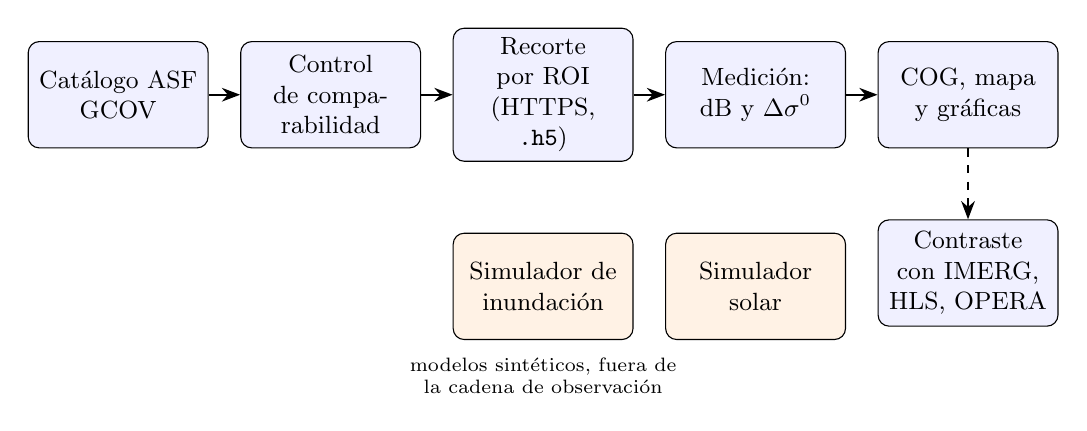
\begin{tikzpicture}[node distance=4mm,
  caja/.style={draw,rounded corners,fill=blue!6,align=center,text width=2.05cm,minimum height=1.35cm,font=\small},
  mod/.style={caja,fill=orange!10},
  fl/.style={-{Stealth},thick}]
\node[caja] (a) {Catálogo ASF\\GCOV};
\node[caja,right=of a] (b) {Control de comparabilidad};
\node[caja,right=of b] (c) {Recorte por ROI (HTTPS, \texttt{.h5})};
\node[caja,right=of c] (d) {Medición: dB y $\Delta\sigma^0$};
\node[caja,right=of d] (e) {COG, mapa y gráficas};
\node[mod,below=9mm of c] (f) {Simulador de inundación};
\node[mod,right=of f] (g) {Simulador solar};
\node[caja,below=9mm of e] (h) {Contraste con IMERG, HLS, OPERA};
\draw[fl] (a)--(b); \draw[fl] (b)--(c); \draw[fl] (c)--(d); \draw[fl] (d)--(e);
\draw[fl,dashed] (e)--(h);
\node[font=\scriptsize,below=1mm of f,text width=4.3cm,align=center] {modelos sintéticos, fuera de la cadena de observación};
\end{tikzpicture}
\caption{La cadena de observación (arriba) y los dos simuladores exploratorios (abajo, en naranja). Los
simuladores comparten el relieve de NASADEM pero no alimentan ni validan las mediciones de radar.}
\label{fig:cadena-datos}
\end{figure}

\begin{table}[htbp]
\centering\small
\begin{tabularx}{\linewidth}{p{.19\linewidth}p{.24\linewidth}p{.22\linewidth}X}
\toprule
\textbf{Eslabón} & \textbf{Entra} & \textbf{Sale} & \textbf{Qué se comprueba}\\\midrule
Catálogo & Consulta a ASF & Pilas de productos GCOV & Que los metadatos describan la misma trayectoria y marco\\
Comparabilidad & Pilas candidatas & Pares aceptados o rechazados & Misma trayectoria, marco, dirección, polarización, CRID y madurez\\
Recorte & Escena de $\approx$7\,GB, ROI & Bloques de la ROI & Identidad de la escena, cobertura válida y malla idéntica en ambas fechas\\
Medición & Potencia \gz{} y máscara & dB, multilook, $\Delta\sigma^0_{dB}$ & Píxeles válidos, escala común, estadísticas reproducibles\\
Exportación & Rasters de la medición & COG, capas, gráficas & Metadatos y hashes que ligan cada capa a su escena\\
Contraste & Mapas de cambio & Evidencia independiente & Coherencia con precipitación, imágenes ópticas y productos OPERA\\\bottomrule
\end{tabularx}
\caption{Qué entra, qué sale y qué se comprueba en cada eslabón de la cadena de observación.}
\label{tab:eslabones}
\end{table}

\paragraph{Por qué el orden importa.} El control de comparabilidad ocurre \emph{antes} de gastar ancho de banda
en el recorte y mucho antes de calcular un cambio. Un par de escenas con distinta versión de procesamiento
(CRID) o distinta madurez (por ejemplo BETA frente a PROVISIONAL) puede mostrar diferencias que no vienen de
la superficie sino del propio procesamiento. Rechazar esos pares al principio es más barato y más honesto que
explicar después un cambio espurio.

\section{Observación, inferencia y predicción}
\label{sec:tres-niveles}

Una regla atraviesa todo el proyecto: cada afirmación se etiqueta según de dónde viene. La
tabla~\ref{tab:niveles} resume los tres niveles y cómo se tratan en este documento.

\begin{table}[htbp]
\centering\small
\begin{tabularx}{\linewidth}{p{.17\linewidth}p{.36\linewidth}X}
\toprule
\textbf{Nivel} & \textbf{Qué es} & \textbf{Ejemplo en este documento}\\\midrule
Observación & Un número leído o calculado directamente del producto, con su rastro hasta el archivo. &
La media de $\gamma^0_{HH}$ en la ROI es $-8.055$\,dB (Parte~\ref{part:radar}).\\
Inferencia & Una explicación plausible que no se ha verificado con datos independientes. &
La brecha de 4.3\,dB entre la media lineal y la media en dB \emph{probablemente} refleja coberturas mezcladas y píxeles muy brillantes.\\
Predicción / escenario & Resultado de un modelo con supuestos declarados. &
Una profundidad de agua simulada con lluvia sintética (Parte~\ref{part:inundacion}); una irradiancia de cielo despejado (Parte~\ref{part:solar}).\\\bottomrule
\end{tabularx}
\caption{Los tres niveles de afirmación y cómo se distinguen.}
\label{tab:niveles}
\end{table}

Los dos simuladores pertenecen siempre al tercer nivel. Que el servicio devuelva un mapa bien formado,
descargable y con los metadatos correctos demuestra que la \emph{integración técnica} funciona; no demuestra
que el mapa describa un evento real. Esa distinción se repite deliberadamente en las Partes
\ref{part:inundacion} y~\ref{part:solar}.

\section{Cómo está pensada la lectura de este documento}
\label{sec:como-leer}

El documento se puede leer en tres capas, y las tres conviven en cada parte:
\begin{enumerate}
  \item \textbf{Intuición.} Recuadros azules y figuras que explican, sin fórmulas, qué hace una ecuación y por
        qué existe.
  \item \textbf{Ecuación.} La expresión matemática con todas sus magnitudes y unidades, y una comprobación
        dimensional cuando ayuda.
  \item \textbf{Ejemplo y código.} Recuadros verdes con un cálculo resuelto paso a paso y referencias a las
        funciones del repositorio que implementan la idea.
\end{enumerate}
Hay además recuadros naranjas de \textbf{cuidado}, que marcan interpretaciones que parecen razonables pero no
están justificadas. Los ejemplos numéricos que no provienen de una escena real están rotulados como
\emph{ilustrativos}; las cifras que sí provienen del producto de la Etapa 1 se identifican como tales.

\section{Organización de este documento}
\label{sec:organizacion}

Este documento reúne la documentación técnica del proyecto en nueve partes:
\begin{description}[style=nextline]
  \item[Parte~\ref{part:proyecto}. El proyecto.] Qué es TerraPulse AI, por qué usa radar, cómo fluye un dato
        de punta a punta y cómo se separa lo observado de lo supuesto.
  \item[Parte~\ref{part:fundamentos}. Fundamentos del radar de apertura sintética.] Qué mide un SAR, qué es el
        moteado y qué contiene un producto GCOV. Es la base conceptual de las ecuaciones.
  \item[Parte~\ref{part:radar}. Ecuaciones del radar.] La medición, el cambio entre fechas y su interpretación;
        qué ecuación produce cada figura de la Etapa 1, con explicaciones y figuras de apoyo.
  \item[Parte~\ref{part:pixel}. Del píxel al análisis.] El recorrido de un píxel, de la lectura a la
        estadística regional, con ejemplos numéricos y la lista de comprobación antes de interpretar.
  \item[Parte~\ref{part:inundacion}. Simulación de inundación DG2.] Guía conceptual, ecuaciones,
        discretización, entradas, ciclo de vida verificable y cómo leer los resultados.
  \item[Parte~\ref{part:solar}. Radiación solar sobre el terreno.] Alcance exacto de la cadena implementada y
        fundamentos conceptuales de la irradiancia directa sobre el relieve.
  \item[Parte~\ref{part:derivaciones}. Derivaciones y demostraciones.] Los argumentos matemáticos de las partes
        anteriores, paso a paso: estadística del moteado, geometría, aguas someras y geometría solar.
  \item[Parte~\ref{part:ejercicios}. Ejercicios resueltos.] Problemas numéricos con solución completa e
        interpretación, para radar, inundación y radiación solar.
  \item[Parte~\ref{part:anexos}. Anexos.] Glosario, símbolos, conversiones, preguntas frecuentes y listas de
        comprobación.
\end{description}
La Parte~\ref{part:radar} describe la cadena de \emph{observación} con radar. Las Partes~\ref{part:inundacion}
y~\ref{part:solar} describen modelos \emph{sintéticos}, que no se mezclan con la observación y que no están
validados.

\noindent\textbf{Nota sobre la notación.} Cada parte define sus propios símbolos y no se unifican entre
partes. Por ejemplo, en la Parte~\ref{part:radar} $h$ es una altura (rugosidad o altura elipsoidal) y
$\sigma$ es la sección eficaz radar; en la Parte~\ref{part:inundacion} $h$ es la profundidad del agua sobre
el lecho. Las ecuaciones y las secciones se numeran de forma continua en todo el documento; la
sección~\ref{sec:simbolos-global} reúne los símbolos principales.

\clearpage
\part{Fundamentos del radar de apertura sintética}
\label{part:fundamentos}

Esta parte no introduce resultados del proyecto: construye el vocabulario y la intuición física que hacen
legibles las ecuaciones de la Parte~\ref{part:radar}. Quien ya conoce el SAR puede saltarla; quien llega por
primera vez a una imagen de radar encontrará aquí las respuestas a las preguntas que normalmente se hacen en
ese orden: ¿qué mide el instrumento?, ¿por qué las imágenes parecen granuladas?, ¿qué contiene exactamente el
archivo que se descarga?

\section{Qué mide un radar de imágenes}
\label{sec:que-mide}

\subsection{Eco, retardo y distancia}

Un radar emite un pulso de microondas y escucha su eco. Como la onda viaja a la velocidad de la luz $c$, el
tiempo que tarda en ir y volver, $\tau$, da la distancia al blanco:
\begin{equation}
  r = \frac{c\,\tau}{2}.
  \label{eq:rango}
\end{equation}
El factor $1/2$ aparece porque el pulso recorre el camino dos veces. Dos blancos a distancias distintas
devuelven sus ecos en instantes distintos, de modo que el radar ordena la escena por distancia. A esa
distancia medida a lo largo de la línea de vista se le llama \textbf{alcance inclinado} (\emph{slant range}) y
es el $r$ de la figura~\ref{fig:geometria_sar}.

\subsection{Por qué el radar mira de lado}

Si el radar mirara hacia abajo (hacia el nadir), dos puntos situados a la misma distancia a ambos lados de la
traza del satélite devolverían ecos simultáneos y no habría forma de distinguirlos. Para evitar esa
ambigüedad, los SAR miran \emph{de lado}, hacia un solo costado de la trayectoria. En el producto de la
Etapa 1, la órbita es ascendente (vuela hacia el norte) y el radar mira a la izquierda, es decir, hacia el
oeste. La región iluminada es una franja larga y angosta (la \emph{franja} o \emph{swath}), con un borde
cercano al nadir y otro lejano.

\figura{geometria_sar}{0.92}{Geometría de adquisición en un corte perpendicular a la órbita. El alcance
inclinado $r$ va del satélite al blanco; $\theta_e$ es el ángulo de elevación en el satélite y $\theta_i$ el de
incidencia en el blanco. Se dibuja con Tierra plana por claridad; en la sección~\ref{sec:incidencia} se
corrige por la curvatura terrestre.}

\subsection{Resolución en alcance}

La capacidad de separar dos blancos cercanos en la dirección del alcance depende del ancho de banda $B$ del
pulso, no de su duración. Con un pulso modulado en frecuencia (\emph{chirp}) y compresión de pulso, la
resolución en alcance inclinado es
\begin{equation}
  \delta r = \frac{c}{2B},
  \qquad
  \delta g = \frac{\delta r}{\sin\theta_i},
  \label{eq:res-rango}
\end{equation}
donde $\delta g$ es la resolución proyectada sobre el suelo. Como ejemplo \emph{genérico} (no son los
parámetros de NISAR), con $B = 20$\,MHz se obtiene $\delta r = 7.5$\,m y, con $\theta_i = 44^\circ$,
$\delta g \approx 10.8$\,m. Nótese que $\delta g > \delta r$: sobre el suelo, la resolución se degrada cuando la
incidencia es pequeña, y mejora al alejarse del nadir.

\subsection{Resolución en azimut y apertura sintética}

En la dirección de vuelo (azimut), una antena física de longitud $D$ ilumina una huella cuyo ancho a distancia
$r$ es aproximadamente $r\lambda/D$. Con $\lambda = 0.24$\,m, $D = 10$\,m (valor ilustrativo) y $r \approx
1000$\,km, la huella mediría unos $24$\,km: inútil para formar imágenes detalladas.

La idea de la \textbf{apertura sintética} es aprovechar que el satélite se mueve. Mientras un blanco permanece
dentro del haz, el radar lo observa desde muchas posiciones. Combinando coherentemente esos ecos (es decir,
respetando su fase) se obtiene el mismo resultado que con una antena enorme cuya longitud fuera el recorrido
del satélite durante esa observación. En el caso ideal de modo \emph{stripmap}, la resolución en azimut resulta
\begin{equation}
  \delta_{az} \approx \frac{D}{2},
  \label{eq:res-az}
\end{equation}
\emph{independiente de la distancia}. Con $D = 10$\,m serían unos 5\,m, comparados con 24\,km de la antena
física. Esa es la razón de ser del SAR.

\begin{intuicion}
Resolución en alcance: se logra con \emph{ancho de banda}. Resolución en azimut: se logra con \emph{movimiento
y coherencia}. Un producto con píxeles de 10\,m, como el GCOV de la Etapa 1, resume ambas operaciones y,
además, un posterior promedio espacial (el multilook) que se explica en la sección~\ref{sec:speckle}.
\end{intuicion}

\section{La banda L y la polarización}
\label{sec:banda-pol}

\subsection{Longitud de onda y qué «ve» el radar}

Una onda interactúa de forma intensa con objetos de tamaño comparable a su longitud de onda. La banda L, con
$\lambda \approx 24$\,cm, \emph{no} es sensible a las hojas ni a las ramas finas, que son mucho más pequeñas:
la onda las atraviesa. Sí interactúa con troncos, ramas gruesas y con la superficie del suelo. Por eso la banda
L permite estudiar la estructura del bosque y la humedad del suelo bajo el follaje, algo que las bandas más
cortas (C, X) resuelven peor porque se dispersan en la copa.

\begin{table}[htbp]
\centering\small
\begin{tabularx}{\linewidth}{p{.12\linewidth}p{.17\linewidth}X}
\toprule
\textbf{Banda} & \textbf{$\lambda$ aproximada} & \textbf{Comportamiento típico sobre vegetación}\\\midrule
X & 3\,cm & Dispersión sobre todo en la parte superior de la copa.\\
C & 5.6\,cm & Penetración limitada; interacción con hojas y ramas finas.\\
L & 24\,cm & Mayor penetración; interacción con ramas gruesas, troncos y suelo.\\\bottomrule
\end{tabularx}
\caption{Longitudes de onda representativas y su interacción cualitativa con la vegetación. Los valores son
órdenes de magnitud de uso común, no especificaciones de una misión.}
\label{tab:bandas}
\end{table}

\subsection{Polarización: HH y HV}

La onda de radar es una onda electromagnética transversal, así que su campo eléctrico oscila en una dirección
perpendicular a la de propagación. Esa dirección es la \textbf{polarización}. En un radar polarimétrico se
puede transmitir y recibir en polarización horizontal (H) o vertical (V). La notación de dos letras indica
primero la recepción y luego la transmisión (o a la inversa, según el convenio); lo importante es el
significado:
\begin{description}[style=nextline]
  \item[HH] Se emite con campo horizontal y se recibe con campo horizontal (\emph{co-polarizada}). Es sensible
        a la rugosidad y a los mecanismos de doble rebote, como el que ocurre entre el agua y un tronco.
  \item[HV] Se emite con campo horizontal y se recibe con campo vertical (\emph{polarización cruzada}). El
        cambio de polarización lo producen sobre todo los volúmenes de dispersores orientados al azar, como el
        follaje. Por eso HV es típicamente más débil que HH y más sensible a la biomasa.
\end{description}

\subsection{Matriz de dispersión y matriz de covarianza}

Para cada píxel, el radar mide una matriz de dispersión $\mathbf S$ que relaciona el campo transmitido con el
recibido. Con transmisión y recepción en H y V, sus elementos $S_{HH}$, $S_{HV}$, $S_{VH}$ y $S_{VV}$ son
números complejos (amplitud y fase). En un producto con polarizaciones HH y HV, las capas \texttt{HHHH} y
\texttt{HVHV} del GCOV son las \textbf{potencias}
\begin{equation}
  \texttt{HHHH} = \langle |S_{HH}|^2 \rangle,
  \qquad
  \texttt{HVHV} = \langle |S_{HV}|^2 \rangle,
  \label{eq:cov-diag}
\end{equation}
es decir, los términos diagonales de la matriz de covarianza. Los paréntesis angulares $\langle\cdot\rangle$
indican un promedio sobre varias muestras vecinas, que es justamente el multilook de la
sección~\ref{sec:speckle}. Los términos fuera de la diagonal (por ejemplo $\langle S_{HH}S_{HV}^*\rangle$)
guardan información de fase relativa y no se usan en este proyecto.

\begin{cuidado}
\texttt{HHHH} y \texttt{HVHV} son \emph{potencias} (proporcionales al cuadrado de la amplitud), no amplitudes.
Si se calcula la raíz cuadrada para obtener una amplitud o se aplica $10\log_{10}$ a una amplitud como si fuera
una potencia, los decibeles salen duplicados o a la mitad.
\end{cuidado}

\section{Moteado (speckle) y multilook}
\label{sec:speckle}

\subsection{Por qué una imagen de radar parece granulada}

Cada píxel de una imagen SAR cubre muchos dispersores elementales: hojas, piedras, irregularidades del suelo.
El eco de la celda de resolución es la \emph{suma coherente} de las contribuciones de todos ellos,
\begin{equation}
  z = \sum_{k=1}^{M} a_k\, e^{\mathrm{i}\varphi_k},
  \label{eq:fasor}
\end{equation}
donde $a_k$ es la amplitud y $\varphi_k$ la fase del dispersor $k$. Las fases dependen de distancias medidas
en fracciones de longitud de onda, de modo que son efectivamente aleatorias de una celda a otra. Cuando $M$ es
grande, el teorema del límite central implica que las partes real e imaginaria de $z$ son gaussianas e
independientes. De ahí se siguen resultados exactos y útiles:
\begin{itemize}
  \item La \emph{amplitud} $|z|$ sigue una distribución de Rayleigh.
  \item La \emph{intensidad} (potencia) $P=|z|^2$ sigue una distribución exponencial con media $\bar P$:
        $p(P)=\bar P^{-1}e^{-P/\bar P}$.
  \item La desviación estándar de $P$ es igual a su media: la señal es tan variable como grande.
\end{itemize}
El resultado es el aspecto granulado, llamado \textbf{moteado} o \emph{speckle}. No es ruido electrónico: es
una propiedad estadística real del eco coherente, y por eso persiste aunque el instrumento fuera perfecto.

\subsection{Multilook: promediar para reducir la variabilidad}

Si se promedian $L$ intensidades independientes de la misma superficie, la media se conserva y la variabilidad
baja. La suma de $L$ variables exponenciales independientes, dividida por $L$, sigue una distribución gamma:
\begin{equation}
  \bar P_L = \frac{1}{L}\sum_{j=1}^{L}P_j
  \;\sim\; \mathrm{Gamma}\!\left(L,\ \tfrac{\bar P}{L}\right),
  \qquad
  \frac{\sigma_{P}}{\bar P} = \frac{1}{\sqrt{L}}.
  \label{eq:gamma-ml}
\end{equation}
Con $L=1$ el coeficiente de variación es 1; con $L=4$ baja a 0.5; con $L=16$, a 0.25. El precio es la
resolución: promediar $2\times2$ píxeles de 10\,m produce un píxel de 20\,m. En la Etapa 1 se usa
$n=2$ para GCOV (ecuación~\eqref{eq:multilook}).

\figura{speckle_imagen}{1.0}{Efecto del moteado y del multilook en una escena \emph{sintética} (generada por
simulación, no es una imagen NISAR). De izquierda a derecha: superficie verdadera con cinco niveles de
retrodispersión; una realización con 1 look; promedio $2\times2$ y promedio $4\times4$. Todas las imágenes
están en dB con la misma escala de grises.}

\begin{atencion}
\textbf{Looks nominales frente a looks efectivos.} La fórmula~\eqref{eq:gamma-ml} supone muestras
\emph{independientes}. Si los píxeles vecinos están correlacionados (por ejemplo, porque el procesamiento
sobremuestreó la imagen), el número efectivo de looks es menor que el número de píxeles promediados. Las
cifras de esta sección son, por tanto, el caso ideal: la dispersión real de un producto puede ser algo mayor.
\end{atencion}

\subsection{El moteado en decibeles}

Como el análisis se hace en dB, interesa cómo se ve el moteado después de $10\log_{10}$. Para una variable
gamma con $L$ looks y media 1, la media y la desviación estándar de su valor en dB son
\begin{equation}
  \mathbb{E}\!\left[10\log_{10}P\right]
  = \frac{10}{\ln 10}\bigl[\psi(L)-\ln L\bigr],
  \qquad
  \operatorname{sd}\!\left[10\log_{10}P\right]
  = \frac{10}{\ln 10}\sqrt{\psi'(L)},
  \label{eq:db-gamma}
\end{equation}
con $\psi$ la función digamma y $\psi'$ su derivada. Para $L$ grande, $\psi'(L)\approx 1/L$ y la desviación
queda $\approx 4.34/\sqrt{L}$\,dB. La tabla~\ref{tab:speckle-db} da algunos valores.

\begin{table}[htbp]
\centering\small
\begin{tabular}{rrr}
\toprule
$L$ & Sesgo de la media en dB [dB] & Desv. estándar del moteado [dB]\\\midrule
1  & $-2.51$ & 5.57\\
2  & $-1.17$ & 3.49\\
4  & $-0.57$ & 2.31\\
9  & $-0.25$ & 1.49\\
16 & $-0.14$ & 1.10\\
64 & $-0.03$ & 0.54\\\bottomrule
\end{tabular}
\caption{Moteado ideal en dB para $L$ looks independientes (ecuación~\eqref{eq:db-gamma}). El sesgo es la
diferencia entre la media de los valores en dB y el dB de la media lineal.}
\label{tab:speckle-db}
\end{table}

\figura{speckle_hist}{1.0}{Distribución del moteado para $L=1,4,16$. A la izquierda, en escala lineal, la
distribución exponencial ($L=1$) es muy asimétrica; a la derecha, en dB, todas quedan casi simétricas pero con
una cola larga hacia valores bajos. Cada curva es una simulación de 400\,000 muestras.}

\figura{multilook_teoria}{1.0}{Izquierda: desviación estándar del moteado en dB frente a $L$ (curva exacta
y aproximación $4.34/\sqrt{L}$). Derecha: brecha de Jensen debida solo al moteado, que parte de 2.51\,dB para
$L=1$ y tiende a cero cuando $L$ crece.}

\begin{ejemplo}[Desigualdad de Jensen en un bloque de $2\times2$]
Considérese un bloque con las potencias lineales $0.10$, $0.20$, $0.05$ y $0.15$. Su media lineal es
$0.125$, que en dB equivale a $10\log_{10}0.125=-9.03$\,dB. Si en cambio se convierte cada píxel a dB
($-10.00$, $-6.99$, $-13.01$, $-8.24$) y luego se promedia, resulta $-9.56$\,dB. La diferencia, $0.53$\,dB,
es el sesgo que se evita al promediar \emph{primero en lineal}, como hace el multilook de la Etapa 1.
\end{ejemplo}

\section{Del eco al producto GCOV}
\label{sec:gcov}

\subsection{Niveles de procesamiento}

El satélite no entrega una imagen lista: entrega señal cruda que se procesa en etapas. A grandes rasgos:
\begin{enumerate}
  \item \textbf{Datos crudos:} los ecos digitalizados, sin enfocar.
  \item \textbf{Imagen compleja en geometría radar (SLC):} tras la compresión en alcance y azimut, con amplitud
        y fase por píxel, organizada en alcance inclinado y azimut.
  \item \textbf{Producto geocodificado (L2):} se proyecta a una malla de mapa y se calibra radiométricamente.
        El GCOV guarda la matriz de covarianza polarimétrica en esa malla; el GSLC guarda la imagen compleja
        geocodificada.
\end{enumerate}

\subsection{Qué trae un GCOV}

Del producto de la Etapa 1 interesan sobre todo estas capas y metadatos:
\begin{description}[style=nextline]
  \item[\texttt{HHHH}, \texttt{HVHV}] Potencia lineal en la convención $\gamma^0$ que declara el archivo
        (\texttt{outputBackscatterNormalizationConvention = gamma0}).
  \item[\texttt{mask}] Etiqueta por píxel: 0 es no válido, 255 es fuera de la adquisición y los demás valores
        describen subfranjas válidas.
  \item[\texttt{rtcGammaToSigmaFactor}] El factor $F$ que convierte $\gamma^0$ en $\sigma^0$ píxel a píxel
        (ecuación~\eqref{eq:gamma-sigma}).
  \item[\texttt{radarGrid}] Un cubo de metadatos (ángulo de incidencia, elevación, alcance inclinado, vector de
        línea de vista) en una malla gruesa de 500\,m y en varias alturas sobre el elipsoide.
\end{description}

\subsection{Corrección radiométrica del terreno (RTC)}

El brillo de un píxel depende no solo de lo que hay en el suelo, sino del área que ese píxel ilumina realmente.
Una ladera inclinada hacia el radar presenta más área iluminada por celda de resolución que un terreno plano; la
opuesta presenta menos. La \textbf{corrección radiométrica del terreno} (RTC) usa un modelo digital de
elevación para calcular esa área y normalizar el brillo. Es lo que distingue $\gamma^0$ del GCOV de la simple
división por $\cos\theta_i$ de la sección~\ref{sec:retro}, que supone terreno plano.

\figura{geometria_local}{0.95}{Incidencia elipsoidal frente a incidencia local. En una ladera que mira al radar
el ángulo local es menor que el elipsoidal (más señal y, en casos extremos, \emph{layover}); en la ladera
opuesta es mayor y, si llega a $90^\circ$ o más, hay sombra. El GCOV de la Etapa 1 no aplica máscara de
sombra/\emph{layover} (\texttt{shadowMaskingApplied = False}).}

\subsection{Distorsiones de geometría: acortamiento, \emph{layover} y sombra}

Como el radar ordena por \emph{distancia}, no por posición horizontal, el relieve produce tres efectos
típicos:
\begin{itemize}
  \item \textbf{Acortamiento (\emph{foreshortening}):} las laderas que miran al radar se comprimen en la
        imagen.
  \item \textbf{\emph{Layover}:} si la ladera es muy empinada, la cima queda más cerca del radar que la base y
        aparece «invertida», mezclando señales de puntos distintos.
  \item \textbf{Sombra:} las laderas que dan la espalda al radar con una inclinación mayor que la del haz no
        reciben señal y devuelven solo ruido.
\end{itemize}
La Etapa 1 trabaja en una región donde estos efectos pueden estar presentes y no están enmascarados; por eso
la máscara del producto indica \emph{dónde} no hay dato, pero no \emph{por qué}.

\section{Qué mide el radar y qué no}
\label{sec:mide-no-mide}

Resumir lo anterior en una tabla ayuda a evitar interpretaciones erróneas.

\begin{table}[htbp]
\centering\small
\begin{tabularx}{\linewidth}{p{.3\linewidth}X}
\toprule
\textbf{El radar responde a\ldots} & \textbf{El radar \emph{no} responde a\ldots}\\\midrule
La rugosidad de la superficie a escala de la longitud de onda & El color, la temperatura superficial o el tipo de material por sí solo\\
La constante dieléctrica, dominada por el contenido de agua & La profundidad del agua o la causa de un cambio\\
La geometría y la orientación respecto a la línea de vista & Lo que ocurre bajo un suelo denso o bajo agua profunda\\
La estructura de la vegetación (troncos, ramas, volumen) & La identidad de una especie o la salud de una planta\\\bottomrule
\end{tabularx}
\caption{Lo que sí y lo que no se puede deducir del brillo de un píxel SAR.}
\label{tab:mide-no-mide}
\end{table}

Esa asimetría es la razón por la que el proyecto insiste en que un $\Delta\sigma^0$ describe un cambio en la
\emph{respuesta radar} y no, por sí solo, su causa física (sección~\ref{sec:cambio}).

\part{Ecuaciones del radar: medición, cambio e interpretación}
\label{part:radar}

El radar de apertura sintética (SAR) de NISAR no usa ecuaciones de fluidos. Su física es
electromagnética (ecuaciones de Maxwell, propagación y dispersión de microondas). Esta parte
reúne las ecuaciones que intervienen en el flujo de TerraPulse AI: la ecuación del radar, la
normalización de la retrodispersión, la conversión a decibeles y el cambio entre fechas. También
incluye los modelos de dispersión que sirven para \emph{interpretar} un cambio y la relación
interferométrica que solo aplicaría si el caso de estudio fuera deformación. La sección~\ref{sec:figuras} explica, figura por
figura, qué ecuaciones producen las imágenes de la Etapa 1 (\path{data/explore/.../figuras/}).

\section{Ecuación del radar}
\label{sec:radar}

Para un radar monoestático (la misma antena emite y recibe), la potencia recibida de un blanco es
\begin{equation}
  P_r = \frac{P_t\, G^2\, \lambda^2\, \sigma}{(4\pi)^3 R^4},
  \label{eq:radar}
\end{equation}
donde
\begin{itemize}
  \item $P_t$: potencia transmitida;
  \item $G$: ganancia de la antena;
  \item $\lambda$: longitud de onda (banda L de NISAR, \emph{Frequency A}: $\lambda \approx 24$\,cm);
  \item $R$: distancia entre el radar y el blanco;
  \item $\sigma$: sección eficaz radar del blanco (m$^2$).
\end{itemize}

\subsection{Para entender la ecuación del radar}
\label{sec:entender-radar}

La ecuación~\eqref{eq:radar} es un balance de energía en tres pasos, y cada factor responde a una pregunta
física distinta.

\begin{enumerate}
  \item \textbf{¿Cuánta energía llega al blanco?} La antena concentra la potencia transmitida $P_t$ en una
        dirección con ganancia $G$. A distancia $R$, esa potencia se reparte sobre una esfera de área
        $4\pi R^2$, de modo que la densidad de potencia incidente es $P_tG/(4\pi R^2)$.
  \item \textbf{¿Cuánta energía devuelve el blanco?} El blanco intercepta y reemite energía como si
        tuviera un área efectiva $\sigma$ (la sección eficaz radar), en la dirección del radar. Esa energía se
        vuelve a repartir sobre otra esfera de área $4\pi R^2$ en el camino de regreso.
  \item \textbf{¿Cuánta energía captura la antena?} La antena receptora tiene un área efectiva
        $A_e = G\lambda^2/(4\pi)$. Multiplicar la densidad de potencia que llega por esa área da la potencia
        recibida.
\end{enumerate}
Al juntar los tres factores aparecen los dos $G$ (uno por transmitir y otro por recibir), el $\lambda^2$ del área
efectiva, y $R^4$ en el denominador: una potencia $R^{-2}$ por el camino de ida y otra por el de vuelta. De
ahí la fuerte dependencia con la distancia, que es lo primero que debe recordarse de esta ecuación.

\begin{table}[htbp]
\centering\small
\begin{tabular}{lcc}
\toprule
Si se duplica\ldots & Cambia $P_r$ en & Razón\\\midrule
la distancia $R$ & $-12.04$\,dB & $2^{-4}$\\
la longitud de onda $\lambda$ & $+6.02$\,dB & $2^{2}$\\
la ganancia de antena $G$ & $+6.02$\,dB & $2^{2}$\\
la sección eficaz $\sigma$ & $+3.01$\,dB & $2^{1}$\\
la potencia transmitida $P_t$ & $+3.01$\,dB & $2^{1}$\\\bottomrule
\end{tabular}
\caption{Sensibilidad de la potencia recibida a cada factor de la ecuación~\eqref{eq:radar} (los demás
constantes). Se obtiene de $10\log_{10}$ de la razón.}
\label{tab:sensibilidad-radar}
\end{table}

\begin{ejemplo}[¿Importa que la franja tenga distintas distancias?]
En la ROI de la Etapa 1, el alcance inclinado va de 976.8 a 1018.1\,km. Solo por el factor $R^{-4}$, el eco
de un mismo tipo de superficie llegaría $40\log_{10}(976.8/1018.1)=-0.72$\,dB más débil en el borde lejano
que en el cercano. Ese gradiente \emph{instrumental} es del orden de lo que se quiere detectar en un cambio
sutil. Por eso los productos GCOV están calibrados: la medida que se analiza ya tiene corregidos el factor
de distancia, la ganancia de antena y otros efectos, de modo que dos píxeles con la misma superficie
tengan, en principio, el mismo $\gamma^0$ aunque estén a distancias distintas.
\end{ejemplo}

\paragraph{Por qué esta ecuación no se usa directamente.} En la cadena de TerraPulse nadie evalúa $P_r$: el
producto ya viene calibrado y entrega un coeficiente de retrodispersión. La ecuación del radar importa
porque explica \emph{qué contiene} ese coeficiente y por qué se normalizó. El factor que queda libre, y que
es el de interés científico, es $\sigma$: lo que la superficie hace con la onda.

\section{Coeficientes de retrodispersión}
\label{sec:retro}

En superficies extensas (suelo, vegetación, agua) la sección eficaz se normaliza por un área de
referencia y se obtiene un coeficiente adimensional:
\begin{equation}
  \sigma^0 = \frac{\langle \sigma \rangle}{A_{\text{suelo}}} .
\end{equation}
Las tres normalizaciones habituales difieren en el área de referencia. Para terreno plano, con
ángulo de incidencia local $\theta_i$:
\begin{equation}
  \beta^0 = \frac{\sigma^0}{\sin\theta_i},
  \qquad
  \gamma^0 = \frac{\sigma^0}{\cos\theta_i}.
\end{equation}
En los productos GCOV de NISAR, $\gamma^0$ se normaliza con el área iluminada proyectada en el
plano perpendicular a la línea de vista, calculada con un modelo digital de elevación. Esto
corrige el efecto del relieve, por lo que en terreno con pendiente la relación sencilla
$\gamma^0 = \sigma^0/\cos\theta_i$ es solo una aproximación.

La capa \texttt{HHHH} de GCOV es el término diagonal de la matriz de covarianza,
$\langle |S_{HH}|^2 \rangle$: la potencia retrodispersada con emisión y recepción horizontales.

\subsection{Intuición: tres maneras de dividir por un área}
\label{sec:tres-coef}

La sección eficaz $\sigma$ crece con el tamaño de la zona observada: un campo grande devuelve más energía que un
parche pequeño del mismo material. Para comparar superficies hay que normalizar por un área de referencia. Lo
único que distingue a $\sigma^0$, $\beta^0$ y $\gamma^0$ es \emph{qué plano} se elige para medir esa área,
como muestra la tabla~\ref{tab:areas-ref}.

\begin{table}[htbp]
\centering\small
\begin{tabularx}{\linewidth}{p{.1\linewidth}p{.38\linewidth}X}
\toprule
 & \textbf{Área de referencia} & \textbf{Relación en terreno plano}\\\midrule
$\sigma^0$ & Área en el suelo, $A_g$ & Punto de partida: $\sigma^0=\langle\sigma\rangle/A_g$\\
$\beta^0$ & Área proyectada en el plano de alcance inclinado, $A_g\sin\theta_i$ & $\beta^0=\sigma^0/\sin\theta_i$\\
$\gamma^0$ & Área proyectada en el plano perpendicular a la línea de vista, $A_g\cos\theta_i$ &
$\gamma^0=\sigma^0/\cos\theta_i$\\\bottomrule
\end{tabularx}
\caption{Los tres coeficientes y sus áreas de referencia. Dividir entre un área menor produce un coeficiente
mayor.}
\label{tab:areas-ref}
\end{table}

¿Por qué el producto usa $\gamma^0$? Porque en terrenos muy variados, y sobre todo en cubiertas extensas como
el bosque, $\gamma^0$ depende mucho menos del ángulo de incidencia que $\sigma^0$: la normalización por el área
perpendicular a la línea de vista elimina buena parte del efecto geométrico. Eso hace que escenas tomadas con
geometrías ligeramente distintas (dentro de una misma franja) sean más comparables.

\begin{ejemplo}[Los tres coeficientes con $\theta_i = 44^\circ$ en terreno plano]
Partiendo de $\sigma^0=-10.00$\,dB:
\begin{itemize}
  \item $\beta^0$ en dB: $-10.00-10\log_{10}(\sin 44^\circ)=-10.00+1.58=-8.42$\,dB.
  \item $\gamma^0$ en dB: $-10.00-10\log_{10}(\cos 44^\circ)=-10.00+1.43=-8.57$\,dB.
\end{itemize}
Los coeficientes difieren en 1.4 a 1.6\,dB entre sí: lo bastante como para que mezclarlos en una comparación
produzca un «cambio» artificial. La regla práctica es no sumar ni restar valores de coeficientes distintos.
\end{ejemplo}

\paragraph{Qué significa el factor $F$ del GCOV.} En el producto, $\gamma^0$ se normaliza con un área calculada
con un modelo digital de elevación, no con la aproximación de terreno plano. Por eso el producto incluye una capa
(\texttt{rtcGammaToSigmaFactor}) que permite pasar de $\gamma^0$ a $\sigma^0$ píxel a píxel con
$\sigma^0=\gamma^0F$. En terreno plano $F\approx\cos\theta_i$; en relieve se aparta de ese valor. La
comprobación numérica de la ROI de la Etapa 1 lo ilustra: la media en dB de HH baja de $-8.06$ a $-9.79$\,dB,
una diferencia de $-1.73$\,dB, frente a los $-1.43$\,dB que daría terreno plano con la incidencia media de
$43.9^\circ$. Son del mismo orden y la diferencia restante es la que aporta el relieve.

\section{Conversión a decibeles}

\begin{equation}
  \sigma^0_{\text{dB}} = 10 \log_{10} \sigma^0 .
  \label{eq:db}
\end{equation}
La misma expresión se aplica a $\gamma^0$. Si los datos fueran complejos (GSLC), primero se
calcula la potencia, $10\log_{10}|z|^2$.

\subsection{Por qué se trabaja en decibeles}

Los valores de retrodispersión abarcan muchos órdenes de magnitud: un lago en calma puede devolver una
milésima de la potencia que devuelve un techo metálico. En escala lineal, casi toda la imagen queda comprimida
cerca del cero y unos pocos píxeles muy brillantes dominan el rango. El logaritmo hace tres cosas útiles a la
vez: comprime el rango dinámico, convierte las razones multiplicativas en diferencias aditivas, y hace que el
moteado (que es multiplicativo) tenga una dispersión aproximadamente constante en cualquier nivel de brillo.

\figura{escala_db}{1.0}{Izquierda: $10\log_{10}$ comprime seis órdenes de magnitud en un intervalo de unos
60\,dB. Derecha: el camino inverso, de decibeles a razón lineal (marcados 3\,dB $\to$ 2$\times$, 10\,dB
$\to$ 10$\times$).}

\begin{table}[htbp]
\centering\small
\begin{tabular}{rrr|rrr}
\toprule
dB & Razón & Significado & dB & Razón & Significado\\\midrule
$+1$ & 1.26 & 26\,\% más & $-1$ & 0.79 & 21\,\% menos\\
$+3$ & 2.00 & el doble & $-3$ & 0.50 & la mitad\\
$+6$ & 3.98 & casi el cuádruple & $-6$ & 0.25 & la cuarta parte\\
$+10$ & 10 & diez veces & $-10$ & 0.10 & la décima parte\\
$+20$ & 100 & cien veces & $-20$ & 0.01 & la centésima parte\\\bottomrule
\end{tabular}
\caption{Equivalencias de decibeles a razón de potencia. Cada $+3$\,dB multiplica por $\approx2$; cada
$+10$\,dB, por 10.}
\label{tab:db-razon}
\end{table}

\paragraph{Errores frecuentes.}
\begin{itemize}
  \item \textbf{Promediar dB.} Es válido describir la distribución, pero el promedio físico de potencia se hace
        en lineal y después se convierte (ecuación~\eqref{eq:multilook} y desigualdad de Jensen).
  \item \textbf{Usar 20 en lugar de 10.} Para potencia, $10\log_{10}$; para amplitud, $20\log_{10}$ (que es lo
        mismo que $10\log_{10}$ de la amplitud al cuadrado).
  \item \textbf{Tomar el logaritmo de cero o de un negativo.} Un píxel sin dato no debe convertirse en $-\infty$
        dB; la Etapa 1 lo trata como NaN.
  \item \textbf{Sumar dB como si fueran potencias.} Dos señales de $-10$\,dB no suman $-20$\,dB ni $-0$\,dB: sus
        potencias lineales ($0.1+0.1=0.2$) suman $-7$\,dB.
\end{itemize}

\section{Cambio entre dos fechas comparables}

Para dos escenas comparables (mismo producto, trayectoria, marco, dirección, polarización,
resolución, CRID y madurez) en la misma malla:
\begin{equation}
  \Delta\sigma^0_{\text{dB}}(x,y) = \sigma^0_{\text{dB},t_2}(x,y) - \sigma^0_{\text{dB},t_1}(x,y)
  = 10\log_{10}\frac{\sigma^0_{t_2}(x,y)}{\sigma^0_{t_1}(x,y)} .
  \label{eq:delta}
\end{equation}
La diferencia en dB equivale al logaritmo de la razón de potencias.

\paragraph{Anomalía estandarizada (planeada, aún no implementada).}
Respecto a la estadística de la región o de una línea base:
\begin{equation}
  z(x,y) = \frac{\Delta\sigma^0_{\text{dB}}(x,y) - \mu}{s},
\end{equation}
donde $\mu$ y $s$ son la media y la desviación estándar de referencia. Los parámetros exactos se
documentarán en \texttt{pipeline/change.py} cuando exista.

\paragraph{Advertencia.} Un $\Delta\sigma^0$ describe un cambio en la respuesta radar; por sí solo
no identifica su causa física.

\label{sec:cambio}
\subsection{Qué significa un valor de $\Delta\sigma^0$}

La ecuación~\eqref{eq:delta} dice que la diferencia en dB es el logaritmo de la razón de potencias. Eso se
traduce en lectura directa de la tabla~\ref{tab:db-razon}: un $\Delta\sigma^0=+3$\,dB significa que la segunda
fecha devolvió el doble de potencia que la primera, y $-3$\,dB, la mitad. El signo indica la dirección del
cambio de \emph{respuesta radar}, no de una cantidad física concreta.

\begin{figure}[htbp]
\centering
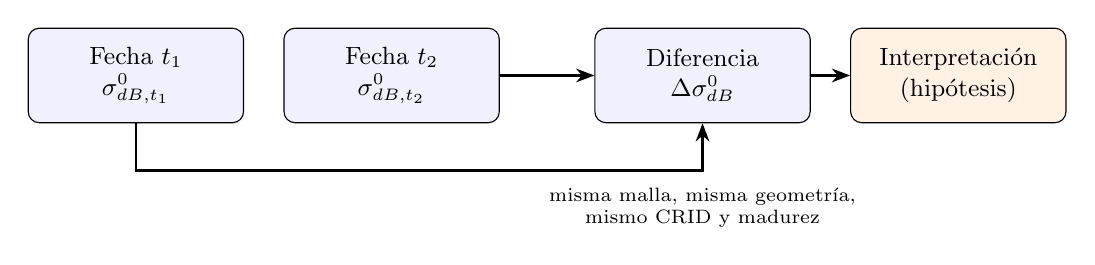
\begin{tikzpicture}[node distance=5mm,
  caja/.style={draw,rounded corners,fill=blue!6,align=center,text width=2.5cm,minimum height=1.2cm,font=\small},
  fl/.style={-{Stealth},thick}]
\node[caja] (a) {Fecha $t_1$\\$\sigma^0_{dB,t_1}$};
\node[caja,right=of a] (b) {Fecha $t_2$\\$\sigma^0_{dB,t_2}$};
\node[caja,right=12mm of b] (c) {Diferencia\\$\Delta\sigma^0_{dB}$};
\node[caja,right=of c,fill=orange!10] (d) {Interpretación (hipótesis)};
\draw[fl] (b)--(c); \draw[fl] (a.south) |- ++(0,-6mm) -| (c.south);
\draw[fl] (c)--(d);
\node[font=\scriptsize,below=7mm of c,text width=5cm,align=center] {misma malla, misma geometría, mismo CRID y madurez};
\end{tikzpicture}
\caption{El cambio se calcula píxel a píxel entre dos escenas comparables y solo después se interpreta. La
interpretación nunca es parte de la medición.}
\label{fig:flujo-delta}
\end{figure}

\subsection{Tres razones por las que dos fechas pueden diferir}

\begin{description}[style=nextline]
  \item[Cambio real de la superficie.] Cambió la humedad del suelo, la presencia de agua, la estructura de
        la vegetación o el uso del suelo. Es lo que se busca.
  \item[Diferencia de adquisición o procesamiento.] Distinta trayectoria, marco, dirección de mirada,
        polarización, versión de procesamiento o madurez del producto. El control de comparabilidad existe
        para eliminar esta fuente.
  \item[Variabilidad estadística.] El moteado de cada fecha es independiente, así que aun sin cambio real el
        $\Delta\sigma^0$ tiene una dispersión.
\end{description}

\subsection{La dispersión que introduce el moteado}

Si en cada fecha el valor en dB tiene desviación estándar $\sigma_L$ por moteado (ecuación~\eqref{eq:db-gamma}),
y las dos fechas son independientes, la desviación de la diferencia es
\begin{equation}
  \sigma_{\Delta} = \sqrt{2}\,\sigma_L .
  \label{eq:sigma-delta}
\end{equation}
Con $L=1$ resulta $\approx7.9$\,dB, con $L=4$ unos $3.3$\,dB y con $L=16$ cerca de $1.6$\,dB
(figura~\ref{fig:delta_distribucion}). Así, un píxel aislado que cambia $+3$\,dB entre dos fechas
\emph{no} permite afirmar nada: está dentro del ruido esperado aun sin cambio.

\figura{delta_distribucion}{0.78}{Distribución de $\Delta\sigma^0_{dB}$ cuando \emph{no} hay cambio real,
solo moteado independiente en cada fecha, para $L=1,4,16$ looks. Simulación de 400\,000 pares.}

La manera de recuperar sensibilidad es agregar. Si se promedian $N$ píxeles independientes de una región
homogénea, la dispersión baja aproximadamente como $1/\sqrt{N}$:
\begin{equation}
  \sigma_{\Delta,\mathrm{región}} \approx \frac{\sqrt2\,\sigma_L}{\sqrt{N_{\mathrm{ind}}}} .
  \label{eq:sigma-region}
\end{equation}
Con $L=4$ y $N_{\mathrm{ind}}=100$ píxeles independientes, la dispersión baja de 3.3 a 0.33\,dB. La palabra
\emph{independientes} es crucial: píxeles vecinos suelen estar correlacionados, y entonces $N_{\mathrm{ind}}$
es menor que el número de píxeles.

\subsection{La anomalía estandarizada}

La anomalía $z$ (planeada, no implementada) responde a una pregunta distinta: no «¿cuánto cambió este píxel?»
sino «¿cuánto cambió respecto a lo que cambia normalmente?». Restar $\mu$ elimina un cambio promedio que afecta
a toda la región (por ejemplo, una diferencia sistemática de calibración o una humedad general), y dividir por
$s$ expresa el resto en unidades de dispersión típica. Un valor $z=3$ indica un píxel que se aleja tres
desviaciones de la referencia. Lo que sea «grande» debe fijarse \emph{antes} de mirar el resultado y registrarse
junto con $\mu$ y $s$; de lo contrario el umbral se ajusta inconscientemente a lo que se quiere ver.

\begin{atencion}
Un $\Delta\sigma^0$ alto no es una detección de inundación, de deforestación ni de ningún otro fenómeno. Es
una diferencia de respuesta radar que, junto con contexto y datos independientes, \emph{puede} apoyar una
hipótesis. La advertencia final de esta sección no es una fórmula de cortesía: es la frontera entre medir e
interpretar.
\end{atencion}

\section{Modelos de dispersión (para interpretar, no para medir)}

\subsection{Tres mecanismos, tres firmas}
\label{sec:modelos}

Los modelos de esta sección sirven para razonar \emph{qué podría estar causando} un cambio medido. Conviene
tener presentes los tres mecanismos básicos con los que la microonda interactúa con la superficie
(figura~\ref{fig:mecanismos}):
\begin{description}[style=nextline]
  \item[Reflexión especular (superficie lisa).] Si la superficie es lisa respecto a la longitud de onda, la
        energía rebota como en un espejo, lejos del satélite, y el píxel se ve oscuro.
  \item[Dispersión difusa o de volumen.] En suelo rugoso o en una copa vegetal, la energía se dispersa en
        muchas direcciones y una parte regresa al radar.
  \item[Doble rebote.] Dos superficies perpendiculares (agua y tronco, suelo y pared) forman un reflector en
        esquina que devuelve una señal intensa en la dirección de incidencia.
\end{description}

\figura{mecanismos}{1.0}{Los tres mecanismos básicos de retrodispersión. En cada panel, la flecha azul es la
señal incidente; la roja, la parte que regresa hacia el radar.}

\begin{table}[htbp]
\centering\small
\begin{tabularx}{\linewidth}{p{.26\linewidth}p{.3\linewidth}X}
\toprule
\textbf{Superficie o escenario} & \textbf{Mecanismo dominante} & \textbf{Respuesta cualitativa esperada}\\\midrule
Agua abierta en calma & Reflexión especular & HH y HV bajos (oscuro).\\
Agua con oleaje o rizado de viento & Rugosidad creciente & Más retorno que en calma; puede confundirse con tierra.\\
Suelo desnudo seco $\to$ húmedo & Mayor constante dieléctrica & Sube el retorno, sobre todo en HH.\\
Bosque denso & Dispersión de volumen & HV relativamente alto; poca sensibilidad al suelo.\\
Vegetación inundada & Doble rebote tronco--agua & Sube HH; efecto opuesto al del agua abierta.\\
Zona urbana & Doble rebote y esquinas & Muy brillante en HH.\\\bottomrule
\end{tabularx}
\caption{Tendencias cualitativas habituales. Las magnitudes dependen del sitio, de la geometría y de la
estación; esta tabla no es un criterio de clasificación.}
\label{tab:escenarios}
\end{table}

\subsection{Rugosidad: criterio de Rayleigh}
\label{sec:rayleigh}
Una superficie se comporta como lisa (reflexión especular, poca señal de vuelta) si la desviación
estándar de su altura $h$ cumple
\begin{equation}
  h < \frac{\lambda}{8\cos\theta_i}.
\end{equation}
El agua en calma cumple este criterio y aparece oscura en la imagen. El suelo rugoso o húmedo
devuelve más señal.

\paragraph{Cómo leer el criterio.} El criterio compara la altura típica de las irregularidades $h$ con una
fracción de la longitud de onda corregida por el ángulo. La razón es de fase: si dos puntos de la superficie
difieren en altura en $h$, los rayos reflejados en ellos difieren en un recorrido $2h\cos\theta_i$. Cuando esa
diferencia es pequeña frente a la longitud de onda (el criterio usa $\lambda/4$, de donde sale el $\lambda/8$),
los rayos se refuerzan en dirección especular y la superficie es «lisa»; cuando no, se dispersan.

\figura{rayleigh}{0.62}{Rugosidad crítica de Rayleigh en banda L en función del ángulo de incidencia. Con
$\lambda=24$\,cm, a $44^\circ$ resulta $4.2$\,cm: por debajo se comporta como lisa; por encima, como rugosa.}

Con $\lambda\approx24$\,cm el umbral es $3.5$\,cm a $30^\circ$, $4.2$\,cm a $44^\circ$ y $6.0$\,cm a
$60^\circ$. Una consecuencia práctica: en banda L, ondas o rizados de unos pocos centímetros sobre un lago ya
pueden dejar de ser «lisos», y el agua se verá más brillante que en calma. La misma superficie puede ser lisa
en banda L y rugosa en banda X, porque el umbral depende de $\lambda$.

\subsection{Dispersión de volumen: \emph{water cloud model}}
Pese a su nombre, no es un modelo de fluidos. Representa el dosel vegetal como una nube de
dispersores (Attema y Ulaby, 1978):
\begin{align}
  \sigma^0 &= A\, V_1 \cos\theta_i \left(1 - T^2\right) + T^2\, \sigma^0_{\text{suelo}}, \\
  T^2 &= \exp\!\left(-\frac{2 B\, V_2}{\cos\theta_i}\right),
\end{align}
donde $V_1$ y $V_2$ son descriptores de la vegetación, $A$ y $B$ son parámetros empíricos que se
ajustan con datos de campo y $T^2$ es la transmisividad de ida y vuelta a través del dosel.

\paragraph{Cómo leer el modelo.} El \emph{water cloud model} es un balance entre dos fuentes de señal. El primer
término, $AV_1\cos\theta_i(1-T^2)$, es lo que dispersa la propia vegetación; crece con la cantidad de vegetación
$V_1$ y se satura porque $(1-T^2)$ no puede pasar de 1. El segundo, $T^2\sigma^0_{suelo}$, es el retorno del
suelo atenuado en su camino de ida y vuelta a través del dosel, y disminuye cuando $V_2$ crece. La
figura~\ref{fig:water_cloud} lo muestra con parámetros \emph{ilustrativos}: para vegetación escasa manda el
suelo; para vegetación densa, el dosel.

\figura{water_cloud}{0.66}{Contribuciones del dosel y del suelo atenuado al $\sigma^0$ total del water cloud
model. Los parámetros $A$, $B$ y $\sigma^0_{suelo}$ son valores de ejemplo escogidos para mostrar la forma de
las curvas; no están calibrados con datos de campo.}

\begin{intuicion}
La consecuencia más importante del modelo es que \emph{la sensibilidad a la humedad del suelo disminuye al
aumentar la vegetación}. Un cambio de humedad se ve bien sobre suelo casi desnudo y se enmascara bajo un dosel
denso. Por eso la misma variación de $\Delta\sigma^0$ no significa lo mismo en dos coberturas distintas.
\end{intuicion}

\subsection{Doble rebote}
El agua bajo vegetación (vegetación inundada) forma un reflector diédrico tronco--agua que
\emph{aumenta} la señal, sobre todo en HH. Es el comportamiento opuesto al del agua abierta, y es
relevante si el fenómeno elegido fuera inundación o humedales.

\section{Interferometría (solo si el caso fuera deformación)}

La diferencia de fase entre dos adquisiciones se relaciona con el desplazamiento en la línea de
vista $\Delta R$:
\begin{equation}
  \Delta\phi = \frac{4\pi}{\lambda}\, \Delta R .
\end{equation}
El signo depende de la convención del producto (GUNW). El resultado es un desplazamiento en línea
de vista, no vertical.

\subsection{Un orden de magnitud para el desplazamiento}

La relación $\Delta\phi=4\pi\Delta R/\lambda$ implica que una vuelta completa de fase ($2\pi$, un \emph{fleco})
corresponde a un desplazamiento en la línea de vista de $\Delta R=\lambda/2$. Con $\lambda\approx24$\,cm, cada
franja equivale a $\approx12$\,cm. La interferometría puede detectar desplazamientos de fracciones de franja,
es decir, de centímetros o menos, pero exige que la fase se mantenga coherente entre las dos fechas. Este
proyecto no usa interferometría: se conserva en el documento solo para delimitar qué pregunta responde y
cuál no.

\section{Ecuaciones de las figuras de la Etapa 1}
\label{sec:figuras}

Las figuras están en
\path{data/explore/NISAR_L2_PR_GCOV_034_062_A_010_4005_DHDH_A_20261028T114006_20261028T114041_P05036_N_F_J_001/figuras/}.
Son de la escena GCOV T62/F10 ASCENDING del 2026-10-28 (P05036), la que se inspeccionó en la Etapa 1 y no tiene pareja. Las genera
\path{python -m pipeline.etapa1} con las funciones de \path{pipeline/etapa1_figuras.py}. Las fórmulas están en
\path{pipeline/nisar_h5.py} y \path{pipeline/etapa1.py}.

\paragraph{Trazabilidad.} Los valores numéricos de esta sección se copiaron de \path{metadatos.json} de esa misma carpeta (creado el
2026-11-13, \texttt{version\_codigo = 98f7e07-dirty}). El sufijo \texttt{-dirty} indica que había cambios sin commit cuando se generó;
para citar estas cifras conviene regenerar la carpeta con el árbol de git limpio.

\paragraph{Regla.} Las figuras son para \emph{ver}. Ningún número se calcula sobre los PNG (\texttt{AGENTS.md} §5): todo sale del
\texttt{.h5} y queda en \path{metadatos.json} y \path{control/*.csv}.

\subsection{Pasos comunes a todas las figuras}

\paragraph{Potencia del producto.} En GCOV las capas \texttt{HHHH} y \texttt{HVHV} ya son potencia lineal en la convención que declara
el archivo (\path{rtc/outputBackscatterNormalizationConvention = gamma0}). El programa no la transforma:
\begin{equation}
  \gamma^0_{pq}(x,y) = \texttt{capa}_{pqpq}(x,y), \qquad pq \in \{\text{HH}, \text{HV}\}.
\end{equation}

\paragraph{De \gz{} a \sz.} Con la capa \path{rtcGammaToSigmaFactor} ($F$) que trae el producto, píxel a píxel:
\begin{equation}
  \sigma^0(x,y) = \gamma^0(x,y)\, F(x,y).
  \label{eq:gamma-sigma}
\end{equation}
En terreno plano, por la sección~\ref{sec:retro}, se esperaría $F \approx \cos\theta_i$. El producto calcula $F$ con el modelo de elevación, por lo
que en relieve no es exactamente $\cos\theta_i$.

\paragraph{Píxeles válidos.} Un píxel entra al análisis si su máscara no es 0 (no válido) ni 255 (fuera de la adquisición) y si cae
dentro del polígono de la ROI:
\begin{equation}
  \text{válido}(x,y) \iff \texttt{mask}(x,y) \notin \{0, 255\} \;\wedge\; (x,y) \in \text{ROI}.
\end{equation}
Los demás se ponen en NaN.

\paragraph{Decibeles.} Se usa la ecuación~\eqref{eq:db}. Si $X \le 0$ o es NaN, el resultado es NaN (no se toma el logaritmo de
cero).

\paragraph{Multilook $n\times n$.} Se promedia en \emph{lineal} y después se pasa a dB. Para el bloque $B$ de $n\times n$ píxeles, con
$N_v$ píxeles válidos:
\begin{equation}
  \bar{P}_B = \frac{1}{N_v}\sum_{k \in B,\ \text{válido}} P_k,
  \qquad
  \bar{P}_{B,\text{dB}} = 10\log_{10}\bar{P}_B,
  \qquad
  \bar{P}_B = \text{NaN si } N_v < 0.5\,n^2 .
  \label{eq:multilook}
\end{equation}
\textbf{En qué se basa:} el moteado (\emph{speckle}) del radar es multiplicativo. Promediar potencias reduce su varianza sin sesgo,
mientras que promediar dB da un valor sistemáticamente menor (ver la figura C). En la Etapa 1, $n = 2$ para GCOV.

\subsection{\texttt{A\_vista\_general\_HHHH.png}: vista general de la escena}

\textbf{Qué muestra:} \gz{} HH en \emph{lineal} sobre toda la escena (33\,480\,\por\,34\,128 píxeles de 10\,m), con el contorno de la
ROI en rojo. Azul = sin dato. Función: \path{overview()}.

\textbf{Submuestreo.} Se toma 1 de cada $s = 50$ píxeles en filas y columnas, sin promediar (cada punto de la vista representa 500\,m):
\begin{equation}
  v_{ij} = \gamma^0_{\text{HH}}(s\,i,\ s\,j).
\end{equation}
Por eso la vista conserva el moteado: es una muestra, no un promedio.

\textbf{Normalización del color (\texttt{PowerNorm}).} Con los percentiles 5 y 95 de la vista, $p_b$ y $p_a$, y $\gamma_v = 0.5$:
\begin{equation}
  t = \left[\operatorname{clip}\!\left(\frac{v - p_b}{p_a - p_b},\, 0,\, 1\right)\right]^{\gamma_v},
\end{equation}
donde $t\in[0,1]$ es el tono de gris (0 negro, 1 blanco). Las marcas de la barra de color están equiespaciadas en $t$, por eso valen
\begin{equation}
  v(t) = p_b + (p_a - p_b)\, t^{1/\gamma_v}, \qquad t = 0,\ 0.2,\ \ldots,\ 1 .
\end{equation}

\textbf{Valores de esta figura:} $p_b = 0.0306$, $p_a = 0.5458$; marcas 0.031, 0.051, 0.113, 0.216, 0.360, 0.546. Comprobación:
$v(0.2) = 0.0306 + 0.5152\cdot 0.2^{2} = 0.0512$.

\textbf{En qué se basa:} $\gamma_v < 1$ aclara los valores bajos para que se distingan las zonas oscuras. Es solo visualización: este
$\gamma_v$ no es la $\gamma$ de \gz.

\paragraph{Cómo leer la normalización del color.} La función de la figura es repartir los valores en una escala
de grises con más detalle en los tonos oscuros. Con $\gamma_v=0.5$, la curva que lleva el valor $v$ al tono
$t$ es una raíz cuadrada, que «abre» los valores bajos. La figura~\ref{fig:powernorm} la compara con la
correspondencia lineal y marca los seis valores de la barra de color (0.031, 0.051, 0.113, 0.216, 0.360 y
0.546), que están equiespaciados en tono pero no en valor.

\figura{powernorm}{0.62}{Correspondencia entre el valor $\gamma^0_{HH}$ (lineal) y el tono de gris en la figura
A. Las marcas de la barra de color son equiespaciadas en $t$, no en $v$.}

\figura{escalas_pixel}{1.0}{Cambios de escala entre las figuras de la Etapa 1. El producto tiene píxeles de
10\,m; las figuras B y B2 usan promedios $2\times2$ (20\,m); la figura A toma una muestra de 1 cada 50 píxeles
sin promediar (cada punto representa 500\,m).}

\subsection{\texttt{B\_roi\_gamma0\_dB.png}: ROI en dB (\gz)}

\textbf{Qué muestra:} \gz{} HH y HV dentro de la ventana de la ROI, en dB tras multilook $2\times2$ (píxel de 20\,m). Función:
\path{roi_db()}.

\textbf{Ecuaciones:} multilook~\eqref{eq:multilook} con $n = 2$ y después dB~\eqref{eq:db}.

\textbf{Escala común.} Ambas polarizaciones usan el mismo rango de color, los percentiles 2 y 98 de los valores en dB de \emph{las dos}
juntas, para que sus tonos sean comparables. En esta figura: $-19.36$ a $-3.10$\,dB.

\textbf{Lectura:} HV se ve más oscura que HH porque la retrodispersión con polarización cruzada suele ser menor. En la ROI, la media de
los dB es $-8.06$\,dB en HH y $-13.50$\,dB en HV (tabla de la figura C).

\paragraph{El multilook paso a paso.} La figura~\ref{fig:multilook_bloques} muestra cómo se agrupan los
píxeles de $2\times2$ y qué ocurre cuando faltan datos. La regla de la ecuación~\eqref{eq:multilook} exige al
menos $0.5\,n^2=2$ píxeles válidos por bloque; si no, el bloque queda en NaN.

\figura{multilook_bloques}{0.52}{Ejemplo con valores ilustrativos de potencia lineal en un arreglo de
$4\times4$ píxeles. Los cuatro bloques de $2\times2$ tienen 4, 2, 4 y 1 píxeles válidos.}

\begin{table}[htbp]
\centering\small
\begin{tabular}{cccc}
\toprule
Bloque & Píxeles válidos $N_v$ & Media lineal & Resultado en dB\\\midrule
superior izquierdo & 4 & 0.125 & $-9.03$\\
superior derecho & 2 & 0.275 & $-5.61$\\
inferior izquierdo & 4 & 0.130 & $-8.86$\\
inferior derecho & 1 & (descartado) & NaN\\\bottomrule
\end{tabular}
\caption{Resultado del multilook del ejemplo de la figura~\ref{fig:multilook_bloques}. El bloque inferior
derecho tiene $N_v=1<2$ y se marca como NaN.}
\label{tab:bloques}
\end{table}

\paragraph{Por qué una escala común.} Al usar los mismos percentiles 2 y 98 de HH y HV juntos, los tonos de
ambas figuras se pueden comparar directamente: si HV se ve más oscura es porque su valor es menor, no porque
se estiró distinto.

\subsection{\texttt{B2\_roi\_sigma0\_dB.png}: ROI en dB (\sz)}

\textbf{Qué muestra:} lo mismo que la figura B, pero con \sz{} calculada con~\eqref{eq:gamma-sigma} antes del multilook. Escala común:
$-20.91$ a $-4.54$\,dB.

\textbf{Relación con B:} en dB, la conversión es una suma,
\begin{equation}
  \sigma^0_{\text{dB}} = \gamma^0_{\text{dB}} + 10\log_{10} F .
\end{equation}
\textbf{Comprobación de orden de magnitud:} en la ROI la media de los dB de HH pasa de $-8.06$ (\gz) a $-9.79$ (\sz), una diferencia de
$-1.73$\,dB. Con el ángulo de incidencia medio de la ROI (figura E, $43.9^\circ$), terreno plano daría
$10\log_{10}\cos 43.9^\circ \approx -1.43$\,dB. Son del mismo orden; la diferencia es esperable porque $F$ incluye el relieve.

\subsection{\texttt{C\_histogramas\_gamma0\_dB.png}: histogramas de \gz{} en dB}

\textbf{Qué muestra:} la distribución de \gz{} en dB en la \emph{resolución completa} del producto (sin multilook), para todos los
píxeles válidos de la ROI ($n = 14\,699\,442$ por polarización). Función: \path{histograms()}; estadísticas: \path{power_stats()}.

\textbf{Histograma.} Clases de 0.1\,dB entre $-60$ y $30$\,dB. El eje vertical es el porcentaje de píxeles en cada clase:
\begin{equation}
  h_k = 100\,\frac{\#\{\,i : \gamma^0_{\text{dB},i} \in [a_k, a_k + 0.1)\,\}}{n}\ \mathrm{\%}.
\end{equation}
El eje horizontal se recorta a los percentiles 0.2 y 99.8 de la distribución acumulada, solo para verla mejor.

\textbf{Líneas y franja.} Con $P_i$ la potencia lineal y $D_i = 10\log_{10}P_i$:
\begin{align}
  \text{media de los dB} &= \frac{1}{n}\sum_i D_i, \\
  \text{dB de la media lineal} &= 10\log_{10}\!\left(\frac{1}{n}\sum_i P_i\right), \\
  \text{mediana} &= \operatorname{mediana}(D_i), \qquad \text{franja azul} = [\,p_5(D),\ p_{95}(D)\,].
\end{align}

\textbf{En qué se basa: desigualdad de Jensen.} Como el logaritmo es cóncavo,
\begin{equation}
  \frac{1}{n}\sum_i 10\log_{10}P_i \;\le\; 10\log_{10}\!\left(\frac{1}{n}\sum_i P_i\right).
\end{equation}
Por eso la línea punteada (dB de la media) siempre queda a la derecha de la continua (media de los dB). Como referencia teórica, si
$P$ siguiera una distribución exponencial (moteado completamente desarrollado, un solo look, superficie homogénea), la diferencia
sería exactamente $10\log_{10}(e)\cdot\gamma_E \approx 2.51$\,dB, con $\gamma_E \approx 0.5772$ la constante de Euler--Mascheroni.
Con varios looks esa diferencia es menor.

\textbf{Valores de esta figura:}

\begin{longtable}{lrr}
\toprule
 & \textbf{HH} & \textbf{HV} \\
\midrule
Media de los dB & $-8.055$ & $-13.503$ \\
Mediana (dB) & $-7.880$ & $-13.173$ \\
dB de la media lineal & $-3.786$ & $-9.226$ \\
Diferencia (dB de la media $-$ media de los dB) & $4.27$ & $4.28$ \\
$p_5$ a $p_{95}$ (dB) & $-14.07$ a $-2.85$ & $-20.00$ a $-8.11$ \\
Desviación estándar (dB) & $3.59$ & $3.73$ \\
\bottomrule
\end{longtable}

\textbf{Lectura (inferencia, no medición):} la diferencia observada ($\approx 4.3$\,dB) es mayor que la del moteado puro (2.51\,dB).
Lo esperable es que se deba a que la ROI mezcla coberturas distintas y tiene algunos píxeles muy brillantes que elevan la media lineal
(el máximo de HH en la escena completa es 7418, según los atributos del \texttt{.h5}). No se ha verificado cuál de los dos efectos
domina.

\paragraph{Un experimento mental con histogramas gaussianos en dB.} Para dimensionar la brecha de 4.27\,dB entre
el dB de la media lineal y la media de los dB, conviene compararla con tres referencias.
\begin{enumerate}
  \item Si los valores en dB fueran \emph{gaussianos} con media $\mu$ y desviación $s$, la brecha sería
        \begin{equation}
          \Delta_J = \frac{\ln 10}{20}\,s^2 \approx 0.1151\,s^2 ,
          \label{eq:jensen-gauss}
        \end{equation}
        que con $s=3.59$\,dB da $1.48$\,dB.
  \item Si el moteado de un solo look fuera lo único, la brecha sería $2.51$\,dB.
  \item La brecha observada es $4.27$\,dB en HH y $4.28$\,dB en HV, mayor que ambas.
\end{enumerate}

\figura{jensen_gauss}{0.64}{Referencia gaussiana. Se dibuja un histograma gaussiano en dB con la media y la
desviación observadas en HH ($-8.055$ y $3.59$\,dB). Para ese caso, el dB de la media lineal caería en
$-6.57$\,dB, mucho más a la izquierda que el valor observado, $-3.786$\,dB.}

Los dos números dicen algo sobre la \emph{forma} del histograma: el observado tiene una cola brillante más
pesada que la gaussiana, lo que eleva la media lineal. Esto concuerda con la lectura de la sección
(\emph{inferencia, no medición}): una región que mezcla coberturas y tiene píxeles muy brillantes.

\begin{ejemplo}[Una cota para el número efectivo de looks]
La desviación estándar de HH en la ROI es $3.59$\,dB. El moteado de un solo look produciría por sí solo
$5.57$\,dB, \emph{más} que lo observado, así que el producto no puede ser de un look efectivo. Resolviendo
$4.34\sqrt{\psi'(L)}=3.59$ se obtiene $L\approx1.9$. Como la textura real de la escena también aporta
varianza, el número efectivo de looks es al menos del orden de 2. Es una inferencia razonable, pero no una
medición: depende de suponer que el histograma está dominado por moteado más textura.
\end{ejemplo}

\subsection{\texttt{D\_mascara.png}: máscara del producto}

\textbf{Qué muestra:} las categorías de la capa \texttt{mask} en la ventana rectangular de la ROI. Función: \path{mask_map()}.

\begin{longtable}{p{0.40\linewidth}p{0.20\linewidth}p{0.28\linewidth}}
\toprule
\textbf{Categoría} & \textbf{Regla} & \textbf{\% de la ventana} \\
\midrule
No válido (rojo) & $\texttt{mask} = 0$ & 0.391 \\
Válido, subfranja (verde) & $\texttt{mask} \notin \{0,255\}$ & 99.393 \\
Fuera de la adquisición (azul) & $\texttt{mask} = 255$ & 0.000 \\
Fuera del polígono ROI (gris) & fuera del polígono & 0.217 \\
\bottomrule
\end{longtable}

\textbf{Porcentajes.} Se calculan con \emph{todos} los píxeles de la ventana ($N = 2687 \times 5504$), aunque la imagen muestre solo 1
de cada $s$ píxeles, con $s = \lceil \max(\text{forma}) / 2000 \rceil = \lceil 5504/2000 \rceil = 3$:
\begin{equation}
  P_c = 100\,\frac{N_c}{N}\,\mathrm{\%}.
\end{equation}

\textbf{Relación con la cobertura de la ROI.} La cobertura que se reporta en otros documentos (99.61\,\%) se mide sobre el
\emph{polígono}, no sobre el rectángulo:
\begin{equation}
  \text{cobertura} = 100\,\frac{N_{\text{válido}}}{N_{\text{polígono}}}
  = \frac{99.393}{100 - 0.217}\times 100 \approx 99.61\,\mathrm{\%}.
\end{equation}

\textbf{Precaución:} la máscara indica \emph{dónde} no hay dato válido, no \emph{por qué}. En esta escena el producto no aplica
máscara de sombra/layover (\path{shadowMaskingApplied = False}), así que esas zonas no están necesariamente en rojo.

\paragraph{Comprobación de las cifras.} La ventana rectangular de la ROI tiene $2687\times5504=14\,789\,248$
píxeles. Los $14\,699\,442$ píxeles válidos dentro del polígono representan $14\,699\,442/14\,789\,248=99.393\,\mathrm{\%}$
de la ventana, que coincide con la fila «Válido» de la tabla. La cobertura de $99.61\,\mathrm{\%}$ se divide entre los
píxeles del \emph{polígono}, que son los de la ventana menos los $0.217\,\mathrm{\%}$ que caen fuera de él.

\figura{ventana_roi}{0.55}{Esquema de la ventana rectangular y del polígono de la ROI. Dentro del polígono
hay píxeles válidos y una franja angosta con \texttt{mask}~$=0$; fuera, píxeles que no se analizan.}

\subsection{\texttt{E\_incidencia.png}: ángulo de incidencia}

\textbf{Qué muestra:} el ángulo de incidencia $\theta_i$ sobre la ROI, leído del cubo \path{metadata/radarGrid/incidenceAngle} del
producto (malla de 500\,m). Es la capa de 500\,m de altura sobre el elipsoide. Función: \path{incidence()}; lectura:
\path{read_incidence()} en \path{nisar_h5.py}. El programa \emph{no calcula} el ángulo: lo lee del producto.

\paragraph{Verificación.} Todo lo de esta subsección se comprobó con el \texttt{.h5} local de la escena
(\path{H5 FILES/NISAR_L2_PR_GCOV_034_..._P05036_N_F_J_001.h5}) el 2026-11-14. Las descripciones entre comillas son los atributos
\texttt{description} de cada capa. Los números son medias sobre los nodos del cubo dentro del rectángulo de la ROI. La figura añade un
nodo de margen por lado, por eso su barra de color llega a $42.34^\circ$--$45.41^\circ$.

\subsubsection*{1. El elipsoide de referencia (WGS84)}

La Tierra se aproxima con un elipsoide de revolución, el WGS84:
\begin{equation}
  a = 6\,378\,137\ \text{m}, \qquad f = \frac{1}{298.257223563}, \qquad b = a(1-f) \approx 6\,356\,752\ \text{m},
\end{equation}
donde $a$ es el radio ecuatorial, $b$ el polar y $f$ el achatamiento. El producto declara sus alturas sobre este elipsoide:
\path{heightAboveEllipsoid} = «Height values above WGS84 Ellipsoid».

\begin{itemize}
  \item \textbf{Altura elipsoidal $h$:} distancia sobre el elipsoide, medida a lo largo de su normal. Es la que usa el cubo.
  \item \textbf{Altura ortométrica $H$} (la «altura sobre el nivel del mar» de los mapas y de muchos DEM): se mide sobre el geoide. Se
        relacionan con la ondulación del geoide $N$, que depende del lugar:
        \begin{equation}
          h = H + N .
        \end{equation}
        Para usar la elevación de un DEM con este cubo hay que convertirla a altura elipsoidal.
  \item \textbf{Normal al elipsoide $\hat{\mathbf n}$:} la dirección «hacia arriba» en cada punto. No pasa exactamente por el centro de
        la Tierra (latitud geodésica $\neq$ geocéntrica). En la latitud de la ROI ($\approx 16.8^\circ$) la diferencia es de
        $\approx 0.1^\circ$.
  \item \textbf{Radio geocéntrico} del elipsoide a la latitud geodésica $\varphi$:
        \begin{equation}
          R(\varphi) = \sqrt{\frac{(a^2\cos\varphi)^2 + (b^2\sin\varphi)^2}{(a\cos\varphi)^2 + (b\sin\varphi)^2}}
          \;\approx\; 6376.4\ \text{km} \quad (\varphi = 16.8^\circ).
        \end{equation}
\end{itemize}

\subsubsection*{2. Definición del ángulo de incidencia}

Según el producto, \path{incidenceAngle} es «the angle between the LOS vector and the normal to the ellipsoid at the target height».
Con $\hat{\mathbf l}$ el vector unitario de la línea de vista (\emph{line of sight}, LOS), del blanco al sensor:
\begin{equation}
  \cos\theta_i = \hat{\mathbf l}\cdot\hat{\mathbf n}.
  \label{eq:incidencia}
\end{equation}
El producto da $\hat{\mathbf l}$ en coordenadas locales este--norte--arriba (ENU), pero solo sus componentes horizontales
(\path{losUnitVectorX} = este, \path{losUnitVectorY} = norte). Como el vector es unitario, la componente vertical (la normal) se obtiene así:
\begin{equation}
  l_U = \sqrt{1 - l_E^2 - l_N^2}, \qquad \theta_i = \arccos l_U .
\end{equation}
\textbf{Comprobación:} en la ROI, $\arccos l_U$ y \path{incidenceAngle} difieren como máximo en $1.1\times10^{-5}$ grados.

En la ROI, $\overline{l_E} = 0.676$ y $\overline{l_N} = 0.153$: el sensor está al este (y algo al norte) de los blancos. Concuerda con
el producto: órbita ascendente (\path{orbitPassDirection = Ascending}), que vuela hacia el norte, y radar que mira a la izquierda
(\path{lookDirection = Left}), es decir, hacia el oeste.

\textbf{Ángulo de incidencia elipsoidal frente a local.} $\theta_i$ usa la normal del \emph{elipsoide}, no la pendiente del terreno. El
ángulo de incidencia \emph{local} usa la normal del terreno $\hat{\mathbf n}_t$, calculada con un DEM:
\begin{equation}
  \cos\theta_{\text{loc}} = \hat{\mathbf l}\cdot\hat{\mathbf n}_t .
\end{equation}
En una ladera que mira al radar, $\theta_{\text{loc}} < \theta_i$ (más señal, posible \emph{layover}); en una que le da la espalda,
$\theta_{\text{loc}} > \theta_i$ (menos señal, posible sombra si $\theta_{\text{loc}} \ge 90^\circ$). La figura E \textbf{no} muestra
$\theta_{\text{loc}}$.

\subsubsection*{3. Geometría satélite--Tierra: por qué $\theta_i$ vale unos $44^\circ$}
Se considera el triángulo formado por el centro de la Tierra $O$, el satélite $S$ y el blanco $T$:
\begin{itemize}
  \item $R_s = |OS|$: radio de la órbita. Media de \path{metadata/orbit/position}: $R_s = 7128.6$\,km (unos 750\,km de altura).
  \item $R_t = |OT| = R(\varphi) + h$: radio del blanco.
  \item $r = |ST|$: distancia en línea de vista (\path{slantRange}). En la ROI va de 976.8 a 1018.1\,km (media 997.2\,km).
  \item $\theta_e$: ángulo de elevación en el satélite, entre la LOS y la vertical del sensor (\path{elevationAngle}). Media:
        $38.31^\circ$.
  \item $\theta_i$: ángulo de incidencia en el blanco. Media: $43.87^\circ$ (capa de 0\,m).
  \item $\alpha$: ángulo en el centro de la Tierra entre satélite y blanco.
\end{itemize}

\textbf{Ley de los senos.} En el triángulo $OST$, el ángulo en $S$ es $\theta_e$ y el ángulo en $T$ es $180^\circ - \theta_i$:
\begin{equation}
  \frac{R_t}{\sin\theta_e} = \frac{R_s}{\sin\theta_i}
  \quad\Longrightarrow\quad
  \sin\theta_i = \frac{R_s}{R_t}\,\sin\theta_e .
  \label{eq:senos}
\end{equation}
Como $R_s > R_t$, siempre $\theta_i > \theta_e$: la curvatura de la Tierra hace que el blanco «vea» al radar más inclinado de lo que
el radar lo mira a él.

\textbf{Suma de ángulos.} En el mismo triángulo, $\theta_e + (180^\circ - \theta_i) + \alpha = 180^\circ$:
\begin{equation}
  \theta_i = \theta_e + \alpha .
\end{equation}
En la ROI, $\theta_i - \theta_e = 5.56^\circ$, que corresponde a una distancia sobre el suelo de $R\,\alpha \approx 619$\,km desde el
punto bajo el satélite (nadir).

\textbf{Ley de los cosenos} (relaciona la distancia con el ángulo):
\begin{equation}
  R_s^2 = R_t^2 + r^2 + 2\,R_t\, r\cos\theta_i .
  \label{eq:cosenos}
\end{equation}

\textbf{Comprobación con el producto:} despejando $R_t$ de~\eqref{eq:senos} con los valores de la ROI sale $6376.4$\,km, y
de~\eqref{eq:cosenos}, $6376.1$\,km. El radio geocéntrico WGS84 a $16.8^\circ$ es $6376.4$\,km. La diferencia (menos de 0.3\,km) se
debe a que la normal al elipsoide no apunta exactamente al centro de la Tierra.

\subsubsection*{4. ¿Por qué el cubo tiene capas de altura?}

El producto está en una malla de mapa (EPSG:32615): cada nodo es una posición $(x, y)$ fija. Pero la geometría depende de a qué
altura esté el terreno en ese punto. Por eso \path{radarGrid} es un cubo de $21 \times 682 \times 695$ (altura \por{} $y$ \por{} $x$)
con 21 capas, de $-1000$ a $9000$\,m cada 500\,m. Así, quien conozca la altura real del terreno puede interpolar la geometría
correcta.

\textbf{Variación con la altura.} Si el blanco sube $\Delta h$ en la misma posición $(x,y)$, queda más cerca del satélite y la LOS se
inclina más. Aproximación de Tierra plana, con $D$ la distancia horizontal al nadir y $H_s$ la altura del satélite:
\begin{equation}
  \tan\theta_i = \frac{D}{H_s - h}
  \quad\Longrightarrow\quad
  \frac{\partial\theta_i}{\partial h} = \frac{D}{(H_s-h)^2 + D^2} = \frac{\sin\theta_i}{r}\quad[\text{rad/m}].
\end{equation}
Con $\theta_i = 43.87^\circ$ y $r = 997.2$\,km, de 0 a 500\,m se esperan
$\frac{\sin 43.87^\circ}{997\,238\ \text{m}}\cdot 500\ \text{m} = 0.01991^\circ$. En el producto, la media sube de $43.874^\circ$ a
$43.894^\circ$: $0.01990^\circ$. Coinciden.

\textbf{Elección de la capa en la Etapa 1.} Se toma la capa más cercana a la altura pedida ($h_0 = 500$\,m, opción
\path{--altura-incidencia}), sin interpolar:
\begin{equation}
  k^\ast = \arg\min_k \lvert h_k - h_0 \rvert .
\end{equation}
La altura de 500\,m es un parámetro fijo, no la altura real del terreno de la ROI (que no se ha consultado). Si el terreno estuviera,
por ejemplo, 1000\,m más arriba o más abajo, el error sería de solo $\approx 0.04^\circ$: para una figura de inspección es despreciable.
Para un cálculo píxel a píxel habría que usar la altura elipsoidal del DEM, $h_t$, e interpolar entre las dos capas vecinas:
\begin{equation}
  \theta_i(h_t) \approx \theta_{i,k} + \frac{h_t - h_k}{h_{k+1} - h_k}\,\bigl(\theta_{i,k+1} - \theta_{i,k}\bigr),
  \qquad h_k \le h_t < h_{k+1}.
\end{equation}
Esto \textbf{no} está implementado.

\subsubsection*{5. Por qué el ángulo cambia de este a oeste}

Al alejarse del sensor sobre el suelo una distancia $\Delta g$ (en la dirección horizontal de la LOS), $\theta_i$ crece por dos
motivos: la LOS se inclina más (término de Tierra plana) y la normal local gira por la curvatura (término $1/R$):
\begin{equation}
  \frac{\partial\theta_i}{\partial g} \approx \frac{\cos\theta_i}{r} + \frac{1}{R_t}\quad[\text{rad/m}].
\end{equation}
Con los valores de la ROI esto da $0.0504^\circ$/km. El eje $x$ (este) no es exactamente la dirección de la LOS: la componente
horizontal de la LOS apunta a $\arctan(0.153/0.676) \approx 13^\circ$ al norte del este, así que hay que multiplicar por
$\cos 13^\circ = 0.975$: se esperan $0.049^\circ$/km. Ajustando una recta a $\theta_i$ contra $x$ en la ROI se obtienen
$-0.0489^\circ$/km. El signo es negativo porque ir al este es acercarse al sensor. En los 55\,km de ancho de la ROI son unos
$2.7^\circ$. La componente norte de la LOS añade unos $0.3^\circ$ más a lo largo de los \textasciitilde 27\,km de alto
($0.0504 \cdot \sin 13^\circ \approx 0.011^\circ$/km). Eso explica el rango total en la ROI: $42.35^\circ$ (esquina noreste) a
$45.36^\circ$ (esquina suroeste), unos $3.0^\circ$.

\subsubsection*{6. Para qué sirve $\theta_i$ en este proyecto}

\begin{itemize}
  \item \textbf{Normalización:} en terreno plano, $\gamma^0 = \sigma^0/\cos\theta_i$ (sección~\ref{sec:retro}). Con $\theta_i$ entre $42.3^\circ$ y
        $45.4^\circ$, $10\log_{10}\cos\theta_i$ va de $-1.31$ a $-1.53$\,dB: una variación de unos 0.2\,dB de un lado a otro de la ROI.
  \item \textbf{Rugosidad:} criterio de Rayleigh (sección~\ref{sec:rayleigh}). Con $\lambda \approx 24$\,cm y $\theta_i \approx 44^\circ$, una
        superficie se comporta como lisa si su rugosidad $\delta h < 0.24/(8\cos 44^\circ) \approx 4$\,cm.
  \item \textbf{Comparabilidad:} dos fechas de la misma trayectoria y marco tienen casi la misma geometría, y por eso el mismo
        $\theta_i$ en cada píxel. Es una de las razones por las que solo se comparan escenas con la misma trayectoria, marco y
        dirección.
\end{itemize}

\label{sec:incidencia}
\paragraph{Una imagen de la geometría.} La figura~\ref{fig:triangulo_ost} dibuja el triángulo $OST$ de la
subsección 3, con los lados $R_s$, $R_t$ y $r$ y los ángulos $\theta_e$, $\theta_i$ y $\alpha$. La Tierra
curva hace que $\theta_i>\theta_e$ por el ángulo $\alpha$ subtendido en el centro: con los datos de la ROI,
$\alpha=43.87^\circ-38.31^\circ=5.56^\circ$, que equivale a un arco de $\approx619$\,km sobre el suelo.

\figura{triangulo_ost}{0.5}{Triángulo formado por el centro de la Tierra $O$, el satélite $S$ y el blanco $T$.
Esquema: los ángulos y los lados no están a escala.}

\paragraph{Comprobación numérica con los datos de la ROI.} Con $R_s=7128.6$\,km, $\theta_e=38.31^\circ$ y
$\theta_i=43.87^\circ$, la ley de los senos da $R_t=R_s\sin\theta_e/\sin\theta_i=6376.6$\,km; la ley de los
cosenos con $r=997.2$\,km da $6376.1$\,km. Ambos concuerdan con el radio geocéntrico WGS84 a $16.8^\circ$ de
latitud ($6376.4$\,km) en menos de $0.3$\,km.

\figura{incidencia_roi}{1.0}{Izquierda: el ángulo de incidencia cambia unos $3^\circ$ a lo largo de la ROI,
de $\approx45.4^\circ$ en el oeste a $\approx42.3^\circ$ en el este (esquema lineal con la pendiente
$-0.049^\circ$/km). Derecha: la corrección de terreno plano $10\log_{10}\cos\theta_i$ varía solo
$\approx0.2$\,dB en ese intervalo ($-1.31$ a $-1.54$\,dB).}


\subsection{Resumen: qué ecuación usa cada figura}

\begin{longtable}{p{0.30\linewidth}p{0.62\linewidth}}
\toprule
\textbf{Figura} & \textbf{Ecuaciones} \\
\midrule
\endhead
\texttt{A\_vista\_general\_HHHH} & Submuestreo 1 de cada 50; \texttt{PowerNorm} con percentiles 5--95 y $\gamma_v = 0.5$ (solo color). Sin dB. \\
\texttt{B\_roi\_gamma0\_dB} & Multilook $2\times2$ en lineal~\eqref{eq:multilook} \flecha{} dB~\eqref{eq:db}; escala común percentiles 2--98. \\
\texttt{B2\_roi\_sigma0\_dB} & $\sigma^0 = \gamma^0 F$~\eqref{eq:gamma-sigma} \flecha{} multilook \flecha{} dB. \\
\texttt{C\_histogramas\_gamma0\_dB} & dB por píxel; histograma de 0.1\,dB; media, mediana, dB de la media, $p_5$--$p_{95}$; desigualdad de Jensen. \\
\texttt{D\_mascara} & Clasificación por valor de \texttt{mask}; porcentajes sobre la ventana y cobertura sobre el polígono. \\
\texttt{E\_incidencia} & Lectura de $\theta_i$ del producto en la capa de altura más cercana a 500\,m. Geometría: $\cos\theta_i = \hat{\mathbf l}\cdot\hat{\mathbf n}$, ley de los senos~\eqref{eq:senos}, $\partial\theta_i/\partial h = \sin\theta_i/r$. \\
\bottomrule
\end{longtable}

Ninguna figura usa ecuaciones de fluidos.

\section{Ecuaciones de fluidos y su relación con el radar}

El radar no usa ecuaciones de fluidos. Estas aparecen solo fuera de la cadena radar: la
Parte~\ref{part:inundacion} documenta un simulador hidráulico exploratorio (LISFLOOD-FP, aguas someras)
alimentado con lluvia \emph{sintética} sobre el relieve de NASADEM. Ese simulador es independiente de las
escenas de NISAR: no se usa para medir ni para explicar un $\Delta\sigma^0$, y no se atribuye al radar
ninguna profundidad ni causa de cambio. La metodología del proyecto pide validar con datos independientes
(precipitación, Sentinel-2/HLS, OPERA), no con modelos.

\section*{Referencias de la Parte~\ref{part:radar}}
\addcontentsline{toc}{section}{Referencias de la Parte~\ref{part:radar}}
\begin{itemize}
  \item Documentación NISAR (ASF): \url{https://nisar-docs.asf.alaska.edu/}
  \item Ulaby, F.~T. y Long, D.~G. (2014). \emph{Microwave Radar and Radiometric Remote Sensing}.
        University of Michigan Press.
  \item Attema, E.~P.~W. y Ulaby, F.~T. (1978). Vegetation modeled as a water cloud.
        \emph{Radio Science}, 13(2), 357--364.
  \item Small, D. (2011). Flattening gamma: radiometric terrain correction for SAR imagery.
        \emph{IEEE Transactions on Geoscience and Remote Sensing}, 49(8), 3081--3093.
\end{itemize}

\clearpage

\clearpage
\part{Del píxel al análisis}
\label{part:pixel}

Las partes anteriores explican cada ecuación por separado. Esta parte las sigue \emph{en el orden en que se
aplican}: toma un píxel del archivo \texttt{.h5} y lo acompaña hasta que se convierte en una cifra de una
tabla, en un tono de una figura o en una diferencia entre dos fechas. Los números de los ejemplos son
ilustrativos salvo que se indique lo contrario; las cifras de la escena de la Etapa 1 se citan con su
procedencia.

\section{Qué es un píxel de un GCOV}
\label{sec:que-es-pixel}

Un píxel de \texttt{HHHH} es un número real positivo: la potencia retrodispersada por una celda de unos
10\,m$\times$10\,m del suelo, promediada con vecinas durante la generación del producto, y expresada como
coeficiente $\gamma^0$ lineal. Conviene fijar tres ideas.
\begin{enumerate}
  \item \textbf{No es una medición puntual.} Es un promedio espacial, con su propio moteado residual. La
        figura~\ref{fig:speckle_imagen} mostró cuánta variabilidad hay aun sobre una superficie uniforme.
  \item \textbf{Es adimensional.} $\gamma^0$ es una razón entre potencia devuelta y una referencia de
        área. Las unidades no son vatios ni metros.
  \item \textbf{Su valor típico es menor que 1.} En escala lineal, la mayoría de las superficies naturales
        devuelven una fracción pequeña, y por eso el máximo de HH de la escena completa (7418, según los
        atributos del \texttt{.h5}) corresponde a objetos excepcionales y muy brillantes.
\end{enumerate}

\section{El recorrido de un píxel, paso a paso}
\label{sec:recorrido}

La figura~\ref{fig:recorrido} resume los pasos que sigue cada píxel en la Etapa 1. Las secciones siguientes
detallan cada uno con un número concreto.

\begin{figure}[htbp]
\centering
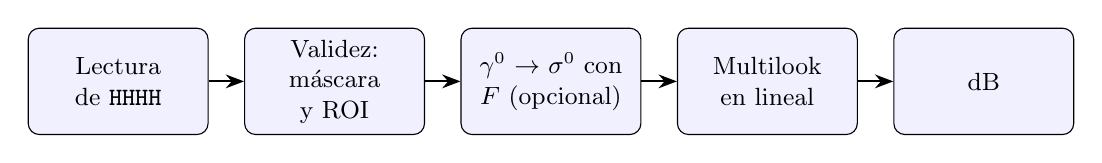
\begin{tikzpicture}[node distance=4.5mm,
  caja/.style={draw,rounded corners,fill=blue!6,align=center,text width=2.05cm,minimum height=1.35cm,font=\small},
  fl/.style={-{Stealth},thick}]
\node[caja] (a) {Lectura de \texttt{HHHH}};
\node[caja,right=of a] (b) {Validez: máscara y ROI};
\node[caja,right=of b] (c) {$\gamma^0\to\sigma^0$ con $F$ (opcional)};
\node[caja,right=of c] (d) {Multilook en lineal};
\node[caja,right=of d] (e) {dB};
\draw[fl] (a)--(b); \draw[fl] (b)--(c); \draw[fl] (c)--(d); \draw[fl] (d)--(e);
\end{tikzpicture}
\caption{El recorrido de un píxel: de la lectura a la escala en dB. El orden importa: el promedio se hace
\emph{antes} de pasar a decibeles.}
\label{fig:recorrido}
\end{figure}

\subsection{Paso 1: lectura}

El valor se lee directamente de la capa \texttt{HHHH} o \texttt{HVHV}. El programa no lo transforma: el
archivo ya trae potencia lineal en la convención $\gamma^0$. Supóngase, como ejemplo, que un píxel vale
$\gamma^0_{HH}=0.158$.

\subsection{Paso 2: validez}

Un píxel entra al análisis solo si su máscara no es 0 ni 255 y si cae dentro del polígono de la ROI
(sección~\ref{sec:figuras}). Si no cumple, se descarta como NaN y \emph{no} se sustituye por cero: un cero
significaría «sin retorno» y distorsionaría cualquier promedio. En la escena de la Etapa 1, El $99.61\,\mathrm{\%}$ de los
píxeles del polígono son válidos.

\subsection{Paso 3: de $\gamma^0$ a $\sigma^0$ (cuando se requiere)}

Con la capa del factor $F$ en ese mismo píxel (ejemplo ilustrativo: $F=0.74$),
\begin{equation}
  \sigma^0 = \gamma^0F = 0.158\times0.74 = 0.117 .
\end{equation}
En dB, $\gamma^0_{dB}=10\log_{10}0.158=-8.01$\,dB y $\sigma^0_{dB}=10\log_{10}0.117=-9.32$\,dB; la diferencia
$-1.31$\,dB es $10\log_{10}F$. El valor $F=0.74$ equivale a $\cos\theta$ con $\theta\approx42^\circ$,
razonable para esta geometría; en relieve fuerte, $F$ puede apartarse bastante.

\subsection{Paso 4: multilook en lineal}

Los píxeles de un bloque de $2\times2$ se promedian en lineal, con la regla de validez
$N_v\ge0.5\,n^2$ (figura~\ref{fig:multilook_bloques} y tabla~\ref{tab:bloques}). Promediar en lineal es
la operación físicamente coherente, porque la potencia (y no su logaritmo) es la cantidad que se suma.

\subsection{Paso 5: a decibeles}

Solo al final se calcula $10\log_{10}\bar P_B$. El resultado es el valor que se pinta en las figuras B y B2 y
que alimenta las estadísticas por región.

\begin{cuidado}
El orden «dB primero, promedio después» es un error muy frecuente. Produce un valor sistemáticamente menor
(el sesgo de Jensen de la sección~\ref{sec:speckle}) que además depende del número de looks, y por tanto no es
comparable entre productos con distinto procesamiento.
\end{cuidado}

\section{De un píxel a una región}
\label{sec:region}

Una cifra útil rara vez es la de un solo píxel. Para una región de interés se calculan estadísticas sobre
todos los píxeles válidos. En la escena de la Etapa 1, $n=14\,699\,442$ píxeles por polarización, a resolución
completa (sin multilook). La tabla~\ref{tab:stats-roi} reúne las estadísticas del histograma y las lee con
cuidado.

\begin{table}[htbp]
\centering\small
\begin{tabularx}{\linewidth}{p{.3\linewidth}rrX}
\toprule
\textbf{Estadística} & \textbf{HH} & \textbf{HV} & \textbf{Cómo leerla}\\\midrule
Media de los dB & $-8.055$ & $-13.503$ & Resume la distribución \emph{en dB}; no es una potencia media.\\
Mediana (dB) & $-7.880$ & $-13.173$ & Robusta frente a píxeles brillantes.\\
dB de la media lineal & $-3.786$ & $-9.226$ & Equivale a la potencia media real; sensible a colas brillantes.\\
Diferencia entre las dos medias & $4.27$ & $4.28$ & Mide la asimetría y el moteado, no un cambio.\\
$p_5$ a $p_{95}$ (dB) & $-14.07$ a $-2.85$ & $-20.00$ a $-8.11$ & Rango donde cae el 90\,\% central.\\
Desviación estándar (dB) & $3.59$ & $3.73$ & Mezcla de moteado y textura real.\\\bottomrule
\end{tabularx}
\caption{Estadísticas de $\gamma^0$ en dB para la ROI de la Etapa 1 (HH y HV, resolución completa). Valores
tomados de \texttt{metadatos.json} de la carpeta de figuras.}
\label{tab:stats-roi}
\end{table}

\paragraph{¿Qué media reportar?} Depende de la pregunta. Para describir cómo se ve la distribución, la media de
los dB o la mediana. Para balances de energía o comparaciones físicas entre fechas, el promedio \emph{lineal}.
Lo esencial es declarar cuál se usó, porque difieren en 4.3\,dB en esta escena.

\paragraph{Qué indica la diferencia entre HH y HV.} En esta ROI HV es unos 5.4\,dB menor que HH en la media de
los dB ($-13.50$ frente a $-8.06$). Es consistente con la expectativa general de que la polarización cruzada
devuelve menos que la co-polarizada en la mayoría de las superficies, y con la figura B, donde HV se ve más
oscura.

\section{Un ejemplo con dos fechas}
\label{sec:ej-dos-fechas}

Supóngase una región pequeña con dos fechas comparables, en la que un píxel pasa de $P_1=0.10$ a $P_2=0.20$
(potencias lineales). Entonces
\begin{equation}
  \Delta\sigma^0_{dB}=10\log_{10}\frac{0.20}{0.10}=+3.01\ \text{dB},
\end{equation}
una duplicación de potencia. ¿Es un cambio real? Depende del contexto estadístico:
\begin{itemize}
  \item Si cada fecha es de $L=1$ look, $\sigma_\Delta\approx7.9$\,dB y el resultado \emph{no} es distinguible
        del azar ($z\approx0.4$).
  \item Con $L=4$ (por ejemplo, un multilook $2\times2$ de píxeles independientes), $\sigma_\Delta\approx3.3$\,dB
        y $z\approx0.9$: tampoco.
  \item Si se promedian 100 píxeles independientes con $L=4$, $\sigma_\Delta\approx0.33$\,dB y la misma
        diferencia $3.01$\,dB es $z\approx9$: ahora sí es una señal clara \emph{de que la respuesta radar
        cambió}.
\end{itemize}
Lo que ningún caso responde es \emph{por qué} cambió. Esa pregunta pertenece a la interpretación, con los modelos
de la sección~\ref{sec:que-mide} y datos independientes.

\begin{atencion}
Un mapa de $\Delta\sigma^0$ con píxeles aislados de $\pm3$\,dB puede verse espectacular y no significar nada: es
lo que produce el moteado sin ningún cambio real (figura~\ref{fig:delta_distribucion}). Antes de interpretar
un mapa de cambio hay que preguntarse cuántos píxeles independientes sostienen cada conclusión.
\end{atencion}

\section{Una lista de comprobación antes de interpretar}
\label{sec:checklist-radar}

\begin{enumerate}
  \item ¿Las dos escenas son del mismo producto, trayectoria, marco, dirección, polarización, resolución,
        CRID y madurez?
  \item ¿La malla es idéntica y se verificó la cobertura de píxeles válidos en las dos fechas?
  \item ¿Se promedió en lineal antes de pasar a dB, con la misma regla de validez en ambas fechas?
  \item ¿Cuántos píxeles independientes sostienen la cifra y cuál es la dispersión esperada por moteado?
  \item ¿El umbral de «cambio importante» se fijó antes de ver el resultado y está registrado?
  \item ¿Se declara qué media (lineal o en dB) se reporta?
  \item ¿Se distingue en el texto entre lo observado, lo inferido y lo supuesto?
  \item ¿Hay un dato independiente (precipitación, imagen óptica, OPERA) que apoye o contradiga la hipótesis?
\end{enumerate}

\section{Contraste con fuentes independientes}
\label{sec:contraste}

Un $\Delta\sigma^0$ por sí solo no identifica su causa. Las fuentes auxiliares del proyecto aportan información
complementaria y cada una tiene un alcance distinto, como se resume en la tabla~\ref{tab:fuentes-aux}.

\begin{table}[htbp]
\centering\small
\begin{tabularx}{\linewidth}{p{.2\linewidth}p{.32\linewidth}X}
\toprule
\textbf{Fuente} & \textbf{Qué aporta} & \textbf{Qué limita}\\\midrule
GPM IMERG & Precipitación estimada por satélite en una malla gruesa, con alta frecuencia temporal. & Resolución espacial baja frente al píxel SAR; es una estimación, no lluvia medida en el sitio.\\
HLS (óptico) & Reflectancia en bandas visibles e infrarrojas, útil para vegetación y agua. & Depende de que haya cielo despejado el día de interés.\\
OPERA & Productos derivados de radar y óptico, entre ellos máscaras de agua y perturbación. & Sus propios supuestos y versiones; deben leerse con sus metadatos.\\\bottomrule
\end{tabularx}
\caption{Fuentes independientes para contrastar un cambio de respuesta radar.}
\label{tab:fuentes-aux}
\end{table}

El contraste útil es \emph{espacio-temporal}: compara el patrón y la fecha de lo que se ve en el radar con el
patrón y la fecha de lo que cuentan las otras fuentes, y reporta tanto coincidencias como discrepancias. Que
una lluvia intensa preceda un aumento de $\Delta\sigma^0$ es coherente con una hipótesis de humedad o
inundación, pero no la demuestra; una imagen óptica sin nubes que muestre agua en el mismo lugar la apoya más
fuertemente.

\section{Trazabilidad y reproducibilidad}
\label{sec:trazabilidad}

Cada cifra de la Etapa 1 se puede rastrear porque el flujo guarda, junto a cada resultado, \emph{de dónde} salió.
\begin{description}[style=nextline]
  \item[\texttt{metadatos.json}] Parámetros, estadísticas y la versión del código (\texttt{version\_codigo}) con
        que se generó la carpeta de figuras.
  \item[\texttt{control/*.csv}] Las tablas numéricas de las que salen las figuras; ningún número se calcula
        sobre los PNG.
  \item[Hashes y versión] Identificadores de las entradas y del código. Un sufijo \texttt{-dirty} en la
        versión indica cambios sin confirmar en el repositorio.
\end{description}
La nota sobre \texttt{98f7e07-dirty} de la sección~\ref{sec:figuras} no es un tecnicismo: significa que, para
citar las cifras en una publicación, conviene regenerar la carpeta con el árbol de \texttt{git} limpio, de
modo que cualquiera pueda reconstruir exactamente el mismo resultado.

\part{Simulación de inundación DG2 por región de interés}
\label{part:inundacion}

Se describe la ruta implementada que, a petición autenticada, transforma una región de interés (ROI) y un dominio declarados en un escenario de lluvia \emph{sintética}, prepara terreno NASADEM, ejecuta LISFLOOD-FP 8.0 DG2 CPU y ofrece mapas numéricos de profundidad. Se distinguen tres niveles: el modelo físico de aguas someras, su aproximación numérica DG2 y el adaptador de archivos, procesos y API. Cada ecuación identifica magnitudes y unidades; las afirmaciones de ejecución se vinculan al código. Un resultado integrable y descargable no es una predicción validada de inundación: todavía faltan una elección científicamente defendible del dominio, caudales, rugosidad, infiltración, balance comprobado y contraste independiente. No se atribuye a NISAR ninguna profundidad, lluvia ni causa de cambio.

\noindent\emph{Versión documental de la implementación observada en la rama} \texttt{simulacion-inundancion}.


\section{Guía conceptual: del agua en una celda al mapa de profundidad}
\label{sec:guia-inundacion}

Las secciones siguientes de esta parte son densas porque cada afirmación se vincula a una ecuación y a un
archivo de código. Esta sección ofrece, antes, el \emph{mapa del territorio}: qué problema físico se resuelve,
con qué idea numérica y qué ejemplo concreto produce una cifra que se puede verificar a mano. Quien lea solo
esta guía podrá seguir la lógica; quien después lea el resto podrá ubicar cada ecuación en ese mapa.

\subsection{El problema físico en una frase}

Cuando llueve sobre un terreno, el agua se acumula donde el relieve se lo permite y se mueve cuesta abajo,
frenada por la fricción del suelo. Si el agua es poco profunda comparada con la extensión horizontal que
recorre (una lámina de decenas de centímetros sobre cientos de metros), no hace falta resolver el movimiento
vertical: basta con seguir cuánta agua hay en cada punto, $h$, y con qué caudal por metro de ancho se desplaza,
$\mathbf q=(q_x,q_y)$. A este enfoque se le llama modelo de \textbf{aguas someras} (\emph{shallow water
equations}, SWE).

\subsection{Las dos leyes de conservación}

Las ecuaciones~\eqref{eq:conserv}--\eqref{eq:sources} dicen, en realidad, dos cosas muy cotidianas.
\begin{description}[style=nextline]
  \item[Conservación de la masa (primera componente).] El agua de una celda cambia solo porque entra, sale
        o cae lluvia sobre ella: $\partial_t h+\nabla\!\cdot\!\mathbf q=r$ (figura~\ref{fig:swe_celda}). Si no
        hay lluvia y todo el flujo que sale de una celda entra a la vecina, el volumen total no cambia.
  \item[Conservación de la cantidad de movimiento (segunda y tercera componentes).] El agua se acelera por la
        gravedad: la presión hidrostática empuja de zonas más profundas a menos profundas, y la pendiente del
        lecho tira cuesta abajo. La fricción con el fondo la frena, con una fuerza que crece con la rapidez.
\end{description}

\figura{swe_celda}{0.95}{Balance de masa en una celda de ancho $\Delta x$. La profundidad $h$ se mide desde el
lecho $z_b$ hasta la superficie libre $\eta=z_b+h$. El caudal por metro de ancho $q_x$ entra por un lado y sale
por el otro; la lluvia $r$ añade agua por arriba.}

\subsection{Lectura de cada término}

\begin{table}[htbp]
\centering\small
\begin{tabularx}{\linewidth}{p{.24\linewidth}p{.28\linewidth}X}
\toprule
\textbf{Término} & \textbf{Dónde aparece} & \textbf{Qué representa}\\\midrule
$\partial_t\boldsymbol U$ & Lado izquierdo & Cómo cambian en el tiempo la profundidad y el caudal.\\
$\partial_x\mathcal F+\partial_y\mathcal G$ & Lado izquierdo & Cuánto entra y sale por las caras de la celda (flujos).\\
$q_x^2/h$ & $\mathcal F$, componente 2 & Transporte de movimiento por el propio flujo (inercia).\\
$gh^2/2$ & $\mathcal F$, componente 2 & Presión hidrostática integrada en la columna.\\
$-gh\,\partial_xz_b$ & $\boldsymbol S_b$ & Fuerza de la gravedad sobre la pendiente del lecho.\\
$-ghS_{f,x}$ & $\boldsymbol S_f$ & Fricción de Manning con el fondo.\\
$r$ & $\boldsymbol S_r$ & Lluvia: añade profundidad, no momento.\\\bottomrule
\end{tabularx}
\caption{Traducción de cada término de la ecuación~\eqref{eq:conserv} a su significado físico.}
\label{tab:terminos-swe}
\end{table}

\subsection{La velocidad de las ondas y por qué importa}

En aguas someras, las perturbaciones viajan con la celeridad $c=\sqrt{gh}$ (además de ser arrastradas por la
corriente). Con $g=9.81$\,m/s$^2$: sobre $h=1$\,m las ondas viajan a $3.13$\,m/s; sobre $h=0.1$\,m, a $0.99$\,m/s;
sobre $h=1$\,cm, a $0.31$\,m/s. La consecuencia es directa: \emph{cuanto más profunda es el agua, más rápido
se propaga la información}, y el cálculo debe avanzar en pasos de tiempo más cortos para no «saltarse» una
onda de una celda a otra. Ese es el origen del límite CFL (sección~\ref{sec:dg2}).

\subsection{La idea del método: dividir el terreno en celdas}

Resolver las ecuaciones exactamente en cada punto es imposible; se divide el dominio en celdas rectangulares y
se calcula, en cada paso de tiempo, cuánta agua pasa por cada cara. El método clásico de \emph{volúmenes
finitos} guarda un solo número por celda (su valor medio). El método de Galerkin discontinuo de segundo orden
(DG2) que usa LISFLOOD-FP guarda \emph{tres} por cada campo: la media $W_0$ y dos pendientes $W_{1x}$, $W_{1y}$
que describen cómo varía el campo dentro de la celda (figura~\ref{fig:dg2_base}). Es como pasar de describir
cada celda con «una altura» a describirla con «una altura y una inclinación»: la superficie del agua puede
representarse con más fidelidad sin refinar la malla.

\figura{dg2_base}{0.7}{Representación modal en una celda (caso 1D). El campo real (gris) se aproxima con una
recta (azul); $W_0$ es la media y $W_{1x}$ controla la inclinación. Los valores en las caras son
$W_0\pm\sqrt{3}\,W_{1x}$ (círculos) y en los puntos de Gauss $W_0\pm W_{1x}$ (cuadrados).}

\subsection{Tres ingredientes numéricos, en lenguaje llano}

\paragraph{1. El flujo entre celdas (HLL).} En cada cara hay un estado a la izquierda y otro a la derecha. El
solver HLL (Harten--Lax--van Leer) estima cuánto agua y cuánto movimiento pasan por esa cara a partir de dos
velocidades de onda extremas, $S^-$ y $S^+$ (figura~\ref{fig:hll_abanico}). Es una aproximación robusta: no
resuelve toda la estructura de ondas, pero conserva la masa y no inventa valores negativos de profundidad en
casos usuales.

\figura{hll_abanico}{0.55}{Estructura del problema de Riemann aproximado en una cara. Dos ondas extremas
($S^-$ y $S^+$) separan el estado izquierdo $U_L$, un estado intermedio $U^*$ y el derecho $U_R$.}

\paragraph{2. El lecho y el borde seco (reconstrucción hidrostática).} Una pregunta esencial en inundaciones es
qué pasa en la orilla del agua, donde una celda está mojada y la vecina, más alta, está seca. Sin cuidado, el
método numérico produciría un flujo ficticio hacia el terreno seco o profundidades negativas. La
\emph{reconstrucción hidrostática} (figura~\ref{fig:reconstruccion_hidro}) iguala las dos caras a un mismo nivel
de referencia $z^*=\max(z_b^-,z_b^+)$ y calcula la profundidad efectiva $h^*=\max(0,\eta-z^*)$: si la
superficie del agua está por debajo de la cota del lecho vecino, el agua no puede pasar.

\figura{reconstruccion_hidro}{0.78}{Reconstrucción hidrostática en una cara. La celda izquierda está mojada; la
derecha, seca y con lecho más alto. La profundidad efectiva del lado derecho es $0$, de modo que no se genera
flujo hacia el terreno seco.}

\paragraph{3. El avance en el tiempo (RK2 y CFL).} El método avanza con dos etapas de Runge--Kutta y elige el
paso de tiempo para que ninguna onda cruce más de una fracción de celda (el \emph{número de Courant},
$C_{CFL}=0.33$ por defecto). La figura~\ref{fig:cfl_dt} muestra cómo el paso máximo cae al aumentar la
profundidad y la velocidad.

\figura{cfl_dt}{0.66}{Límite de estabilidad CFL para celdas de 20\,m con $C_{CFL}=0.33$. Con agua muy poco
profunda ($h=1$\,cm) el límite sería de $\approx21$\,s; con $h=1$\,m, de $2.1$\,s; con $h=0.1$\,m y corriente de
0.5\,m/s, de $4.4$\,s.}

\begin{ejemplo}[Un paso de tiempo calculado a mano]
Para $h=0.1$\,m, $|u|=0.5$\,m/s y $\Delta x=20$\,m:
\[
  \Delta t\le C_{CFL}\frac{\Delta x}{|u|+\sqrt{gh}}
  =0.33\,\frac{20}{0.5+\sqrt{9.81\times0.1}}
  =\frac{6.6}{0.5+0.990}=4.43\ \text{s}.
\]
En el caso del ejemplo de la solicitud (simulación de 2\,s con $\Delta t_{inicial}=0.1$\,s) el paso inicial ya
es más pequeño que ese límite, y manda la cota inferior de $\min(\Delta t_{inicial},\ldots)$.
\end{ejemplo}

\subsection{Fricción de Manning: una intuición}

El coeficiente de Manning $n_M$ resume qué tan áspera es la superficie: valores bajos (0.02) corresponden a
superficies lisas, y valores altos (0.08 o más) a vegetación densa. La fuerza de fricción crece con el
cuadrado de la rapidez y disminuye con la profundidad: cuanto menos agua hay, más domina el fondo sobre el
movimiento (figura~\ref{fig:manning_friccion}).

\figura{manning_friccion}{1.0}{Izquierda: coeficiente de fricción $C_f=gn_M^2/h^{1/3}$ en función de la
profundidad para tres valores de $n_M$. Derecha: pendiente de fricción con $u=1$\,m/s. Con el mismo $n_M$, la
fricción es mucho mayor en láminas delgadas.}

\begin{ejemplo}[Fricción en una lámina de 10\,cm]
Con $n_M=0.02$, $h=0.1$\,m y $u=1$\,m/s, el coeficiente es
$C_f=9.81\times0.02^2/0.1^{1/3}=0.00845$ y la pendiente de fricción,
$S_f=n_M^2u^2/h^{4/3}=0.0004/0.0464=0.0086$, es decir, unos $8.6$\,mm de pérdida de carga por cada metro de
recorrido.
\end{ejemplo}

\subsection{De una petición a un volumen: el ejemplo completo}
\label{sec:ej-lluvia}

El ejemplo de solicitud de la sección~\ref{sec:vida} permite seguir la lluvia hasta un volumen de agua.

\begin{enumerate}
  \item \textbf{Cantidad y duración.} $P=2$\,mm en $T_r=1$\,s. La tasa media es
        $\bar r=P/T_r=0.002$\,m/s, es decir, $0.002\times1000\times3600=7200$\,mm/h: matemáticamente coherente,
        físicamente extrema.
  \item \textbf{Intervalos.} Con $N=2$ intervalos de $0.5$\,s, la perturbación máxima es
        $\delta=\min(10\text{ mm/h},\bar r)=10\text{ mm/h}=2.78\times10^{-6}$\,m/s, despreciable frente a
        $\bar r$: las dos tasas son prácticamente iguales a $0.002$\,m/s.
  \item \textbf{Lámina por celda.} En cada centro de celda dentro de la ROI se suma $r_k\Delta t$ metros de
        profundidad; en total, $2$\,mm.
  \item \textbf{Volumen por celda.} Con celdas de $20$\,m, $\Delta A=400$\,m$^2$ y el volumen de lluvia por celda
        es $0.002\ \text{m}\times400\ \text{m}^2=0.8$\,m$^3$.
  \item \textbf{Volumen total.} Es $0.8$\,m$^3$ multiplicado por el número $N_{ROI}$ de centros dentro de la ROI.
        Con $N_{ROI}=4$ (valor ilustrativo), serían $3.2$\,m$^3$.
\end{enumerate}

\figura{malla_dominio}{0.78}{Esquema de la malla. La ROI (verde) y el dominio (azul discontinuo) se proyectan a un
CRS métrico; el rectángulo de cálculo (negro) añade dos celdas por lado. La lluvia solo se aplica en los
centros de celda (puntos verdes) que caen dentro de la ROI.}

\figura{lluvia_perfil}{0.7}{Perfil \texttt{uniform\_balanced} (ilustración con semilla arbitraria): 10
intervalos con tasas que oscilan alrededor de una media de 20\,mm/h, de modo que la suma de la lámina
coincide con los 20\,mm prescritos.}

\begin{intuicion}
El perfil \texttt{uniform\_balanced} existe para que la lluvia no sea perfectamente constante sin cambiar
el \emph{total}: las perturbaciones se generan en pares $\pm d$, así que se cancelan exactamente. La suma de
la lámina de los intervalos es la cantidad solicitada (ecuación~\eqref{eq:rainbal}); lo que el solver integre
con sus propios pasos requiere comprobación aparte.
\end{intuicion}

\subsection{Qué pregunta responde cada módulo}

\begin{table}[htbp]
\centering\small
\begin{tabularx}{\linewidth}{p{.25\linewidth}p{.28\linewidth}X}
\toprule
\textbf{Módulo} & \textbf{Pregunta} & \textbf{Respuesta que \emph{no} da}\\\midrule
Radar (Partes~\ref{part:fundamentos}--\ref{part:pixel}) & ¿Cambió la respuesta radar entre dos fechas? & La causa física del cambio.\\
Inundación (esta parte) & Si cayera esta lluvia hipotética, ¿qué láminas de agua resultan en este relieve? & Dónde \emph{realmente} se inundó; la predicción de un evento.\\
Solar (Parte~\ref{part:solar}) & ¿Cuánta irradiancia directa de cielo despejado incidiría sobre el terreno en este instante? & La radiación real con nubes, ni la difusa.\\\bottomrule
\end{tabularx}
\caption{Cada módulo responde una pregunta acotada. Confundirlas es la fuente de interpretaciones erróneas más
frecuente.}
\label{tab:modulos}
\end{table}


\section{Guía de lectura y alcance}
\label{sec:alcance}
\begin{center}
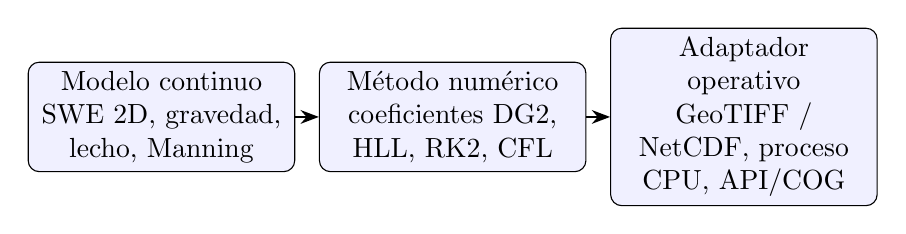
\begin{tikzpicture}[node distance=3mm,box/.style={draw,rounded corners,fill=blue!6,align=center,text width=3.15cm,minimum height=1.3cm},arr/.style={-{Stealth},thick}]
\node[box] (a) {Modelo continuo\\SWE 2D, gravedad, lecho, Manning};
\node[box,right=of a] (b) {Método numérico\\coeficientes DG2, HLL, RK2, CFL};
\node[box,right=of b] (c) {Adaptador operativo\\GeoTIFF / NetCDF, proceso CPU, API/COG};
\draw[arr] (a)--(b); \draw[arr] (b)--(c);
\end{tikzpicture}
\end{center}
\noindent\textbf{Pregunta y respuesta.} ¿Qué calcula la cadena disponible? La profundidad $h$ de una lámina superficial, en metros \emph{sobre el lecho local}, para un dominio métrico rectangular, bajo lluvia hipotética espacialmente uniforme en las celdas seleccionadas por la ROI, estado inicial seco, Manning constante y borde idealizado elegido. Los mapas muestran profundidades de cuadros y máximo; no son mapas medidos por satélite. El cálculo no proporciona al cliente velocidad, tiempo de llegada ni extensión observada. El usuario elige entradas y supuestos; el servicio no determina si son físicamente correctos.

El escenario se limita a terreno declarado no urbano. \texttt{domain\_nonurban:true} expresa una declaración del solicitante, no una clasificación automática de cobertura del suelo. Una ROI de consulta no delimita necesariamente la cuenca que alimenta el flujo; el dominio debe contemplar aportes y salidas. Aquí no se representan calles, alcantarillas, edificios, batimetría detallada ni flujo subterráneo. Si esas omisiones controlan el evento, no interpretar el resultado como una simulación regional válida. La ruta ROI actual es \src{pipeline/hydrology/roi_runner.py}; los casos registrados y \texttt{prepare/} son contratos diferentes y no se mezclan.

\warn{La verificación de formato y de ejecución no equivale a validación hidráulica. Los valores numéricos de una solicitud de ejemplo más adelante son únicamente ilustrativos; no son recomendaciones ni resultados observados.}

\section{Magnitudes, referencias y supuestos físicos}
\label{sec:simbolos}
Se suponen coordenadas horizontales proyectadas $x,y$ en metros (no grados), tiempo $t$ en segundos desde el comienzo \emph{simulado} y lecho estacionario $z_b(x,y)$ en metros de elevación respecto de un datum vertical declarado. $h(x,y,t)\geq0$ es altura de agua \emph{sobre ese lecho}, no altitud absoluta. La superficie libre $\eta=z_b+h$ es elevación respecto del \emph{mismo} datum; restar cotas de datum diferente no produce una profundidad. NASADEM\_HGT aporta elevación referida al geoide EGM96; la reproyección horizontal no efectúa una conversión vertical. $u,v$ son componentes de velocidad horizontal \emph{promediadas en la profundidad}, en m/s; $g$ es aceleración gravitatoria en m/s$^2$.

Definimos $q_x=hu$ y $q_y=hv$ (m$^2$/s): cada uno es volumen que cruza una sección vertical \emph{por segundo y por metro de ancho perpendicular}. En cambio $Q=\int_B\boldsymbol q\cdot\boldsymbol n_{\!f}\,\dd\ell$ tiene m$^3$/s a través del ancho $B$ de una frontera/sección; $\boldsymbol n_{\!f}$ es la normal horizontal unitaria, no la rugosidad de Manning $n_M$. Para flujo uniforme sobre ancho $B$, $Q=q_{\perp}B$, pero no para una sección heterogénea. $Q/A_c$ (m/s) divide por área \emph{transversal mojada} $A_c$ (m$^2$), velocidad media; $Q/A_p$ (m/s) divide por área \emph{horizontal en planta} $A_p$ (m$^2$), tasa areal equivalente únicamente si se distribuye allí el volumen. El símbolo $q_s$ designará exclusivamente otra \emph{fuente areal} de profundidad (m/s), nunca $q_x$ o $Q$. No hay entrada $q_s$ general en esta API.

\begin{longtable}{p{.18\linewidth}p{.17\linewidth}p{.57\linewidth}}
\toprule Símbolo & Unidad SI & Referencia, denominador o interpretación\\\midrule\endhead
$h,z_b,\eta$ & m & Profundidad desde lecho; cota de lecho y cota de superficie libre desde datum común. $\eta-z_b=h$.\\
$x,y,\Delta x,\Delta y$ & m & Posición horizontal y longitud de lado de celda proyectada; las diferencias no se miden en grados de latitud.\\
$t,\Delta t$ & s & Tiempo desde origen simulado y duración de un paso; sin fecha UTC inferida.\\
$u,v,c=\sqrt{gh}$ & m/s & Velocidad media de columna y celeridad gravitatoria; $gh$ tiene m$^2$/s$^2$.\\
$q_x,q_y$ & m$^2$/s & Caudal \emph{por unidad de ancho} de sección vertical, no m$^3$/s ni profundidad por tiempo.\\
$Q$ & m$^3$/s & Volumen por segundo a través de sección completa.\\
$r,i,q_s$ & m/s & Lámina ganada por lluvia, perdida por infiltración y fuente neta por \emph{área horizontal y tiempo}: m$^3$/(m$^2$ s). $i,q_s$ son conceptuales, no aplicados por la ruta ROI.\\
$n_M$ & s/m$^{1/3}$ & Coeficiente Manning en la convención SI del solver, no una normal ni un conteo; valor requerido explícito en solicitud.\\
$S_{f,x},S_{f,y}$ & 1 & Pérdida de altura de energía por longitud horizontal (m/m), pendiente de fricción con signo de velocidad.\\
$\mathcal F,\mathcal G$ & (m$^2$/s, m$^3$/s$^2$, m$^3$/s$^2$) & Primera componente flujo de masa/profundidad por ancho; otras dos, flujos de momento integrado en la columna por longitud de borde y tiempo.\\
$\Delta A=\Delta x\Delta y$ & m$^2$ & Área horizontal de una celda, usada para convertir lámina a volumen.\\\bottomrule
\end{longtable}

El modelo de aguas someras integra verticalmente, supone presión aproximadamente hidrostática y representa escala horizontal mucho mayor que la profundidad característica. No resuelve velocidad vertical ni turbulencia local 3D. El lecho puede ser especialmente incierto bajo agua, vegetación, puentes y cauces estrechos: refinar una malla remuestreada no crea topografía ausente.

\section{Ecuaciones continuas y conservación}
\label{sec:ecuaciones}
Para $\boldsymbol U=(h,q_x,q_y)^{\mathrm T}$, la forma conservativa bidimensional del modelo base es
\begin{align}
\partial_t\boldsymbol U+\partial_x\mathcal F(\boldsymbol U)+\partial_y\mathcal G(\boldsymbol U)&=\boldsymbol S_b+\boldsymbol S_f+\boldsymbol S_r,\label{eq:conserv}\\
\mathcal F&=\begin{pmatrix}q_x\\ q_x^2/h+gh^2/2\\q_xq_y/h\end{pmatrix},\qquad
\mathcal G=\begin{pmatrix}q_y\\q_xq_y/h\\q_y^2/h+gh^2/2\end{pmatrix},\label{eq:flux}\\
\boldsymbol S_b&=\begin{pmatrix}0\\-gh\partial_xz_b\\-gh\partial_yz_b\end{pmatrix},\quad
\boldsymbol S_r=\begin{pmatrix}r\\0\\0\end{pmatrix},\quad
\boldsymbol S_f=\begin{pmatrix}0\\-ghS_{f,x}\\-ghS_{f,y}\end{pmatrix}.\label{eq:sources}
\end{align}
En $h=0$, los cocientes en \eqref{eq:flux} no se evalúan directamente: el código aplica umbrales y reconstrucción de caras. La escritura continua representa la física \emph{idealizada}; no reproduce por sí misma la secuencia discreta de operadores. La lluvia se añade a profundidad y no aporta momento explícito en la ruta DG2 consultada. Generalmente podría escribirse $\partial_t h+\nabla\cdot\boldsymbol q=r-i+q_s$, con términos de momento asociados a intercambios de masa si corresponde; \textbf{aquí} no se invocan infiltración ni fuente areal adicional mediante la API, por lo que en el interior el aporte externo implementado es $r$. No atribuir soporte físico a opciones que el parser nativo pudiera reconocer sin que el bucle DG2 las aplique.

\subsection{Comprobación dimensional término por término}
En continuidad, $[\partial_t h]=\unit{m/s}$ y $[\partial_xq_x]=[\partial_yq_y]=(\unit{m^2/s})/\unit m=\unit{m/s}$. La precipitación $r$ se define por \emph{área de planta}, de modo que $r\Delta A\Delta t$ es m$^3$. Ninguna intensidad en mm/h puede sumarse directamente a $h$ en m sin convertirla y multiplicarla por segundos.

En cada componente de momento, $[\partial_t q_x]=\unit{m^2/s^2}$. $[q_x^2/h]=(\unit{m^2/s})^2/\unit m=\unit{m^3/s^2}$ y $[gh^2]=\unit{m^3/s^2}$; las derivadas $\partial_x,\partial_y$ dividen por distancia horizontal, dando m$^2$/s$^2$. El gradiente $\partial_xz_b$ compara metros verticales entre metros horizontales (adimensional); por tanto $[gh\partial_xz_b]=\unit{m^2/s^2}$. También $[gh S_{f,x}]=\unit{m^2/s^2}$ porque $S_{f,x}$ es pendiente adimensional. Un flujo de momento que cruza una cara, multiplicado por longitud de esa cara, tiene m$^4$/s$^2$; al dividir por el área de celda m$^2$ vuelve a m$^2$/s$^2$. Las identidades dimensionales no prueban ni exactitud de DEM ni conservación del programa.

\subsection{Manning, pendiente y operador efectivamente aplicado}
Con $w=\sqrt{u^2+v^2}$ (m/s), la convención continua de pendiente de fricción es
\begin{equation}
 S_{f,x}=\frac{n_M^2uw}{h^{4/3}},\quad S_{f,y}=\frac{n_M^2vw}{h^{4/3}},\qquad
 \boldsymbol S_{f,\mathrm{mom}}=-\frac{g n_M^2}{h^{1/3}}(uw,vw)^{\mathrm T}.\label{eq:mann}
\end{equation}
\[
[n_M^2uw/h^{4/3}]=(\unit{s^2/m^{2/3}})(\unit{m^2/s^2})/\unit{m^{4/3}}=1.
\] El factor $C_f=gn_M^2/h^{1/3}$ es adimensional: \[
(\unit{m/s^2})(\unit{s^2/m^{2/3}})/\unit{m^{1/3}}=1.
\] $C_fuw$ tiene m$^2$/s$^2$, \emph{no} es la pendiente adimensional $S_{f,x}$. En el código \src{swe/dg2/friction.cpp} se llama \texttt{Sfx} al término de momento negativo, no a la pendiente de energía definida en \eqref{eq:mann}. Usar una sola nomenclatura sin esta distinción daría ecuaciones incompatibles.

Para las medias y, cuando aplica, valores en puntos de Gauss, el método nativo calcula
\begin{align}
 C_f&=gn_M^2/h^{1/3}, & D_x&=1+\Delta t\frac{C_f}{h}\frac{2u^2+v^2}{w},
 & D_y&=1+\Delta t\frac{C_f}{h}\frac{u^2+2v^2}{w},\label{eq:fricden}\\
 q_x^{\mathrm{nuevo}}&=q_x+\Delta t\frac{-C_fuw}{D_x}, &
 q_y^{\mathrm{nuevo}}&=q_y+\Delta t\frac{-C_fvw}{D_y}.\label{eq:fricdisc}
\end{align}
$[\Delta t(C_f/h)(u^2/w)]=\unit s(1/\unit m)(\unit{m/s})=1$, así que $D_x,D_y$ son adimensionales. Los términos añadidos a $q_x,q_y$ tienen $(\unit s)(\unit{m^2/s^2})=\unit{m^2/s}$. El código evita dividir cuando $h\leq$ \texttt{DepthThresh} o ambas componentes de velocidad son menores que \texttt{SpeedThresh}; actualiza también coeficientes de pendiente desde evaluaciones en Gauss. \textbf{Este operador se aplica fuera de las dos etapas RK}; la presencia de RK2 no demuestra segundo orden temporal global con lluvia y fricción partidas. Referencia: \src{runtime/source/swe/dg2/friction.cpp}, funciones \texttt{apply\_friction} y \texttt{friction}; en adelante se abrevia \texttt{runtime/source} como \texttt{fuente nativa}.

\section{De la ecuación a DG2}
\label{sec:dg2}
\subsection{Representación modal y terreno}
Sea $K_{ij}$ una celda de lado $\Delta x,\Delta y$, centro $(x_i,y_j)$ y coordenadas locales $\xi=2(x-x_i)/\Delta x$, $\zeta=2(y-y_j)/\Delta y$, ambas entre $-1$ y $1$ y \emph{adimensionales}. No se usa $\eta$ para referencia espacial: $\eta$ ya es la superficie libre. La aproximación planar para cada campo $W\in\{h,q_x,q_y,z_b\}$ es
\begin{equation}
 W_h(x,y)=W_0+\sqrt3 W_{1x}\xi+\sqrt3 W_{1y}\zeta.\label{eq:basis}
\end{equation}
$W_0$ representa la media de celda y $W_{1x},W_{1y}$ amplitudes modales con \emph{las mismas unidades que $W$}; no son $\partial_xW,\partial_yW$ en unidades por metro. En efecto $\partial_xW_h=2\sqrt3W_{1x}/\Delta x$. Esta base da valores en las caras $W_0\pm\sqrt3W_{1x}$ y en las posiciones de Gauss de un eje $W_0\pm W_{1x}$. Los índices $1x,1y$ se refieren a los grados de libertad, no a bandas satelitales. El código \src{swe/dg2/modifiedvars.cpp} define \texttt{limit\_neg/pos} y \texttt{gauss\_lower/upper} con esas combinaciones; \src{swe/dg2.cpp} actualiza los nueve coeficientes de $h,q_x,q_y$ en cada paso.

El preprocesador oficial \texttt{generateDG2DEM} toma el raster \texttt{terrain.dem.raw} como muestras de vértice (con índices en el borde acotados a la última celda). Si NW, NE, SW y SE son las cuatro muestras de un elemento, su proyección implementada es
\begin{equation}
 z_0=\frac{NW+NE+SW+SE}{4},\quad
 z_{1x}=\frac{NE+SE-NW-SW}{4\sqrt3},\quad
 z_{1y}=\frac{NE+NW-SE-SW}{4\sqrt3}.\label{eq:vertices}
\end{equation}
Si NW y NE son iguales y SW y SE menores, $z_{1y}>0$ al tomar $y$ creciente hacia el norte. Todas estas magnitudes tienen metros EGM96: dividir por $\Delta x$ o $\Delta y$ para formar un gradiente cambia la unidad. La media DG2 puede diferir del valor original de una muestra DEM; no declarar que el asistente conserva cada pixel sin cambios. El adaptador rechaza huecos y los centinelas $-9999$ y $10^{10}$; el parámetro \texttt{nodata\_elevation 10000000000} evita confundir elevación cero con nodata en la utilidad. Véanse \src{preprocess/generateDG2DEM.cpp}, \src{swe/dg2/fields.cpp} (\texttt{initialise\_field}) y \src{pipeline/hydrology/dem_dg2.py}.

\subsection{Residuos, caras y lecho}
La formulación DG proyecta el balance sobre $1,\sqrt3\xi,\sqrt3\zeta$. Esquemáticamente, para cada función base $\phi_a$ y componente conservada, la forma débil por celda es
\begin{equation}
 \int_K \phi_a\,\partial_t U_h\,\dd A =
 \int_K\!\bigl(\mathcal F(U_h)\partial_x\phi_a+\mathcal G(U_h)\partial_y\phi_a+\phi_a S_b\bigr)\dd A
 -\int_{\partial K}\!\phi_a\widehat{\mathcal H}(U_h^-,U_h^+;\boldsymbol n_{\!f})\dd\ell.
 \label{eq:weak}
\end{equation}
Esta es una \emph{explicación matemática} de proyección, no una transcripción literal de cada bucle; el código evalúa flujos en caras y Gauss, reconstruye el lecho y calcula \texttt{L0}, \texttt{L1x}, \texttt{L1y}. Para el modo medio de profundidad, la ecuación de actualización sin lluvia dentro de $L$ es
\begin{equation}
 L_0(h)=-\frac{\widehat F^h_E-\widehat F^h_W}{\Delta x}
          -\frac{\widehat G^h_N-\widehat G^h_S}{\Delta y}.\label{eq:mean}
\end{equation}
En $x$ o $y$, $[\widehat F^h]=\unit{m^2/s}$; al dividir por m el residuo tiene m/s. Los modos lineales no se obtienen copiando \eqref{eq:mean}: \texttt{L1x/L1y} incluyen flujos físicos en los dos puntos de Gauss, contribuciones de caras y el término de lecho correspondiente al momento. Cuando \texttt{thin\_depth} se cumple, los incrementos lineales se anulan en \texttt{L}. Por eso describir el ejecutable como un volumen finito de solo media sería inexacto. El lecho entra como $-gh\nabla z_b$ con reconstrucción propia, no mediante una resta de alturas en un PNG.

En una cara entre reconstrucciones izquierda y derecha, \src{swe/dg2/modifiedvars.cpp} calcula $z^*=\max(z_b^-,z_b^+)$ y, para cada lado, $h^*=\max(0,\eta^{\pm}-z^*)$; si la profundidad original es suficientemente húmeda, $q^*=h^*(q/h)$, en caso contrario $q^*=0$. Esta reconstrucción hidroestática da sentido a estados de cara secos y busca coherencia con el equilibrio de lago en reposo, pero \emph{no demuestra} conservación exacta, positividad global ni balance bien equilibrado en este caso sin ensayos. Los términos \texttt{bed\_source\_0x/0y/1x/1y} de \src{swe/dg2.cpp} acompañan los flujos en la actualización modal.

\subsection{HLL y componente transversal}
Para cada cara, se resuelve aproximadamente un problema normal 1D con los estados reconstruidos y las componentes de \eqref{eq:flux}. Si $S^-<0<S^+$, las dos primeras componentes del flujo HLL corresponden a
\begin{equation}
 \widehat F_{\mathrm{HLL}}^{(h,q_\perp)}=
 \frac{S^+F_L^{(h,q_\perp)}-S^-F_R^{(h,q_\perp)}
       +S^-S^+(U_R-U_L)^{(h,q_\perp)}}{S^+-S^-}.\label{eq:hll}
\end{equation}
Si $S^-\geq0$ se toma $F_L$; si $S^+<0$, $F_R$. $S^{\pm}$ son velocidades de ondas en m/s, acotadas en la fuente con $u\pm\sqrt{gh}$ y estimadores intermedios, con ramas especiales para estados secos. En la rama intermedia, \emph{la componente transversal no se calcula simplemente aplicando \eqref{eq:hll} a las tres componentes}: el código determina una onda de contacto intermedia y usa el flujo de profundidad central multiplicado por la velocidad transversal del lado elegido. La rutina en $y$ intercambia las componentes normales y transversales. Esto importa al comparar una ecuación HLL de libro con \src{swe/hll_include.h} y \src{swe/flux.cpp}. Chequeo: $[S^-S^+(h_R-h_L)]=\unit{(m/s)^2m}=\unit{m^3/s^2}$ y al dividir por $S^+-S^-$ (m/s) da m$^2$/s, como el flujo de profundidad; para momento, $(\unit{m/s})^2(\unit{m^2/s})/(\unit{m/s})=\unit{m^3/s^2}$.

\subsection{Dos etapas temporales y restricciones de estabilidad}
Al llamar $L$ al vector de residuos de los nueve coeficientes (con flujo y lecho), el núcleo ejecuta
\begin{equation}
 U^{(1)}=U^n+\Delta t L(U^n),\qquad
 U^{n+1}=\tfrac12\bigl(U^n+U^{(1)}+\Delta t L(U^{(1)})\bigr).\label{eq:rk}
\end{equation}
Es RK de dos etapas para \emph{ese} residuo: no se debe atribuir automáticamente segundo orden temporal al acoplamiento completo. \src{swe/dg2.cpp} aplica lluvia, actualiza condiciones, opcionalmente recalcula $\Delta t$, aplica fricción y luego \texttt{rk\_stage1/rk\_stage2}; a continuación actualiza máximos, acumula estadísticas de flujo, incrementa $t$ y escribe cuando se alcanzan los umbrales de guardado. No hay llamada a infiltración en \texttt{dg2::solve}. La aplicación de lluvia precede incluso al recálculo CFL: al iniciar un ciclo usa el \texttt{Tstep} vigente para $h\mathrel{+}=r\Delta t$ y después, si el modo adaptativo está activado, puede sustituir ese paso. Es un detalle de orden real que exige revisar balance con datos de ejecución; no se supone conservación exacta ni error cuantificado sin medirlo.

Cuando se habilita \texttt{adaptive\_ts}, la regla nativa de cada estado húmedo y borde es
\begin{equation}
 \Delta t\leq\min\!\left(\Delta t_{\mathrm{inicial}},
 C_{\mathrm{CFL}}\frac{\Delta x}{|u|+\sqrt{gh}},
 C_{\mathrm{CFL}}\frac{\Delta y}{|v|+\sqrt{gh}}\right).\label{eq:cfl}
\end{equation}
Las fracciones tienen segundos: m/(m/s). \texttt{dg2} fija por defecto $C_{\mathrm{CFL}}=0.33$, \texttt{DepthThresh}=0.001\,m, \texttt{DG2DepthThresh}=$-1$ y \texttt{DG2ThinDepthTstep}=0; un paso delgado positivo configurado puede imponer otra cota. \texttt{SpeedThresh} se inicializa en la fuente nativa para evitar operaciones con velocidades minúsculas. Los umbrales son mecanismos internos, \emph{no} tolerancias de error físico aprobadas. \src{lisflood.cpp} inicia \texttt{adaptive\_ts=ON}; el archivo \texttt{.par} de esta ruta declara \texttt{initial\_tstep}, pero no contiene opción que cambie explícitamente esa bandera. Por tanto, el camino normal usa recálculo CFL según ese default nativo, sujeto a comprobar la configuración efectiva de cada ejecución; no atribuir el modo adaptativo únicamente a \texttt{initial\_tstep}. El limitador de pendientes existe (Krivodonova/minmod en \src{swe/dg2/slope_limiter.cpp}) pero \texttt{limit\_slopes} inicia desactivado y la ruta ROI no lo activa; los bordes tienen tratamiento propio. Ningún umbral implica precisión, estabilidad o resolución de frente demostrada. Fuentes: \src{pars.cpp} (opción \texttt{dg2}), \src{lisflood.cpp} (inicialización), \src{swe/dg2.cpp} (\texttt{Tstep\_from\_cfl}, \texttt{min\_dt}, \texttt{solve}).

\section{Lluvia sintética: de la petición a un volumen}
\label{sec:lluvia}
La solicitud acepta cantidad acumulada $P$ y duración $T_r$ o intensidad y duración; \src{pipeline/hydrology/inputs.py} normaliza ambos modos a $P$ en m, $T_r$ en s y media $\bar r=P/T_r$ en m/s. Una intensidad expresada en mm/h se convierte con $r_{\mathrm{m/s}}=r_{\mathrm{mm/h}}/(1000\cdot3600)$. Cantidad en mm \emph{no} equivale a intensidad en mm/h hasta dividir por su intervalo temporal. La lluvia es definida por el usuario, no observada ni estimada a partir de radar.

Con número \emph{par} $N$ de intervalos iguales, $\Delta t_r=T_r/N$, el perfil \texttt{uniform\_balanced} genera $N/2$ desviaciones $d_j\sim\mathcal U[-\delta,\delta]$, sus opuestas $-d_j$, y reordena las $N$ contribuciones mediante semilla; aquí $\delta=\min(10/1000/3600\ \unit{m/s},\bar r)$. Luego $r_k=\bar r+d_k\geq0$ y
\begin{equation}
 \sum_{k=0}^{N-1}r_k\Delta t_r
 =N\bar r\frac{T_r}{N}+\Delta t_r\sum_kd_k=P.\label{eq:rainbal}
\end{equation}
Esta igualdad nominal conserva la lámina prescrita del \emph{perfil}; la integración real del solver con pasos propios y redondeos requiere comprobación separada. La cota solicitada $10$\,mm/h es límite de perturbación, no lluvia máxima: si la media es menor, la cota efectiva es menor; la lluvia instantánea puede superar la media. La misma tasa de cada intervalo se aplica a todos los \emph{centros de celda} dentro de la ROI; fuera es cero. La selección por centro es una discretización, no un campo meteorológico observado continuo. Si cada centro seleccionado tiene área $\Delta A$, el volumen nominal del intervalo es $V_k=r_k\Delta t_r N_{\mathrm{ROI}}\Delta A$, con m$^3$; para ROI recortada geométricamente no equiparar necesariamente $N_{\mathrm{ROI}}\Delta A$ a su área exacta. Véanse \src{pipeline/hydrology/rainfall.py} y \src{pipeline/hydrology/rainfall_netcdf.py}.

El exportador escribe NetCDF3 de desplazamiento de 64 bits, cubo \texttt{rainfall\_depth(time,y,x)} con \emph{mm acumulados por intervalo siguiente}, no m/s: $R_k=1000r_k\Delta t_r$. El eje \texttt{time} son horas desde cero, $x,y$ centros en metros, $x$ creciente y $y$ descendente; añade cuadro de lluvia nula al final y otro al término de la simulación si hay cola seca. El lector nativo \src{rain/rain.tpp} convierte el acumulado a tasa mediante
\begin{equation}
 r_k=\frac{R_k}{1000\,[3600(t_{k+1}^{\rm h}-t_k^{\rm h})]}\quad\unit{m/s},
 \qquad \Delta h=r_k\Delta t.\label{eq:ncrain}
\end{equation}
Para la contabilidad interna añade $\Delta V=\Delta h\Delta A$ por celda. El lector \src{lisflood2/file_tool.cpp} usa identificadores de variables como identificadores de dimensiones al consultar longitudes: el exportador establece deliberadamente el orden del encabezado y un eje ancla para compatibilidad con SciPy y \emph{esta versión} nativa. No generalizar el orden de variables a NetCDF arbitrarios ni atribuirle validez física. El lector usa horas por construcción, no interpreta libremente atributos alternativos de tiempo. La duración total debe cubrir la lluvia y su cola; la serie nula evita extender tácitamente la última tasa.

\section{Terreno, dominio, contorno e inicio}
\label{sec:entradas}
\subsection{De NASADEM a la malla de cálculo}
La ROI y \texttt{domain} llegan como polígonos EPSG:4326; el dominio debe cubrir la ROI. Tras proyectarlos a un CRS métrico válido elegido por la persona solicitante (por ejemplo, EPSG:32615 solo si es apropiado para el lugar), \src{pipeline/hydrology/roi_runner.py} alinea la caja de contorno a múltiplos de resolución, expande dos celdas por lado y obtiene un \emph{rectángulo completo}. No se simula solo el recorte poligonal: los bordes hidráulicos están en el rectángulo. El contorno inverso densificado determina teselas a adquirir. Se rechazan longitudes que crucen el antimeridiano y dominios fuera de latitudes NASADEM $-56^\circ$ a $60^\circ$; una tesela que simplemente intersecta la ROI no garantiza cobertura de toda la malla.

\src{pipeline/elevation/nasadem.py} adquiere HGT, \src{pipeline/hydrology/dem_prepared.py} prepara elevaciones y \texttt{roi\_runner} remuestrea la rejilla preparada a cada centro de la malla alineada. Se rechaza cualquier centro sin elevación finita; no se sustituye nodata por cero ni se inventa terreno. La operación vertical declarada conserva cotas EGM96: solo se reproyecta \emph{horizontalmente}. Los HGT de un segundo de arco son muestras angulares, no resolución métrica fija; el método \texttt{nearest} o \texttt{bilinear} solicitado no crea microtopografía. La idoneidad de cauces, diques naturales, vegetación, fecha y datum de niveles externos requiere estudio adicional. \texttt{prepare\_dg2\_dem} genera las tres capas modales \texttt{.dem}, \texttt{.dem1x}, \texttt{.dem1y}, con checks de geometría y hashes, sin certificar calidad topográfica.

\subsection{Frontera idealizada y condición inicial}
\texttt{dry\_zero\_velocity} implica $h(x,y,0)=q_x(x,y,0)=q_y(x,y,0)=0$ en el dominio: hipótesis impuesta, no prueba de que cauces, humedales o agua permanente estén secos. Sin \texttt{bcifile} el borde nativo por defecto es \texttt{NONE} (tratamiento reflectante de momento normal); con \texttt{boundary:free}, \src{pipeline/hydrology/boundaries.py} escribe \texttt{FREE} sobre los cuatro lados completos. En \src{swe/dg2.cpp}, \texttt{set\_boundary\_values}, \texttt{NONE} invierte la componente de momento normal fuera y \texttt{FREE} mantiene estado exterior igual a la media interior: \texttt{FREE} puede permitir entrada o salida según el estado; \emph{no} es la identificación observada de un desagüe ni una condición de nivel medida. La elección incorrecta del contorno puede dominar más que el orden numérico. La ruta ROI no acepta hidrograma de entrada, nivel observado ni batimetría como campos de su solicitud. Tampoco aplica infiltración: \texttt{infiltration:"unsupported"} reconoce una limitación, no un parámetro físico de pérdida igual a cero obtenido de medidas.

\section{Ciclo de vida operativo y API}
\label{sec:vida}
\begin{center}
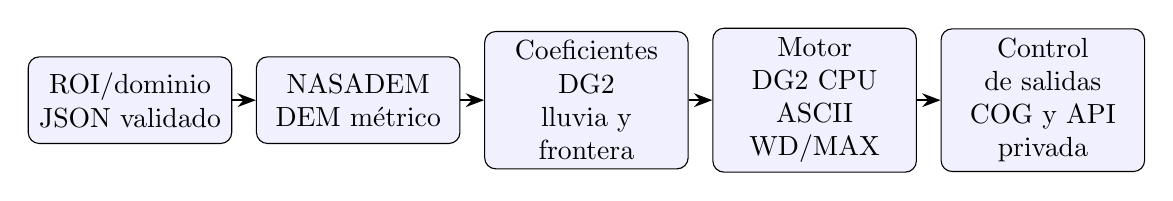
\begin{tikzpicture}[node distance=3mm,box/.style={draw,rounded corners,fill=blue!6,align=center,text width=2.35cm,minimum height=1.1cm},arr/.style={-{Stealth},thick}]
\node[box] (r) {ROI/dominio\\JSON validado};
\node[box,right=of r] (d) {NASADEM\\DEM métrico};
\node[box,right=of d] (f) {Coeficientes DG2\\lluvia y frontera};
\node[box,right=of f] (s) {Motor DG2 CPU\\ASCII WD/MAX};
\node[box,right=of s] (c) {Control de salidas\\COG y API privada};
\draw[arr] (r)--(d);\draw[arr] (d)--(f);\draw[arr] (f)--(s);\draw[arr] (s)--(c);
\end{tikzpicture}
\end{center}

\subsection{Diagrama A: de la solicitud al mapa descargable}
\label{sec:flujo-api}
El recorrido siguiente separa la \emph{admisión} (1--3), la \emph{preparación} (4--6), el \emph{cálculo} (7) y la \emph{publicación} (8--9). Cada caja indica entrada $\to$ transformación $\to$ salida; las ramas laterales son fallos, no resultados parciales publicables. El diagrama B abre la caja 7.
\begin{center}
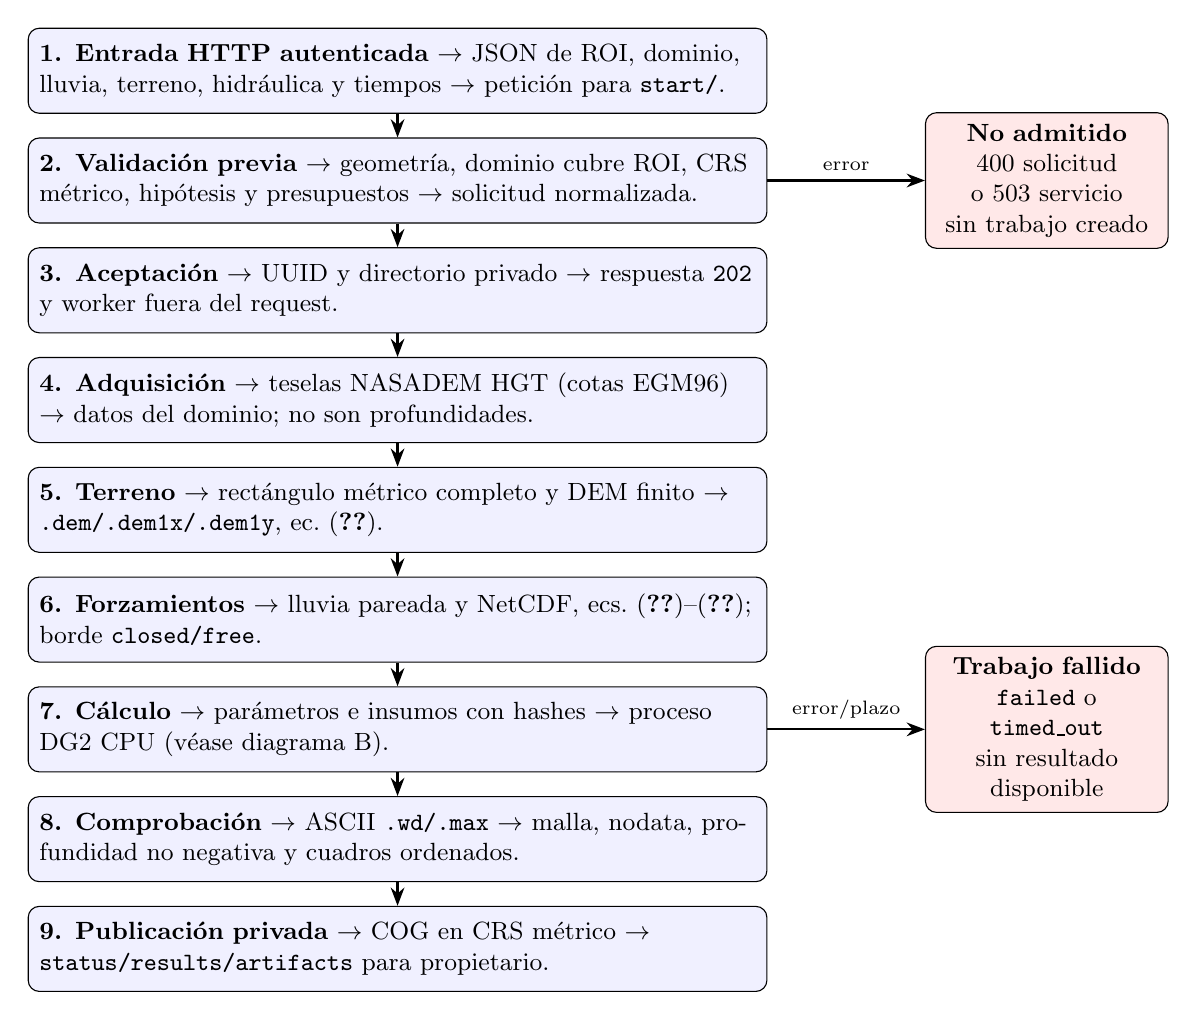
\begin{tikzpicture}[
 node distance=3mm,
 paso/.style={draw,rounded corners,fill=blue!6,align=left,text width=9.1cm,
              minimum height=1.08cm,inner sep=4pt,font=\small},
 fallo/.style={draw,rounded corners,fill=red!9,align=center,text width=2.8cm,
               inner sep=4pt,font=\small},
 flecha/.style={-{Stealth},thick}]
\node[paso] (a1) {\textbf{1. Entrada HTTP autenticada} $\to$ JSON de ROI, dominio, lluvia, terreno, hidráulica y tiempos $\to$ petición para \texttt{start/}.};
\node[paso,below=of a1] (a2) {\textbf{2. Validación previa} $\to$ geometría, dominio cubre ROI, CRS métrico, hipótesis y presupuestos $\to$ solicitud normalizada.};
\node[paso,below=of a2] (a3) {\textbf{3. Aceptación} $\to$ UUID y directorio privado $\to$ respuesta \texttt{202} y worker fuera del request.};
\node[paso,below=of a3] (a4) {\textbf{4. Adquisición} $\to$ teselas NASADEM HGT (cotas EGM96) $\to$ datos del dominio; no son profundidades.};
\node[paso,below=of a4] (a5) {\textbf{5. Terreno} $\to$ rectángulo métrico completo y DEM finito $\to$ \texttt{.dem/.dem1x/.dem1y}, ec.~\eqref{eq:vertices}.};
\node[paso,below=of a5] (a6) {\textbf{6. Forzamientos} $\to$ lluvia pareada y NetCDF, ecs.~\eqref{eq:rainbal}--\eqref{eq:ncrain}; borde \texttt{closed/free}.};
\node[paso,below=of a6] (a7) {\textbf{7. Cálculo} $\to$ parámetros e insumos con hashes $\to$ proceso DG2 CPU (véase diagrama B).};
\node[paso,below=of a7] (a8) {\textbf{8. Comprobación} $\to$ ASCII \texttt{.wd/.max} $\to$ malla, nodata, profundidad no negativa y cuadros ordenados.};
\node[paso,below=of a8] (a9) {\textbf{9. Publicación privada} $\to$ COG en CRS métrico $\to$ \texttt{status/results/artifacts} para propietario.};
\foreach \prim/\sig in {a1/a2,a2/a3,a3/a4,a4/a5,a5/a6,a6/a7,a7/a8,a8/a9}
  {\draw[flecha] (\prim.south)--(\sig.north);}
\node[fallo,right=20mm of a2] (rechazo) {\textbf{No admitido}\\400 solicitud o 503 servicio\\sin trabajo creado};
\draw[flecha] (a2.east)--node[above,font=\scriptsize]{error} (rechazo.west);
\node[fallo,right=20mm of a7] (fallo) {\textbf{Trabajo fallido}\\\texttt{failed} o\\\texttt{timed\_out}\\sin resultado disponible};
\draw[flecha] (a7.east)--node[above,font=\scriptsize]{error/plazo} (fallo.west);
\end{tikzpicture}
\end{center}
\noindent\textbf{Correspondencia de código.} 1--3: \src{backend/analyses/roi_flood_runs.py} (\texttt{RoiRunStartView}) y \src{pipeline/hydrology/roi_runner.py} (\src{validate_roi_run}, \src{start_roi_run}). 4--6: \src{run_roi_worker/_prepare} del mismo módulo, \src{pipeline/elevation/nasadem.py}, \src{pipeline/hydrology/dem_dg2.py}, \src{pipeline/hydrology/rainfall.py}, \src{pipeline/hydrology/rainfall_netcdf.py} y \src{pipeline/hydrology/boundaries.py}. 7: \texttt{run\_roi\_worker} crea \texttt{roi.par} y lanza el ejecutable fijado en servidor. 8--9: \src{pipeline/hydrology/results.py} (\texttt{summarize\_results}, \texttt{export\_depth\_cog}) y las vistas privadas del backend. Una falla de adquisición o preparación, un plazo agotado o una salida inválida terminan como \texttt{failed/timed\_out}; la flecha lateral de 7 resume fallos de \emph{cualquier etapa del worker}, no solo del cálculo. La admisión 202 no acredita éxito ni validación física.

\newpage
\subsection{Diagrama B: un paso del bucle nativo DG2}
\label{sec:flujo-nativo}
La ecuación \eqref{eq:conserv} gobierna el \emph{modelo continuo}; el diagrama muestra el \emph{orden del programa} en \src{data/tools/lisflood-fp-8.0/runtime/source/swe/dg2.cpp}, función \texttt{dg2::solve}. Aquí $\Delta t$ puede cambiar dentro de la vuelta: no igualar la lluvia aplicada al comienzo con la duración CFL recalculada después sin comprobar el balance.
\begin{center}
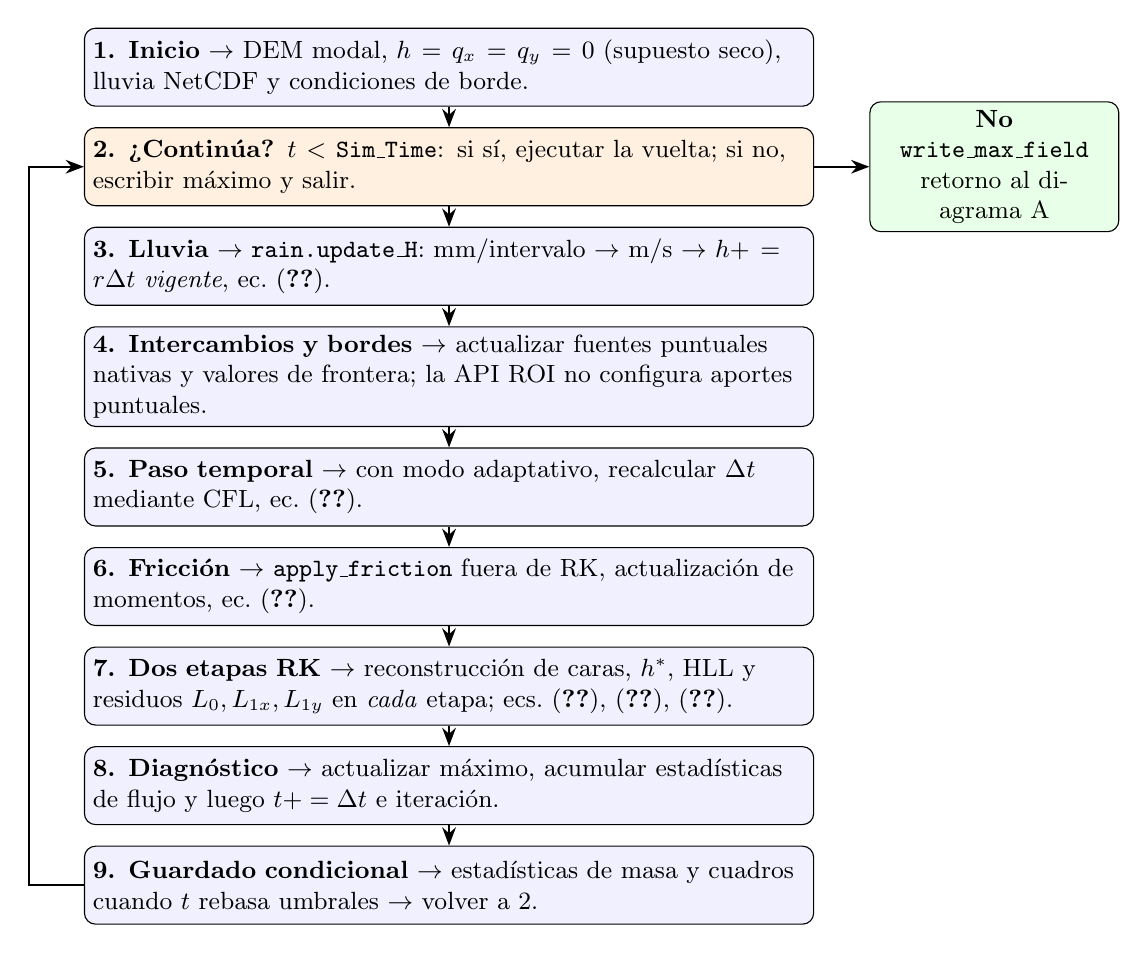
\begin{tikzpicture}[
 node distance=2.6mm,
 paso/.style={draw,rounded corners,fill=blue!6,align=left,text width=9.05cm,
              minimum height=.99cm,inner sep=3pt,font=\small},
 decision/.style={paso,fill=orange!12},
 final/.style={draw,rounded corners,fill=green!9,align=center,text width=2.95cm,
               inner sep=3pt,font=\small},
 flecha/.style={-{Stealth},thick}]
\node[paso] (b1) {\textbf{1. Inicio} $\to$ DEM modal, $h=q_x=q_y=0$ (supuesto seco), lluvia NetCDF y condiciones de borde.};
\node[decision,below=of b1] (b2) {\textbf{2. ¿Continúa?} $t<\texttt{Sim\_Time}$: si sí, ejecutar la vuelta; si no, escribir máximo y salir.};
\node[paso,below=of b2] (b3) {\textbf{3. Lluvia} $\to$ \texttt{rain.update\_H}: mm/intervalo $\to$ m/s $\to$ $h{+}=r\Delta t$ \emph{vigente}, ec.~\eqref{eq:ncrain}.};
\node[paso,below=of b3] (b4) {\textbf{4. Intercambios y bordes} $\to$ actualizar fuentes puntuales nativas y valores de frontera; la API ROI no configura aportes puntuales.};
\node[paso,below=of b4] (b5) {\textbf{5. Paso temporal} $\to$ con modo adaptativo, recalcular $\Delta t$ mediante CFL, ec.~\eqref{eq:cfl}.};
\node[paso,below=of b5] (b6) {\textbf{6. Fricción} $\to$ \texttt{apply\_friction} fuera de RK, actualización de momentos, ec.~\eqref{eq:fricdisc}.};
\node[paso,below=of b6] (b7) {\textbf{7. Dos etapas RK} $\to$ reconstrucción de caras, $h^*$, HLL y residuos $L_0,L_{1x},L_{1y}$ en \emph{cada} etapa; ecs.~\eqref{eq:weak}, \eqref{eq:hll}, \eqref{eq:rk}.};
\node[paso,below=of b7] (b8) {\textbf{8. Diagnóstico} $\to$ actualizar máximo, acumular estadísticas de flujo y luego $t{+}=\Delta t$ e iteración.};
\node[paso,below=of b8] (b9) {\textbf{9. Guardado condicional} $\to$ estadísticas de masa y cuadros cuando $t$ rebasa umbrales $\to$ volver a 2.};
\foreach \prim/\sig in {b1/b2,b2/b3,b3/b4,b4/b5,b5/b6,b6/b7,b7/b8,b8/b9}
  {\draw[flecha] (\prim.south)--(\sig.north);}
\node[final,right=7mm of b2] (fin) {\textbf{No}\\\texttt{write\_max\_field}\\retorno al diagrama A};
\draw[flecha] (b2.east)--(fin.west);
\draw[flecha] (b9.west)--++(-7mm,0) |- (b2.west);
\end{tikzpicture}
\end{center}
\noindent\textbf{Puntos de auditoría.} \texttt{rain.update\_H} en \src{rain/rain.tpp} antecede a \texttt{Tstep\_from\_cfl}; \texttt{apply\_friction} está fuera de \texttt{rk\_stage1/2}. Cada etapa usa \src{swe/dg2/modifiedvars.cpp} para caras hidroestáticas, \src{swe/hll_include.h} para el flujo y \texttt{L0/L1x/L1y} de \src{swe/dg2.cpp} para las tres amplitudes por campo (véanse también \eqref{eq:basis} y \eqref{eq:mean}). El limitador está disponible, \emph{no activado por defecto}; no hay llamada a infiltración en este bucle. El guardado ocurre tras avanzar $t$ sin forzar pasos para coincidir con \texttt{saveint} o el fin: el ASCII no guarda el tiempo físico de cada cuadro, y la API comunica \texttt{time\_s:null}. Estas etapas no incluyen una validación de precisión hidráulica.
\newpage
\noindent Un \texttt{POST /api/flood-scenarios/roi/start/} autenticado valida en memoria el JSON, polígonos, CRS, cobertura geográfica teórica y límites antes de crear trabajo o iniciar adquisición. Solo acepta siete secciones exactas: \texttt{roi}, \texttt{domain}, \texttt{rainfall}, \texttt{rainfall\_profile}, \texttt{terrain}, \texttt{hydraulics}, \texttt{simulation}. Los archivos y binarios son definidos por el servidor, no por el cliente. El POST devuelve 202 con UUID, \texttt{status\_url} y \texttt{results\_url}; el worker fuera del request gestiona adquisición y ejecución. No se afirma cola Celery ni cuota automática de CPU. El estado se conserva en un directorio privado por UUID/propietario con escritura atómica de \texttt{state.json}; cache NASADEM por trabajo y hashes de entradas, ejecutable y utilidad, parámetro, lluvia y COG. Los grupos de proceso de preparación y el solver tienen plazos separados. Un subproceso no constituye por sí solo un sandbox de seguridad.

\begin{center}
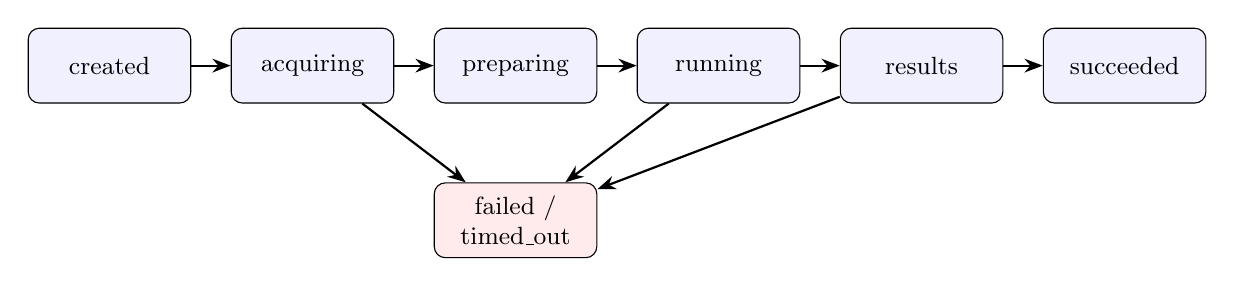
\begin{tikzpicture}[node distance=5mm and 5mm,box/.style={draw,rounded corners,fill=blue!6,align=center,text width=1.83cm,minimum height=.95cm,font=\small},bad/.style={box,fill=red!8},arr/.style={-{Stealth},thick}]
\node[box] (a) {created};\node[box,right=of a] (b) {acquiring};\node[box,right=of b] (c) {preparing};\node[box,right=of c] (d) {running};\node[box,right=of d] (e) {results};\node[box,right=of e] (f) {succeeded};
\foreach \u/\v in {a/b,b/c,c/d,d/e,e/f}{\draw[arr] (\u)--(\v);}
\node[bad,below=1cm of c] (g) {failed / timed\_out};
\draw[arr] (b)--(g);\draw[arr] (d)--(g);\draw[arr] (e)--(g);
\end{tikzpicture}
\end{center}
\noindent\texttt{GET /api/flood-roi-runs/<uuid>/} expone estado; fallos devuelven códigos seguros sin traceback ni rutas internas. \texttt{GET .../results/} responde 409 hasta éxito; en éxito incluye geometría de malla y CRS, unidades \texttt{m above local bed}, cuadros ordenados, estadísticas, máximo, advertencias y metadatos de artefactos. \texttt{GET .../artifacts/<nombre>/} solo sirve TIFF listado de trabajo exitoso al propietario y comprueba SHA256; respuesta completa con \texttt{ETag}, \emph{sin HTTP Range}. Acceso ajeno o nombre no autorizado produce 404. No se expone el ASCII original por esa API. Véanse \src{backend/analyses/roi_flood_runs.py} y \src{docs/api-simulacion-roi.md}.

\subsection{Solicitud completa de ejemplo, no caso calibrado}
{\small\begin{verbatim}
{
 "roi":{"type":"Polygon","coordinates":[[[-92.9998,16.8],[-92.9995,16.8],
 [-92.9995,16.8003],[-92.9998,16.8003],[-92.9998,16.8]]]},
 "domain":{"type":"Polygon","coordinates":[[[-92.9999,16.7998],
 [-92.9993,16.7998],[-92.9993,16.8005],[-92.9999,16.8005],
 [-92.9999,16.7998]]]},
 "rainfall":{"amount":2,"unit":"mm","duration":1,"duration_unit":"s"},
 "rainfall_profile":{"interval_count":2,"seed":7,
                     "distribution":"uniform_balanced"},
 "terrain":{"target_crs":"EPSG:32615","resolution_m":20,
            "resampling":"nearest"},
 "hydraulics":{"manning":0.02,"initial_condition":"dry_zero_velocity",
               "boundary":"free","infiltration":"unsupported",
               "domain_nonurban":true},
 "simulation":{"duration_s":2,"save_interval_s":1,"initial_tstep_s":0.1}
}
\end{verbatim}}
Todos los números de este ejemplo ilustran un contrato, no constituyen tormenta probable, rugosidad recomendada, precisión de 20\,m ni recomendación de duración. La lluvia del ejemplo cae durante 1\,s y la simulación dura 2\,s: la cola restante es seca. La tasa media nominal sería $0.002$\,m/s ($7200$\,mm/h), matemáticamente coherente con 2\,mm en 1\,s pero físicamente extrema; por eso \emph{no} puede presentarse como evento representativo. La selección de dominio y supuestos exige intervención experta.

\noindent\begin{tabularx}{\linewidth}{p{.23\linewidth}X}
\toprule Respuesta & Interpretación correcta\\\midrule
\texttt{202 id/state/urls} & Identifica trabajo admitido; no indica simulación terminada ni validada.\\
\src{frames[i].frame_index} & Orden para reproducir cuadros. \texttt{time\_s:null} significa tiempo físico de ese ASCII no registrado. \texttt{scheduled\_time\_s=i*save\_interval\_s} es tiempo solicitado, no medido.\\
\texttt{maximum} & Máximo de profundidad provisto por el motor; no corresponde a una hora de llegada ni necesariamente a un único cuadro.\\
\texttt{grid/nodata} & CRS métrico y centinela del raster; nodata es desconocido, no profundidad cero.\\
\texttt{artifacts} & TIFF COG numérico con SHA256 y límites geográficos para encuadre, no imagen coloreada Web Mercator ni URL de teselas XYZ.\\
\src{synthetic:true}, \src{hydraulic_accuracy_validated:false} & Identifican carácter hipotético y ausencia de certificación física; no se suprimen en éxito.\\\bottomrule
\end{tabularx}

El motor comprueba guardado \emph{después} de actualizar $t$ y no trunca los pasos al próximo \texttt{saveint} ni al \texttt{sim\_time}. Por eso el adaptador \src{pipeline/hydrology/results.py} ordena índices y calcula solo horas \emph{programadas}; nunca presenta \texttt{scheduled\_time\_s} como observación física exacta. Los ASCII \texttt{.wd} y \texttt{.max} se validan por encabezado, forma, finitud, no negatividad fuera de nodata y malla común; después se exportan a COG \texttt{float32} en CRS proyectado, con hashes origen/destino. La estadística \texttt{wet\_cells} cuenta valores válidos $>0$, \emph{no} una extensión oficial con umbral hidrológico validado. Para MapLibre hay que decodificar/reproyectar a Web Mercator o montar teselas autenticadas por separado: entregar coordenadas EPSG:4326 de encuadre no convierte los píxeles UTM ni agrega soporte Range. No existe API de velocidad ni tiempo de llegada.

\section{Parámetros de servicio, trazabilidad y errores}
\label{sec:operacion}
El archivo \texttt{roi.par} generado declara \texttt{dg2}, \src{DEMfile} \src{terrain.dem}, \texttt{sim\_time}, \texttt{saveint}, \src{initial_tstep}, \src{fpfric} y \src{dynamicrainfile} \src{rain.nc}; para \texttt{free} añade \texttt{bcifile}. La malla de datos y lluvia, la utilidad DEM y el ejecutable se comprueban frente a rutas y hashes de configuración. SHA256 de binario \src{777d50f8d6a926260baa31b4c8ca3ecc0b3ae710494bebb2d4699ccf8c39775c}; de \texttt{generateDG2DEM} \src{ada476fc141d536d09abd4aa1238d192bbddfd627574886ada12784ba0e964a8}. Los hashes identifican bytes usados, no prueban exactitud física ni una licencia de redistribución. Release fuente LISFLOOD-FP 8.0, ejecutable local identificado como 8.0.3 float CPU; instantánea de repositorio al solicitar este documento: \src{615d0ce23eee51df7c130c93a1306958b2d0f0c6}. El \texttt{CODE\_VERSION} configurable identifica la versión declarada del adaptador y debe mantenerse actualizado por operación: su valor por defecto no es garantía de correspondencia automática con HEAD.

\noindent\begin{tabularx}{\linewidth}{p{.28\linewidth}p{.15\linewidth}X}
\toprule Ajuste inicial del servidor & Valor & Significado y restricción\\\midrule
\texttt{FLOOD\_ROI\_DG2\_ENABLED} & true & \texttt{false} desactiva \texttt{start/}; no acredita acceso Earthdata.\\
\texttt{MAX\_CELLS / MAX\_RAIN\_VALUES} & 1000 / 5000 & Presupuestos de malla y valores, no resolución física requerida ni tolerancia hidráulica.\\
\texttt{MAX\_FRAMES / MAX\_TILES} & 5 / 2 & Presupuestos de salidas y teselas; el área contribuyente puede necesitar más.\\
\texttt{TIMEOUT\_S / PREPARATION\_TIMEOUT\_S} & 15 / 120\,s & Plazos del solver y de la fase preparatoria, no duración simulada.\\\bottomrule
\end{tabularx}
El comando \texttt{PYTHONPATH=. python backend/manage.py check\_flood\_service} verifica preparación local sin red; \texttt{--earthdata}, solo con autorización del operador, comprueba una adquisición distinta. No son tests de física. La lectura de credenciales ocurre en entorno privado, nunca en JSON ni en los artefactos públicos. Una solicitud mal formada o fuera de presupuesto es rechazada antes de crear trabajo (400); servicio no disponible o configuración inválida (503); no autenticado (401/403); recurso ajeno o desconocido (404); resultados aún no listos (409). La fase de adquisición puede fallar por credenciales/cobertura; preparación puede fallar por nodata, formato o plazo; el solver por timeout/salida no válida. Los códigos expuestos son sanitizados y no transmiten excepciones ni rutas privadas. \src{backend/config/flood_service.py}, \src{pipeline/hydrology/roi_runner.py}, \src{backend/analyses/roi_flood_runs.py} son la correspondencia operativa.

\section{Evidencia observada y lo que no demuestra}
\label{sec:evidencia}
Se conservan \emph{dos evidencias distintas}, que no deben fusionarse en un resultado regional real:
\begin{enumerate}
\item La unión de adaptador y motor real con proveedor \emph{HGT sintético} terminó en \texttt{succeeded}, malla $9\times8$ a 20\,m, tres cuadros WD y un máximo, cuatro COG EPSG:32615. Registro: \src{data/test-runs/roi-dg2-136934da-7370-4113-b337-36ebc0bcafcc/6c5b38f4-9d14-4c71-912b-04ed7629d94a/state.json}. Prueba continuidad técnica de esa ejecución concreta, no exactitud ni disponibilidad Earthdata para el mismo run.
\item La adquisición \emph{real Earthdata}, separada, guardó comprobante de tesela NASADEM \texttt{n16w094}, ZIP de 14\,251\,621 bytes: \src{data/service-checks/7507c3c0-8ba1-43b1-920e-a35fa58ea70f/proof.json}. Prueba descarga de esa tesela en esa comprobación, no un escenario DG2 ejecutado sobre ella ni autenticidad criptográfica independiente del servidor remoto.
\end{enumerate}
\begin{tabularx}{\linewidth}{p{.23\linewidth}p{.37\linewidth}X}
\toprule Nivel & Evidencia disponible & Comprobación todavía necesaria\\\midrule
Formato e integración & Manifiestos y hashes, NetCDF nativo, ASCII/COG de seam sintético. & Repetir por caso y comparar entradas/salidas; no extrapolar a dominio grande.\\
Matemática numérica & Código de operadores y dimensionalidad descritos aquí. & Ensayos lago en reposo, lecho variable, mojado/seco, convergencia de malla y tiempo.\\
Balance volumétrico & Registro de lluvia y archivo nativo \texttt{.mass}. & Investigar \texttt{Qerror/Verror}, extraer flujos, contrastar $V_f-V_i$ con aportes y fronteras con tolerancia justificada antes de afirmar conservación.\\
Fidelidad física & Ningún evento regional validado en estas evidencias. & DEM/cauces/batimetría, lluvia y niveles independientes, Manning, infiltración, sensibilidad y contraste espacio-temporal externo.\\\bottomrule
\end{tabularx}
Como control, para cada paso ideal $V_{n+1}-V_n\stackrel{?}{=}\Delta t\sum_Kr_K\Delta A-\Delta t\sum_{f\subset\partial\Omega}\widehat q_f\ell_f$ (m$^3$), con convención de normal saliente y tiempo realmente empleado. No usar esta igualdad como resultado observado: hay que determinar cómo el motor integra y registra los aportes y sobrepasos temporales. \texttt{getfattr} registró una advertencia del smoke pendiente de investigación; no se ocultó. Los resultados siguen marcados \texttt{hydraulic\_accuracy\_validated:false}. Un mapa raster que visualmente parece inundación no mide precisión, recall, área verdadera ni error de profundidad. Las escenas NISAR pueden servir de contraste de extensión con hora y máscaras verificadas; una diferencia de retrodispersión no demuestra agua, profundidad o causalidad por sí sola. Sin referencia independiente, el escenario es exploratorio.

\section{Mapa de ecuaciones a código y puntos de auditoría}
\label{sec:mapa}
En la tabla, las rutas nativas se entienden bajo \src{data/tools/lisflood-fp-8.0/runtime/source/}; los nombres de función son anclas auditables más robustas que números de línea cuando cambie el release.
\begin{longtable}{p{.19\linewidth}p{.34\linewidth}p{.38\linewidth}}
\toprule Relación y unidad & Función y salida & Control de interpretación\\\midrule\endhead
\eqref{eq:conserv}--\eqref{eq:flux}, m/s y m$^2$/s$^2$ & \src{swe/flux.cpp}: \texttt{physical\_flux\_x/y}; \src{swe/dg2.cpp}: \texttt{L0/L1x/L1y} & No confundir residuo modal con solo una media; derivadas dividen por metros.\\
\eqref{eq:vertices}, m & \src{preprocess/generateDG2DEM.cpp} y \src{swe/dg2/fields.cpp}: tres \texttt{.dem*} & Comparar cotas y centinela; los coeficientes no son pendientes GIS en m/m.\\
$z^*,h^*,q^*$, m, m, m$^2$/s & \src{swe/dg2/modifiedvars.cpp}: \texttt{initialise\_Zstar}, \texttt{update\_Hstar}, \texttt{discharge\_star} & Cara seca no implica prueba de positividad global.\\
\eqref{eq:hll}, m$^2$/s y m$^3$/s$^2$ & \src{swe/hll_include.h}: rama intermedia; \src{swe/dg2.cpp}: \texttt{update\_fluxes} & Componente transversal usa contacto elegido, no HLL vectorial directo.\\
\eqref{eq:fricdisc}, m$^2$/s & \src{swe/dg2/friction.cpp}: \texttt{friction}, \texttt{apply\_friction} & Separar pendiente adimensional y fuerza de momento; operador fuera RK.\\
\eqref{eq:cfl}, s; \eqref{eq:rk}, unidades de $U$ & \src{swe/dg2.cpp}: \texttt{min\_dt}, \texttt{rk\_stage1/2}, \texttt{solve} & Paso CFL condicional a modo adaptativo; no sincroniza exactamente cuadros.\\
\eqref{eq:rainbal}--\eqref{eq:ncrain}, m y m/s & \src{pipeline/hydrology/rainfall.py}, \src{pipeline/hydrology/rainfall_netcdf.py}, \src{rain/rain.tpp} & Diferenciar acumulado mm, horas de archivo y m/s del motor; revisar orden previo al CFL.\\
Profundidad $h$, m sobre lecho & \src{pipeline/hydrology/results.py}: \texttt{summarize\_results}, \texttt{export\_depth\_cog} & Nodata desconocido; tiempo real ausente; COG numérico en CRS métrico.\\\bottomrule
\end{longtable}

\section{Límites de interpretación y tareas para un caso científico}
\label{sec:limites}
Antes de interpretar una simulación real deben fijarse evento, dominio contribuyente, origen temporal UTC, calidad y resolución del DEM, datum de niveles, batimetría/cauces, flujo inicial, condición observada de borde, lluvia representativa, infiltración (no soportada en esta ruta), Manning espacial o justificación de valor uniforme y relación con zonas urbanas omitidas. Una frontera FREE no resuelve automáticamente estas preguntas. Establecer umbral de extensión y máscaras de nodata y agua permanente; comparar una observación al tiempo que efectivamente representa el cuadro, no el máximo temporal frente a una instantánea. Mientras el ASCII no registre tiempo físico, esa comparación puntual debe declarar su incertidumbre temporal o no realizarse. Elegir y registrar tolerancias de balance y convergencia \emph{antes} de usar resultados; no inventar porcentajes de error aceptables. Comparar con datos independientes separados de cualquier ajuste. El coste de una malla mayor se debe medir: los límites iniciales de servidor son presupuestos operativos pequeños, no capacidad regional verificada.

\section{Cómo leer y usar los resultados de una simulación}
\label{sec:leer-resultados}

Esta sección aterriza la parte anterior en una pregunta práctica: tengo un resultado descargado, ¿qué puedo
decir de él y qué no? Cada subsección corresponde a un campo de la respuesta de la API.

\subsection{Profundidad $h$: «m sobre el lecho local»}

Los valores de profundidad están en metros \emph{sobre el lecho}, no en altitud absoluta. Dos consecuencias:
\begin{itemize}
  \item Una profundidad de $0.30$\,m significa 30\,cm de agua sobre el terreno en esa celda, medidos a partir de
        la cota del DEM en la celda. No es la cota de la superficie del agua.
  \item Para comparar con una referencia externa (por ejemplo, el nivel de un río medido), hay que cuidar que
        ambos estén en el mismo datum vertical. NASADEM trae alturas referidas al geoide EGM96; los niveles de
        una estación pueden estar en otro datum.
\end{itemize}

\subsection{Cuadros y máximo}

\begin{description}[style=nextline]
  \item[Cuadros.] Cada cuadro es un instante guardado del campo de profundidad. El orden (\texttt{frame\_index}) es
        fiable; el tiempo físico de cada uno \emph{no está registrado} en el ASCII del motor, y por eso la API
        devuelve \texttt{time\_s:null}. El tiempo \texttt{scheduled\_time\_s} es el solicitado, no el medido,
        porque el motor no trunca los pasos para coincidir con \texttt{saveint}.
  \item[Máximo.] El máximo temporal en cada celda a lo largo de toda la simulación. No es un instante; es el
        envolvente. No indica cuándo llegó el agua ni tiene una única hora asociada.
\end{description}

\begin{cuidado}
Comparar el \emph{máximo temporal} de la simulación con una \emph{instantánea} de satélite es comparar cosas
distintas. Una observación de una sola hora solo puede contrastarse con el cuadro que represente esa hora, y
mientras el ASCII no registre tiempo físico, esa comparación debe declarar su incertidumbre temporal o no
hacerse.
\end{cuidado}

\subsection{NoData y celdas mojadas}

El valor \texttt{nodata} marca celdas sin dato; es \emph{desconocido}, no «profundidad cero». La estadística
\texttt{wet\_cells} cuenta valores válidos mayores que cero. No usa ningún umbral hidrológico: una celda con
$10^{-6}$\,m cuenta como mojada, y por eso no debe leerse como «área inundada» sin definir antes un umbral
físicamente motivado.

\subsection{El COG y su uso en un mapa}

El archivo entregado es un GeoTIFF optimizado para la nube (COG) en el CRS métrico elegido, con los valores
numéricos de profundidad. No es una imagen coloreada ni un conjunto de teselas. Para mostrarlo en un visor web
en proyección Web Mercator hay que decodificar y reproyectar, o montar teselas autenticadas aparte. El
servicio responde con el archivo completo y \texttt{ETag}, sin soporte HTTP Range.

\subsection{Los distintivos que acompañan todo resultado}

Dos campos acompañan siempre a un resultado exitoso: \texttt{synthetic:true} y
\texttt{hydraulic\_accuracy\_validated:false}. No se suprimen, aunque la simulación termine sin errores. Son el
recordatorio de que el resultado pertenece al nivel de \emph{escenario} (sección~\ref{sec:tres-niveles}).

\subsection{Qué haría falta para pasar de «técnicamente correcto» a «científicamente defendible»}

La tabla~\ref{tab:de-tecnico-a-cientifico} traduce la sección~\ref{sec:evidencia} en tareas.

\begin{table}[htbp]
\centering\small
\begin{tabularx}{\linewidth}{p{.27\linewidth}X}
\toprule
\textbf{Tarea} & \textbf{Por qué es necesaria}\\\midrule
Definir el dominio contribuyente & La ROI de consulta no es la cuenca que alimenta el flujo.\\
Fijar condiciones de borde justificadas & Una frontera \texttt{free} o cerrada puede dominar el resultado.\\
Elegir Manning y justificarlo & La fricción controla velocidades y tiempos de llegada.\\
Incorporar infiltración & La ruta actual no la aplica: toda la lluvia se queda en superficie.\\
Comprobar el balance volumétrico & Verificar que el volumen final iguale aportes menos salidas, con tolerancia declarada \emph{antes}.\\
Hacer ensayos numéricos clásicos & Lago en reposo, lecho variable, mojado/seco, convergencia de malla y de paso de tiempo.\\
Contrastar con datos independientes & Sin referencia externa, el resultado es exploratorio.\\\bottomrule
\end{tabularx}
\caption{De un resultado técnicamente correcto a uno científicamente defendible.}
\label{tab:de-tecnico-a-cientifico}
\end{table}

\begin{intuicion}
Una simulación sin validar \emph{sí} tiene valor: sirve para explorar escenarios, para entender qué parte del
relieve concentra el agua y para detectar errores de configuración. Lo que no puede hacer es sustituir una
medición ni una predicción verificada. Mantener esa frontera es lo que permite usar el simulador sin engañar
a quien lea sus mapas.
\end{intuicion}


\section{Cómo verificar un simulador de inundación}
\label{sec:verificacion}

Un simulador numérico produce siempre una respuesta, correcta o no. Que el mapa se vea plausible no demuestra
nada: un esquema con un error de signo en un término fuente puede generar láminas de agua de aspecto
perfectamente razonable. Por eso la práctica habitual es \emph{verificar} (¿resuelve el código las ecuaciones
que dice resolver?) antes de \emph{validar} (¿describen esas ecuaciones la realidad?). Esta sección explica la
verificación; la validación contra observaciones de un evento real es una tarea distinta y está fuera del
alcance actual del simulador (sección~\ref{sec:limites}).

\begin{atencion}
Verificar no es validar. Un código verificado resuelve bien un modelo; el modelo puede seguir siendo una mala
descripción del terreno concreto, de la lluvia real o de la fricción real. Ninguna de las pruebas de esta
sección convierte el resultado en una predicción.
\end{atencion}

\subsection{Prueba 1: el lago en reposo}

\paragraph{Planteamiento.} Se toma un terreno cualquiera, con relieve irregular, y se llena parcialmente de
agua con superficie libre horizontal $\eta=h+z_b=\text{constante}$ y velocidad cero. Sin lluvia, sin fricción
activa y sin entradas, la solución exacta es que \emph{nada se mueve}.

\paragraph{Qué comprueba.} Es la prueba de la propiedad «bien equilibrado» (\emph{well-balanced}). En las
ecuaciones, el gradiente de presión $\tfrac12 g\,\partial_x(h^2)$ debe cancelarse exactamente con el término de
pendiente del lecho $-gh\,\partial_xz_b$. Si la discretización de ambos términos no es coherente, el esquema
inventa corrientes espurias sobre un fondo irregular. La reconstrucción hidrostática (sección~\ref{sec:dg2})
existe precisamente para garantizar esa cancelación.

\paragraph{Criterio de éxito.} La máxima velocidad espuria tras muchos pasos de tiempo debe ser del orden del
error de redondeo ($\lesssim10^{-10}$\,m/s en doble precisión), no del orden de $10^{-2}$\,m/s.

\begin{ejemplo}[Cuánto es «cero»]
Si tras 10\,000 pasos la velocidad máxima es $3\times10^{-13}$\,m/s, la prueba pasa. Si es $4\times10^{-3}$\,m/s,
el esquema no está equilibrado: esa velocidad, mantenida un día, movería agua $\approx350$\,m, y un modelo con
ese defecto «inundaría» sin lluvia.
\end{ejemplo}

\subsection{Prueba 2: la rotura de presa de Ritter}

La solución analítica de la ecuación~\eqref{eq:ritter} (sección~\ref{sec:der-swe}) permite medir el error del
simulador sobre una onda real, con un frente que avanza sobre fondo seco. Es una prueba exigente porque
combina tres dificultades: una discontinuidad inicial, un borde húmedo--seco y un perfil parabólico suave en
el abanico.

\paragraph{Procedimiento.}
\begin{enumerate}
  \item Se inicializa $h=h_0$ en $x<0$ y $h=0$ en $x>0$, con fondo plano, $n_M=0$ y sin lluvia.
  \item Se avanza hasta un tiempo $T$ (por ejemplo 6\,s) y se extrae $h(x,T)$ del simulador.
  \item Se compara con la ecuación~\eqref{eq:ritter} en los centros de celda, calculando un error global
        \[
          E=\frac{1}{N}\sum_{i=1}^{N}\bigl|h_i^{\text{num}}-h(x_i,T)\bigr| .
        \]
  \item Se repite con la malla refinada y se estudia cómo baja $E$ (prueba 4).
\end{enumerate}

\paragraph{Qué esperar.} El frente numérico está ligeramente suavizado: un esquema de segundo orden reparte la
discontinuidad en pocas celdas. El error se concentra ahí y en el borde húmedo--seco. Lo que \emph{no} debe
ocurrir es que el frente adelante o retrase de forma sistemática más de unas celdas con respecto a
$x_f=2c_0T$ (con $c_0=\sqrt{gh_0}$), ni que aparezcan profundidades negativas.

\subsection{Prueba 3: balance de masa}

El simulador resuelve una ley de conservación, así que el volumen de agua debe cambiar solo por lo que entra
y sale. Con $V^n=\sum_K h_K^n\,A_K$ y sumando todas las celdas,
\begin{equation}
  V^{n+1}-V^{n}=\Delta t\,\Bigl(\underbrace{\sum_K r_K A_K}_{\text{lluvia}}
  -\underbrace{\sum_{\text{fronteras}}\textstyle\int q_n\,\dd\ell}_{\text{salida neta}}\Bigr).
  \label{eq:balance}
\end{equation}
Las contribuciones de las caras interiores se cancelan por pares, porque el flujo numérico que sale de una
celda es exactamente el que entra a su vecina; solo sobreviven las fronteras. Esta cancelación es una
propiedad del esquema conservativo: si se rompe, hay un defecto en el código.

\begin{ejemplo}[Un balance de lluvia]
Un dominio de $4\ \mathrm{km}^2$ con frontera cerrada recibe $60$\,mm de lluvia. El volumen añadido debe ser
$60\times10^{-3}\ \mathrm{m}\times4\times10^{6}\ \mathrm{m}^2=2.4\times10^{5}\ \mathrm{m}^3$. En una celda de
$20\times20$\,m ($400\ \mathrm{m}^2$) corresponde a $24\ \mathrm{m}^3$. Si el simulador reporta un volumen
final que difiere en más de un error de redondeo, el balance no cierra.
\end{ejemplo}

Existe una excepción legítima: el recorte de profundidades negativas minúsculas (limpieza húmedo--seco) puede
introducir un residuo de masa muy pequeño. Un buen informe lo \emph{cuantifica} en lugar de ocultarlo.

\subsection{Prueba 4: orden de convergencia}

Si el esquema es de orden $p$, el error cae como $E\propto\Delta x^{p}$. Con dos mallas, $\Delta x_1>\Delta x_2$ y
errores $E_1$ y $E_2$, el orden observado es
\begin{equation}
  p_{\text{obs}}=\frac{\ln(E_1/E_2)}{\ln(\Delta x_1/\Delta x_2)} .
  \label{eq:orden}
\end{equation}

\begin{ejemplo}[Un orden observado hipotético]
Supóngase $E_1=0.040$\,m con $\Delta x_1=10$\,m y $E_2=0.011$\,m con $\Delta x_2=5$\,m. Entonces
$p_{\text{obs}}=\ln(0.040/0.011)/\ln2=\ln(3.64)/0.693=1.86$.
Un valor cercano a 2 es el esperable para un esquema de segundo orden en zonas suaves. Los números de este
ejemplo son ilustrativos: no son resultados medidos del simulador.
\end{ejemplo}

\begin{cuidado}
Con soluciones discontinuas el orden observado cae hacia 1, porque el error está dominado por la
discontinuidad. Una prueba con solución suave (una onda larga de baja amplitud) mide el orden formal; la
rotura de presa mide la robustez. Ambas son útiles, pero no se interpretan igual.
\end{cuidado}

\subsection{Prueba 5: sensibilidad a los parámetros}

Cuando no hay solución exacta, se estudia cómo cambia el resultado al variar una entrada. La tabla
siguiente resume qué se espera cualitativamente; sirve para detectar comportamientos que contradicen la física.

\begin{table}[htbp]
\centering
\caption{Sensibilidades cualitativas esperadas del simulador.}
\label{tab:sensibilidad}
\small
\begin{tabularx}{\linewidth}{@{}lXX@{}}
\toprule
Cambio de entrada & Efecto esperado & Señal de alarma \\
\midrule
Duplicar la lluvia & Más volumen y mayor profundidad máxima, aunque no lineal & Profundidad que disminuye \\
Aumentar $n_M$ & Flujo más lento; picos retrasados y más altos localmente & Velocidades mayores \\
Refinar la malla & Frente más nítido; resultado global estable & Cambio global de volumen \\
Reducir el paso (CFL menor) & Resultado casi idéntico & Cambio grande de la solución \\
Terreno más suave & Menos encharcamiento local & Más encharcamiento \\
\bottomrule
\end{tabularx}
\end{table}

\subsection{Registro de ensayos}

Para que una verificación sea auditable, cada ensayo se registra con los mismos campos. Una plantilla mínima:

\begin{table}[htbp]
\centering
\caption{Plantilla de registro de una prueba de verificación.}
\label{tab:registro}
\small
\begin{tabularx}{\linewidth}{@{}lX@{}}
\toprule
Campo & Contenido \\
\midrule
Identificador & Nombre corto y fecha de la prueba \\
Versión & Versión del código y del esquema de entrada \\
Malla & $\Delta x$, número de celdas, CRS \\
Parámetros & $n_M$, lluvia, CFL, tiempo final \\
Métrica & Error $E$, velocidad espuria, residuo de masa \\
Criterio & Umbral decidido \emph{antes} de ejecutar \\
Resultado & Valor medido y veredicto (pasa/no pasa) \\
Observaciones & Anomalías, limpiezas húmedo--seco aplicadas \\
\bottomrule
\end{tabularx}
\end{table}

Fijar el criterio \emph{antes} de ejecutar es la parte importante: elegirlo después de ver el número es la forma
más común de que una verificación sea decorativa.


\section{Fuentes y correspondencia de versión}
\begin{enumerate}
\item Shaw, J. y cols. (2021), ``LISFLOOD-FP 8.0: the new discontinuous Galerkin shallow-water solver for multi-core CPUs and GPUs'', \emph{Geoscientific Model Development} 14, 3577--3602. \url{https://doi.org/10.5194/gmd-14-3577-2021}. Fuente de contexto del método publicado, no sustituto del cotejo del ejecutable concreto.
\item LISFLOOD-FP 8.0, artefacto original: \url{https://zenodo.org/records/4073011}; guía de los desarrolladores: \url{https://www.seamlesswave.com/LISFLOOD8.0}. Las ecuaciones atribuidas a \emph{esta ejecución} se cotejan con la fuente nativa local bajo \src{data/tools/lisflood-fp-8.0/runtime/source/}, no se atribuyen a una extracción incompleta de la página HTML del artículo.
\item NASADEM User Guide V1.3, producto HGT y referencia vertical EGM96: \url{https://lpdaac.usgs.gov/documents/2237/NASADEM_User_Guide_V13.pdf}. La referencia no certifica una elevación particular.
\item Contratos actuales: \src{docs/api-simulacion-roi.md}, \src{docs/configuracion-servicio-inundacion.md}, \src{docs/distribucion-lluvia.md}, \src{docs/dem-dg2.md}, \src{docs/resultados-dg2.md} y código citado en el \S\ref{sec:mapa}. Documentos conceptuales anteriores describen propuestas históricas y no desplazan el contrato implementado. La identificación de licencia en Zenodo no autoriza por sí sola redistribución del binario; revisar obligaciones antes de publicarlo.
\end{enumerate}

\clearpage

\part{Radiación solar sobre el terreno}
\label{part:solar}

\section{Alcance de la simulación solar}
\label{sec:solar-alcance}

Esta parte describe exclusivamente el comportamiento implementado en \src{pipeline/solar/*.py} y
\src{backend/solar/*.py}. La cadena sigue este orden:
\begin{enumerate}
  \item resuelve el tiempo y la atmósfera;
  \item prepara un DEM NASADEM HGT en una grilla métrica;
  \item calcula la posición solar con NREL SPA;
  \item estima la irradiancia normal directa (DNI) de cielo despejado con pvlib Ineichen;
  \item deriva las normales topográficas;
  \item proyecta la DNI sobre el terreno.
\end{enumerate}
El resultado es un modelo climatológico instantáneo de irradiancia directa incidente, en
W\,m$^{-2}$, no una medición meteorológica ni una predicción validada localmente. Los píxeles inválidos se
conservan como NoData.

\noindent\textbf{Lo que no se calcula.} No se calcula absorción por materiales, reflexión, transmisión,
radiación difusa ni sombra topográfica.

% PENDIENTE: aquí irán las ecuaciones detalladas de la cadena solar (posición solar, DNI, normales,
% proyección sobre el terreno) cuando se incorpore el documento técnico de pipeline/solar.

\section{Fundamentos conceptuales de la irradiancia solar sobre el terreno}
\label{sec:solar-fundamentos}

\begin{atencion}
Esta sección y las siguientes explican la \emph{física general} en la que se basa la cadena solar. Son material
de apoyo para entender las ideas, no una descripción línea por línea del código. El comportamiento
implementado es exactamente el de la sección~\ref{sec:solar-alcance}; las fórmulas de abajo son las formas
estándar de la literatura, y las constantes y ajustes de cada biblioteca (NREL SPA, pvlib) deben consultarse
en su documentación.
\end{atencion}

\subsection{Cuatro preguntas, cuatro etapas}

El simulador solar responde, en este orden, cuatro preguntas independientes:
\begin{enumerate}
  \item \textbf{¿Dónde está el Sol en este instante?} Es astronomía: una función del lugar y del tiempo.
  \item \textbf{¿Cuánta energía del Sol llega a la superficie con cielo despejado?} Es atmósfera: la irradiancia
        normal directa (DNI).
  \item \textbf{¿Cómo está inclinado el terreno en cada píxel?} Es geometría del relieve: la normal a la
        superficie.
  \item \textbf{¿Cuánta de esa energía incide realmente sobre esa superficie inclinada?} Es el producto de las
        tres anteriores.
\end{enumerate}

\begin{figure}[htbp]
\centering
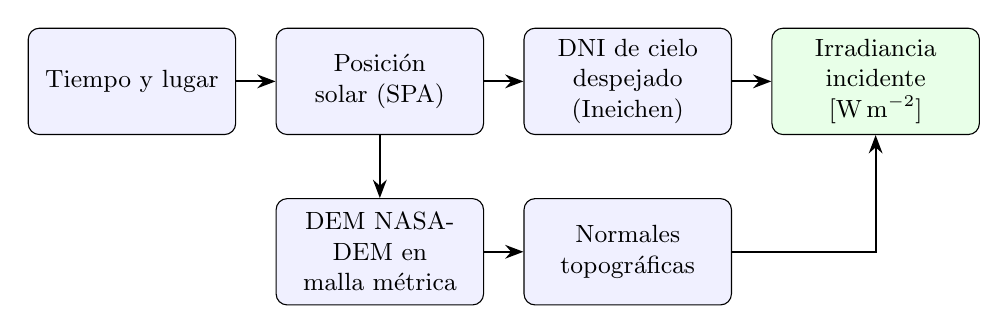
\begin{tikzpicture}[node distance=5mm,
  caja/.style={draw,rounded corners,fill=blue!6,align=center,text width=2.4cm,minimum height=1.35cm,font=\small},
  sal/.style={caja,fill=green!9},
  fl/.style={-{Stealth},thick}]
\node[caja] (a) {Tiempo y lugar};
\node[caja,right=of a] (b) {Posición solar (SPA)};
\node[caja,right=of b] (c) {DNI de cielo despejado (Ineichen)};
\node[caja,below=8mm of b] (d) {DEM NASADEM en malla métrica};
\node[caja,right=of d] (e) {Normales topográficas};
\node[sal,right=of c] (f) {Irradiancia incidente [W\,m$^{-2}$]};
\draw[fl] (a)--(b); \draw[fl] (b)--(c); \draw[fl] (c)--(f);
\draw[fl] (d)--(e); \draw[fl] (e.east) -| (f.south);
\draw[fl] (b.south) -- (d.north);
\end{tikzpicture}
\caption{Las etapas conceptuales de la cadena solar y cómo se combinan. La proyección final combina la
dirección del Sol, la DNI y la normal del terreno.}
\label{fig:cadena-solar}
\end{figure}

\subsection{Posición del Sol}

La posición del Sol se describe con dos ángulos: el \textbf{cenit} $\theta_z$ (ángulo con la vertical local;
0$^\circ$ es el Sol justo encima) y el \textbf{azimut} $\phi_s$ (dirección horizontal, medida aquí desde el norte
hacia el este). La \textbf{elevación} es el complemento del cenit, $90^\circ-\theta_z$. En una aproximación
sencilla, el coseno del cenit solo depende de la latitud $\varphi$, la declinación solar $\delta$ (la latitud
sobre la que el Sol está en el cenit ese día) y el ángulo horario $\omega$ (cuánto ha girado la Tierra desde el
mediodía solar):
\begin{equation}
  \cos\theta_z=\sin\varphi\sin\delta+\cos\varphi\cos\delta\cos\omega .
  \label{eq:cenit}
\end{equation}
Los algoritmos de alta exactitud, como el NREL SPA (\emph{Solar Position Algorithm}), incluyen además la
excentricidad de la órbita terrestre, la nutación, la refracción atmosférica y la corrección de tiempo
(ecuación del tiempo). Su incertidumbre declarada es del orden de milésimas de grado, mucho menor que cualquier
otra fuente de error del problema. Por eso, en esta cadena, la posición solar no es la limitación.

\subsection{Irradiancia normal directa con cielo despejado}

La \textbf{DNI} es la potencia por unidad de área que llega del Sol en línea recta sobre una superficie
perpendicular a los rayos. Fuera de la atmósfera sería la irradiancia extraterrestre $I_0$ (del orden de
$1361$\,W\,m$^{-2}$, con una variación anual pequeña por la distancia Tierra--Sol). Al atravesar la atmósfera,
una parte se absorbe y se dispersa, y lo que queda es la DNI. Una forma funcional habitual para cielo despejado,
del tipo de la de Ineichen y Perez, es
\begin{equation}
  \mathrm{DNI}\approx I_0\,b\,\exp\!\bigl[-0.09\,m\,(T_L-1)\bigr],
  \label{eq:dni}
\end{equation}
donde $m$ es la masa de aire, $T_L$ el \textbf{turbidez de Linke} y $b$ un coeficiente que depende de la altitud.
Las ideas físicas son dos:
\begin{itemize}
  \item La \textbf{masa de aire} $m$ mide cuánta atmósfera atraviesa el rayo. Vale $\approx1$ con el Sol en el cenit
        y crece cuando el Sol baja. Una aproximación estándar (Kasten y Young) da $m\approx2.0$ para
        $\theta_z=60^\circ$ y mucho más cerca del horizonte.
  \item El \textbf{turbidez de Linke} $T_L$ resume la opacidad de la atmósfera por aerosoles y vapor de agua: es
        el número de atmósferas «limpias y secas» que producirían la misma extinción. Valores bajos (2--3)
        son cielos muy limpios; valores altos (5 o más), cielos turbios o húmedos.
\end{itemize}
La forma exponencial es una ley de Beer--Lambert: la energía decae exponencialmente con el camino óptico, que
es proporcional a $m(T_L-1)$.

\figura{sol_dni_aire}{0.66}{Estructura de la DNI de cielo despejado (como fracción de $I_0$, a nivel del mar) en
función del cenit para cuatro valores del turbidez de Linke. Es una ilustración de la forma funcional; la
implementación de pvlib añade ajustes y límites adicionales.}

\begin{cuidado}
Ni la ecuación~\eqref{eq:dni} ni la figura describen el clima real. Representan una atmósfera \emph{climatológica}
y despejada: no incluyen nubes. Una DNI calculada con esta forma funcional es una cota superior razonable de lo
que habría en ese lugar y momento si el cielo estuviera claro, no una predicción de lo que ocurrió.
\end{cuidado}

\subsection{La normal del terreno desde un DEM}

Un DEM da la elevación $z$ en una malla. La pendiente en cada celda se estima con diferencias finitas entre
celdas vecinas, $\partial z/\partial x$ y $\partial z/\partial y$. La normal unitaria a la superficie
$z(x,y)$ es
\begin{equation}
  \hat{\mathbf n}=\frac{\bigl(-\partial_xz,\ -\partial_yz,\ 1\bigr)}{\sqrt{1+(\partial_xz)^2+(\partial_yz)^2}},
  \label{eq:normal}
\end{equation}
con $x$ hacia el este, $y$ hacia el norte y la tercera componente hacia arriba. La \textbf{pendiente}
$\beta$ es el ángulo entre $\hat{\mathbf n}$ y la vertical, $\tan\beta=\sqrt{(\partial_xz)^2+(\partial_yz)^2}$, y la
\textbf{orientación} (\emph{aspect}) es la dirección horizontal hacia la que mira la ladera.

La resolución del DEM importa: las pendientes se calculan sobre celdas vecinas, de modo que la rugosidad
más fina que la malla se pierde. Con celdas de 20\,m, las irregularidades de decenas de centímetros o de
unos pocos metros no existen para el cálculo.

\subsection{Proyectar la DNI sobre la superficie}

Si $\hat{\mathbf s}$ es el vector unitario que apunta hacia el Sol,
$\hat{\mathbf s}=(\cos e\,\sin\phi_s,\ \cos e\,\cos\phi_s,\ \sin e)$ con $e$ la elevación, entonces la irradiancia
directa sobre una superficie con normal $\hat{\mathbf n}$ es
\begin{equation}
  I_{\mathrm{dir}}=\mathrm{DNI}\ \max\!\bigl(0,\ \hat{\mathbf n}\!\cdot\!\hat{\mathbf s}\bigr),
  \qquad
  \hat{\mathbf n}\!\cdot\!\hat{\mathbf s}=\cos\theta_z\cos\beta+\sin\theta_z\sin\beta\cos(\phi_s-\phi_n),
  \label{eq:proyeccion}
\end{equation}
donde $\phi_n$ es la orientación de la ladera. El coseno del ángulo $\theta$ entre la normal y los rayos es lo
que, intuitivamente, mide cuán «de frente» recibe la superficie al Sol (figura~\ref{fig:sol_geometria}).

\figura{sol_geometria}{0.62}{El ángulo $\theta$ entre la normal $\hat n$ y la dirección hacia el Sol $\hat s$
determina la fracción de DNI que incide sobre la superficie, $\cos\theta$. En el ejemplo: pendiente
$\beta=25^\circ$, cenit $40^\circ$ y ladera mirando lejos del Sol, con $\theta=65^\circ$.}

\begin{ejemplo}[Una ladera de $25^\circ$ con el Sol a $40^\circ$ de elevación]
Con $\theta_z=50^\circ$ (elevación $40^\circ$), $\beta=25^\circ$ y $\mathrm{DNI}=800$\,W\,m$^{-2}$ (valor
ilustrativo), el factor geométrico depende de hacia dónde mire la ladera:
\begin{center}\small
\begin{tabular}{lccc}
\toprule
Orientación respecto al Sol & $\hat n\!\cdot\!\hat s$ & Irradiancia directa & Respecto a terreno plano\\\midrule
Terreno plano ($\beta=0$) & $0.643$ & $514$\,W\,m$^{-2}$ & $1.00$\\
Mira hacia el Sol ($\phi_s-\phi_n=0^\circ$) & $0.906$ & $725$\,W\,m$^{-2}$ & $1.41$\\
Lateral ($90^\circ$) & $0.583$ & $466$\,W\,m$^{-2}$ & $0.91$\\
Da la espalda ($180^\circ$) & $0.259$ & $207$\,W\,m$^{-2}$ & $0.40$\\\bottomrule
\end{tabular}
\end{center}
La primera fila es $\cos50^\circ$; la segunda es $\cos(50^\circ-25^\circ)=\cos25^\circ$, porque cuando la ladera
mira al Sol, la normal queda inclinada $25^\circ$ hacia él. Una ladera orientada hacia el Sol puede recibir un
$41\,\mathrm{\%}$ más de DNI que un terreno plano, y la opuesta, un $60\,\mathrm{\%}$ menos.
\end{ejemplo}

\figura{sol_cos_pendiente}{0.66}{Fracción de DNI incidente $\max(0,\cos\theta)$ en función de la pendiente para
un cenit de $50^\circ$ y tres orientaciones. La ladera que mira al Sol gana al aumentar la pendiente hasta que
la normal se alinea con los rayos ($\beta=50^\circ$); la que le da la espalda pierde hasta llegar a cero.}

\subsection{Del ejemplo a un mapa píxel a píxel}

La ecuación~\eqref{eq:proyeccion} se evalúa independientemente en cada celda del DEM. La
figura~\ref{fig:sol_terreno} lo ilustra con un terreno \emph{sintético}: dos colinas, con el Sol al sureste y a
$40^\circ$ de elevación. Las laderas que miran hacia el sureste aparecen más brillantes que el terreno plano
(índice mayor que 1 en la escala de la figura); las que miran al noroeste, más oscuras. Es una imagen
conceptual; no es una salida del pipeline.

\figura{sol_terreno}{1.0}{Terreno sintético (izquierda) y factor geométrico $\max(0,\hat n\!\cdot\!\hat s)$
relativo al de un terreno plano (derecha), con el Sol al sureste (azimut $135^\circ$) y a $40^\circ$ de
elevación. Resolución de 20\,m.}

\subsection{Lo que el modelo no incluye, y qué implica}

La cadena implementada calcula la DNI proyectada sobre el terreno y nada más. En concreto, \emph{no} calcula:
\begin{description}[style=nextline]
  \item[Sombra topográfica proyectada.] Una celda puede estar orientada hacia el Sol y, aun así, estar en
        sombra porque una montaña tapa los rayos. El modelo solo considera la orientación local de la
        superficie. Con el Sol bajo, este efecto puede ser grande y el resultado \emph{sobreestima} la
        irradiancia en los valles.
  \item[Radiación difusa.] La luz dispersada por la atmósfera también llega a la superficie, incluso a la
        sombra. Sumar solo la componente directa subestima la irradiancia total.
  \item[Reflexión del terreno vecino.] Una ladera iluminada puede reflejar luz hacia otra.
  \item[Absorción, reflexión y transmisión por materiales.] La parte de la energía que un material absorbe o
        refleja no se modela; el resultado es la energía \emph{incidente}, no la absorbida.
  \item[Nubes.] La atmósfera es de cielo despejado.
\end{description}
Cada omisión tiene una dirección de sesgo conocida, y eso permite interpretar el resultado con honestidad: es
una cota de la componente directa con cielo despejado.

\subsection{Cómo leer la salida}

La salida es una irradiancia directa incidente, en W\,m$^{-2}$, por píxel. Reglas de lectura:
\begin{itemize}
  \item Es \emph{instantánea}: corresponde al instante elegido, no a una energía diaria (que habría que obtener
        integrando en el tiempo, en W\,h\,m$^{-2}$).
  \item Los píxeles inválidos se conservan como NoData, no como cero. Un cero significaría una celda oscura;
        NoData, que no hay respuesta.
  \item Es un modelo climatológico, no una medición: no se debe comparar con un piranómetro en un día nublado
        y concluir que «el modelo falla».
  \item Para validarlo habría que comparar contra mediciones de DNI en cielo despejado en ese lugar y,
        por separado, evaluar el efecto del relieve.
\end{itemize}

\begin{table}[htbp]
\centering\small
\begin{tabularx}{\linewidth}{p{.28\linewidth}p{.18\linewidth}X}
\toprule
\textbf{Fuente de error} & \textbf{Sesgo} & \textbf{Dónde pesa más}\\\midrule
Sombra topográfica no calculada & Sobreestima & Valles y laderas con el Sol bajo.\\
Radiación difusa omitida & Subestima el total & Zonas sombreadas y cielos turbios.\\
Cielo despejado supuesto & Sobreestima respecto al clima real & Temporada de lluvias, nubosidad frecuente.\\
Resolución del DEM & Suaviza pendientes & Relieve muy accidentado.\\
Turbidez de Linke climatológico & Incertidumbre en la DNI & Lugares con aerosoles variables.\\\bottomrule
\end{tabularx}
\caption{Fuentes de error de la irradiancia directa calculada y su dirección.}
\label{tab:errores-solar}
\end{table}


\section{Un día completo sobre el terreno: ejemplo ilustrativo}
\label{sec:solar-dia}

\begin{atencion}
Esta sección es un ejemplo \emph{conceptual} con fórmulas estándar de cielo despejado. No describe la salida del
simulador del proyecto, no incluye sombras, nubes ni radiación difusa, y las cifras no están validadas contra
medidas. Sirve para entender de dónde salen los órdenes de magnitud.
\end{atencion}

\subsection{Declinación y duración del día}

Se toma el 15 de noviembre (día 319 del año) en una latitud de $16.8^\circ$\,N, representativa del sur de
México. La aproximación de Cooper da una declinación
$\delta\approx23.45^\circ\sin[360^\circ(284+319)/365]=-19.1^\circ$.
El ángulo horario de la puesta de Sol cumple $\cos\omega_0=-\tan\varphi\tan\delta=-\tan16.8^\circ\tan(-19.1^\circ)
=+0.1047$, es decir $\omega_0=84.0^\circ$. La duración del día es $2\times84.0^\circ/(15^\circ/\mathrm{h})=11.2$\,h.

\subsection{Altura solar al mediodía}

Al mediodía solar, el cenit es $\theta_z=|\varphi-\delta|=|16.8^\circ-(-19.1^\circ)|=35.9^\circ$, es decir una
elevación de $54.1^\circ$. En cambio, en el solsticio de junio ($\delta=23.45^\circ$) la elevación al mediodía es
$90^\circ-|16.8^\circ-23.45^\circ|=83.35^\circ$: el Sol casi está en el cenit.

\figura{trayectoria_solar}{0.8}{Elevación solar a lo largo del día para tres fechas ilustrativas a $16.8^\circ$\,N.
La curva de verano casi llega al cenit; la de invierno es más baja y más corta.}

\subsection{Masa de aire y irradiancia directa normal}

La masa de aire de Kasten--Young para un cenit de $35.9^\circ$ es $m\approx1.234$. Con la ecuación de Ineichen
(sección~\ref{sec:solar-fundamentos}), $\mathrm{DNI}=I_0\,b\,\exp[-0.09\,m\,(T_L-1)]$, con $I_0\approx1361$\,W/m$^2$
(corrección por distancia Tierra--Sol aparte) y $b=0.827$ a nivel del mar:
\begin{itemize}
  \item con $T_L=3$ (atmósfera limpia): $\mathrm{DNI}\approx901$\,W/m$^2$;
  \item con $T_L=5$ (atmósfera turbia): $\mathrm{DNI}\approx722$\,W/m$^2$.
\end{itemize}
La turbidez de Linke reduce la DNI aproximadamente un 20\,\% entre ambos casos; es la entrada atmosférica más
influyente de este modelo.

\subsection{Tres superficies al mediodía}

Con la ecuación~\eqref{eq:proyeccion}, $\cos\theta=\cos\theta_z\cos\beta+\sin\theta_z\sin\beta\cos(\phi_s-\phi_n)$, y
$T_L=3$ (DNI de $901$\,W/m$^2$), para una pendiente $\beta=15^\circ$ y el Sol al sur al mediodía:

\begin{table}[htbp]
\centering
\caption{Irradiancia directa sobre superficies al mediodía del 15 de noviembre (ilustrativo, $T_L=3$).}
\label{tab:solar-mediodia}
\small
\begin{tabular}{@{}lccc@{}}
\toprule
Superficie & $\cos\theta$ & Irradiancia directa (W/m$^2$) \\
\midrule
Horizontal ($\beta=0^\circ$) & 0.810 & 730 \\
Inclinada $15^\circ$ hacia el sur & 0.934 & 842 \\
Inclinada $15^\circ$ hacia el norte & 0.631 & 568 \\
\bottomrule
\end{tabular}
\end{table}

La ladera que mira al Sol recibe un 15\,\% más que la horizontal; la ladera opuesta, un 22\,\% menos. En
noviembre, con el Sol al sur y bajo, la orientación pesa más que en verano.

\begin{intuicion}
El mapa de irradiancia sobre el terreno no es el mapa de la altura solar: es el mapa de \emph{cuánto de frente}
mira cada píxel al Sol. Dos píxeles con la misma altitud y la misma atmósfera pueden diferir en más de
$250$\,W/m$^2$ solo por su orientación.
\end{intuicion}

\subsection{De potencia a energía}

La energía diaria directa sobre una superficie es la integral de la potencia en el tiempo,
\[
  E_{\text{día}}=\int_{t_{\text{amanecer}}}^{t_{\text{puesta}}}\mathrm{DNI}(t)\cos\theta(t)\,\dd t
  \approx\sum_k \mathrm{DNI}_k\cos\theta_k\,\Delta t,
\]
con $\cos\theta_k$ recortado a cero cuando es negativo (el Sol queda detrás de la superficie). La suma
discreta (por ejemplo cada 15 min) es suficiente para esta curva suave. Al convertir W\,h/m$^2$ en kW\,h/m$^2$
se divide entre 1000.


\clearpage
\part{Derivaciones y demostraciones}
\label{part:derivaciones}

Esta parte reúne los argumentos matemáticos que en las partes anteriores se enunciaron sin demostrar, para
que quien quiera verificar una ecuación pueda hacerlo sin salir del documento. Cada derivación es breve y
está pensada para leerse con lápiz: se indica qué se supone, qué se obtiene y dónde se usa el resultado. Las
secciones son independientes entre sí.

\section{Estadística del moteado}
\label{sec:der-speckle}

\subsection{La intensidad de moteado completamente desarrollado es exponencial}

Se parte de la suma de fasores de la ecuación~\eqref{eq:fasor}, $z=x+\mathrm{i}y$, con $M$ grande y fases
independientes y uniformes. Por el teorema del límite central, $x$ e $y$ son gaussianas independientes de
media cero y varianza $s^2$ (cada una). Su densidad conjunta es
\[
  p(x,y)=\frac{1}{2\pi s^2}\,e^{-(x^2+y^2)/(2s^2)} .
\]
Pasando a coordenadas polares $(\rho,\phi)$, con $x=\rho\cos\phi$ e $y=\rho\sin\phi$ y elemento de área
$\rho\,\dd\rho\,\dd\phi$, e integrando sobre $\phi\in[0,2\pi)$, la densidad de la amplitud es
$p(\rho)=(\rho/s^2)\,e^{-\rho^2/(2s^2)}$: una distribución de Rayleigh. La intensidad $P=\rho^2$ cumple
$\dd P=2\rho\,\dd\rho$ y, por tanto,
\begin{equation}
  p(P)=\frac{1}{2s^2}\,e^{-P/(2s^2)}=\frac{1}{\bar P}\,e^{-P/\bar P},
  \qquad \bar P=2s^2 .
  \label{eq:der-exp}
\end{equation}
Es una distribución exponencial. Sus dos primeros momentos son $\mathbb{E}[P]=\bar P$ y
$\mathrm{Var}[P]=\bar P^2$, de modo que la desviación estándar iguala a la media: el coeficiente de variación
es $1$, como se afirmó en la sección~\ref{sec:speckle}.

\subsection{El promedio de $L$ looks es gamma}

La suma de $L$ variables exponenciales independientes con la misma media $\bar P$ sigue una distribución gamma
de forma $L$ y escala $\bar P$. Dividida entre $L$, queda gamma de forma $L$ y escala $\bar P/L$, con
\[
  \mathbb{E}[\bar P_L]=\bar P,\qquad
  \mathrm{Var}[\bar P_L]=\frac{\bar P^2}{L}.
\]
De ahí el coeficiente de variación $1/\sqrt L$ de la ecuación~\eqref{eq:gamma-ml}.

\subsection{El valor esperado del logaritmo}

Para una variable $X$ gamma de forma $L$ y escala $\theta$, se cumple
$\mathbb{E}[\ln X]=\psi(L)+\ln\theta$ y $\mathrm{Var}[\ln X]=\psi'(L)$, con $\psi(z)=\Gamma'(z)/\Gamma(z)$ la
función digamma. Con $\theta=\bar P/L$ y $10\log_{10}x=(10/\ln10)\ln x$, resulta
\begin{equation}
  \mathbb{E}\bigl[10\log_{10}\bar P_L\bigr]
  =10\log_{10}\bar P+\frac{10}{\ln10}\bigl[\psi(L)-\ln L\bigr],
  \label{eq:der-media-db}
\end{equation}
y la desviación estándar $(10/\ln10)\sqrt{\psi'(L)}$, que son las ecuaciones~\eqref{eq:db-gamma}.

\subsection{El valor de 2.51\,dB}

Para $L=1$, $\psi(1)=-\gamma_E$ con $\gamma_E=0.5772\ldots$ la constante de Euler--Mascheroni, y $\ln1=0$. La
ecuación~\eqref{eq:der-media-db} da un desfase de $-(10/\ln10)\gamma_E=-10\log_{10}(e)\,\gamma_E=-2.507$\,dB, que
es la brecha de $2.51$\,dB citada en la sección~\ref{sec:figuras}. De forma análoga,
$\psi'(1)=\pi^2/6$ y la desviación del moteado de un look es $(10/\ln10)\,\pi/\sqrt6=5.57$\,dB.

\subsection{Desigualdad de Jensen}

Si $f$ es cóncava, para cualquier variable aleatoria $X$ se cumple $f(\mathbb{E}X)\ge\mathbb{E}f(X)$. Una
demostración corta: se traza la recta tangente a $f$ en el punto $\mu=\mathbb{E}X$,
$\ell(x)=f(\mu)+f'(\mu)(x-\mu)$. Por concavidad, $f(x)\le\ell(x)$ para todo $x$. Tomando esperanza,
$\mathbb{E}f(X)\le f(\mu)+f'(\mu)(\mathbb{E}X-\mu)=f(\mu)$. Con $f=10\log_{10}$ (cóncava) se obtiene
la desigualdad de la sección~\ref{sec:figuras} (la media de los dB nunca supera el dB de la media).

\figura{jensen_cuerda}{0.62}{Ilustración geométrica de la desigualdad de Jensen para el logaritmo: la cuerda que
une dos puntos de la curva queda por debajo de ella, de modo que el promedio de los $10\log_{10}$ (cuadrado)
es menor que el $10\log_{10}$ del promedio (círculo).}

\subsection{Dispersión de una diferencia de dos fechas}

Si $D_1$ y $D_2$ son los valores en dB de dos fechas independientes con la misma varianza $\sigma_L^2$, entonces
$\mathrm{Var}[D_2-D_1]=\mathrm{Var}[D_2]+\mathrm{Var}[D_1]=2\sigma_L^2$, de modo que $\sigma_\Delta=\sqrt2\,\sigma_L$
(ecuación~\eqref{eq:sigma-delta}). Si se promedian $N_{\mathrm{ind}}$ diferencias independientes, la varianza del
promedio se divide entre $N_{\mathrm{ind}}$, lo que da la ecuación~\eqref{eq:sigma-region}.

\section{Geometría y dispersión}
\label{sec:der-geom}

\subsection{El criterio de Rayleigh como un argumento de fase}

Considérense dos rayos que se reflejan especularmente en dos puntos de una superficie cuyas alturas difieren
en $h$ (figura~\ref{fig:rayleigh_fase}). Un cálculo geométrico sencillo muestra que el recorrido total del rayo
que se refleja en el punto más alto es menor en $2h\cos\theta_i$. La diferencia de fase entre los dos rayos es
\begin{equation}
  \Delta\varphi=\frac{2\pi}{\lambda}\,(2h\cos\theta_i)=\frac{4\pi h\cos\theta_i}{\lambda}.
\end{equation}
Si $\Delta\varphi<\pi/2$ (equivalentemente, una diferencia de recorrido menor que $\lambda/4$), los rayos se
suman casi en fase y la reflexión es coherente (especular). Despejando, $h<\lambda/(8\cos\theta_i)$,
que es el criterio de la sección~\ref{sec:radar}. El umbral $\pi/2$ es una convención: no es un cambio brusco,
sino una transición gradual entre lo liso y lo rugoso.

\figura{rayleigh_fase}{0.7}{Dos rayos reflejados en alturas distintas (diferencia $h$). La diferencia de recorrido es
$2h\cos\theta_i$; el criterio de Rayleigh exige que sea menor que $\lambda/4$.}

\subsection{La derivada $\partial\theta_i/\partial h$}

En la aproximación de Tierra plana, $\tan\theta_i=D/(H_s-h)$. Derivando respecto a $h$,
$\sec^2\theta_i\,\partial\theta_i/\partial h=D/(H_s-h)^2$. Como $D=r\sin\theta_i$ y $H_s-h=r\cos\theta_i$, queda
\[
  \frac{\partial\theta_i}{\partial h}
  =\cos^2\theta_i\,\frac{r\sin\theta_i}{r^2\cos^2\theta_i}=\frac{\sin\theta_i}{r},
\]
que es la fórmula usada en la subsección~4 de la figura E. Con $\theta_i=43.87^\circ$ y $r=997.2$\,km, en
500\,m de altura el ángulo cambia $0.0199^\circ$.

\subsection{El triángulo satélite--Tierra}

En el triángulo $OST$, la ley de los senos asocia cada lado con el ángulo opuesto:
$R_t/\sin\theta_e=R_s/\sin(180^\circ-\theta_i)=r/\sin\alpha$. Como $\sin(180^\circ-\theta_i)=\sin\theta_i$,
$\sin\theta_i=(R_s/R_t)\sin\theta_e$ (ecuación~\eqref{eq:senos}). La suma de ángulos interiores
$\theta_e+(180^\circ-\theta_i)+\alpha=180^\circ$ da $\theta_i=\theta_e+\alpha$. La ley de los cosenos aplicada al
lado $OS$ (opuesto al ángulo $180^\circ-\theta_i$) produce $R_s^2=R_t^2+r^2-2R_tr\cos(180^\circ-\theta_i)
=R_t^2+r^2+2R_tr\cos\theta_i$ (ecuación~\eqref{eq:cosenos}).

\subsection{La transmisividad del dosel}

En el \emph{water cloud model}, la atenuación a lo largo de un camino óptico se modela con una ley de
Beer--Lambert: la fracción de potencia que sobrevive tras recorrer un espesor $\ell$ es $e^{-\kappa\ell}$.
Un rayo con incidencia $\theta_i$ atraviesa un dosel de altura $H$ recorriendo $\ell=H/\cos\theta_i$. Con
$\kappa H\propto BV_2$, el camino de ida tiene transmisividad $e^{-BV_2/\cos\theta_i}$ y el de ida y vuelta, el
cuadrado: $T^2=e^{-2BV_2/\cos\theta_i}$, como en la sección~\ref{sec:retro}.

\section{Aguas someras}
\label{sec:der-swe}

\subsection{Del flujo tridimensional al modelo promediado en la profundidad}

Se parte de un fluido incompresible con superficie libre $\eta=z_b+h$ sobre un lecho $z_b$. Se supone que la
escala horizontal de variación es mucho mayor que la profundidad (lo que justifica una presión hidrostática,
$p=\rho g(\eta-z)$) y se integra la ecuación de continuidad desde el lecho hasta la superficie. Con las
condiciones cinemáticas de contorno, el resultado es
\[
  \partial_th+\nabla\!\cdot\!(h\mathbf u)=r,
\]
donde $\mathbf u$ es la velocidad promediada en la profundidad y $r$ la entrada de lluvia por unidad de área. La
integración vertical de la ecuación de cantidad de movimiento, con el gradiente de presión hidrostática y la
fricción en el fondo $\boldsymbol\tau_b/\rho$, da
\[
  \partial_t(h\mathbf u)+\nabla\!\cdot\!\Bigl(h\mathbf u\otimes\mathbf u+\tfrac12gh^2\,\mathbb{I}\Bigr)
  =-gh\nabla z_b-\frac{\boldsymbol\tau_b}{\rho}.
\]
Las componentes de estas dos ecuaciones son exactamente las de las
ecuaciones~\eqref{eq:conserv}--\eqref{eq:sources}, con $\mathbf q=h\mathbf u$.

\subsection{Origen de la fricción de Manning}

La fórmula de Manning para flujo uniforme permanente es $u=R^{2/3}S^{1/2}/n_M$, con $R$ el radio hidráulico y
$S$ la pendiente de energía. En un flujo ancho y poco profundo, $R\approx h$, y despejando $S$ resulta
$S=n_M^2u^2/h^{4/3}$. La extensión vectorial (con $w=|\mathbf u|$) es la ecuación~\eqref{eq:mann}, y el esfuerzo
en el fondo $\tau_b/\rho=ghS$ equivale a $gn_M^2wu/h^{1/3}$.

\subsection{El flujo HLL}

Sea una cara con estado izquierdo $U_L$ y derecho $U_R$ y flujos $F_L$ y $F_R$. Se supone que la solución
contiene dos ondas con velocidades $S^-<S^+$ y un estado constante $U^*$ entre ellas. Integrar la ley de
conservación $\partial_tU+\partial_xF=0$ sobre un rectángulo $[x_L,x_R]\times[0,T]$ que contenga el abanico
completo da
\[
  \int_{x_L}^{x_R}U(x,T)\,\dd x=x_RU_R-x_LU_L+T(F_L-F_R),
\]
y, a la vez, descomponiendo el primer miembro en tres tramos (estado izquierdo hasta $S^-T$, estado
intermedio entre $S^-T$ y $S^+T$, estado derecho a partir de $S^+T$),
\[
  \int_{x_L}^{x_R}U(x,T)\,\dd x=(S^-T-x_L)U_L+(S^+-S^-)T\,U^*+(x_R-S^+T)U_R .
\]
Igualando ambas expresiones y simplificando los términos que dependen de $x_L$ y $x_R$, se obtiene el estado
intermedio
\begin{equation}
  U^*=\frac{S^+U_R-S^-U_L-(F_R-F_L)}{S^+-S^-}.
\end{equation}
El flujo en la cara es $F^*=F_L+S^-(U^*-U_L)$, que al sustituir $U^*$ da la expresión
\[
  F^*=\frac{S^+F_L-S^-F_R+S^-S^+(U_R-U_L)}{S^+-S^-},
\]
es decir, la ecuación~\eqref{eq:hll}. Las relaciones $F^*=F_L+S^-(U^*-U_L)$ y $F^*=F_R+S^+(U^*-U_R)$ son las
condiciones de Rankine--Hugoniot en cada onda.

\subsection{La forma débil y la matriz de masa diagonal}

En el método DG se multiplica la ley de conservación por una función de prueba $\phi_a$, se integra sobre la
celda $K$ y se integra por partes el término de flujo; en la frontera se sustituye el flujo físico por el flujo
numérico $\widehat{\mathcal H}$ (ecuación~\eqref{eq:weak}). La base $\{1,\ \sqrt3\xi,\ \sqrt3\zeta\}$ es
ortonormal respecto al promedio sobre la celda; por ejemplo,
\[
  \frac12\int_{-1}^{1}(\sqrt3\xi)^2\,\dd\xi=\frac12\cdot3\cdot\frac23=1,
  \qquad
  \frac12\int_{-1}^{1}(\sqrt3\xi)\cdot1\,\dd\xi=0 .
\]
Por esa razón la matriz de masa es la identidad, y cada coeficiente evoluciona con su propio residuo: $L_0$,
$L_{1x}$ y $L_{1y}$ pueden calcularse por separado. Con $\phi=1$ y el teorema de la divergencia se
obtiene la ecuación~\eqref{eq:mean}.

\subsection{El esquema de dos etapas}

La ecuación~\eqref{eq:rk} es el método de Heun, de segundo orden. Reescrita,
\[
  U^{n+1}=U^n+\frac{\Delta t}{2}\bigl[L(U^n)+L(U^{(1)})\bigr],
\]
que es la regla del trapecio aplicada a la integral de $L$ en el intervalo, con el valor de $U$ al final
aproximado por un paso de Euler. El error de truncamiento local es $O(\Delta t^3)$ y el global, $O(\Delta t^2)$.

\subsection{El límite de estabilidad}

Un esquema explícito solo puede ser estable si la información física no «salta» más allá de las celdas que el
esquema usa. En una dimensión, la velocidad de onda máxima es $|u|+\sqrt{gh}$ y la condición de Courant es
$\Delta t\,(|u|+\sqrt{gh})/\Delta x\le C_{CFL}$. Para los métodos Runge--Kutta DG con polinomios de grado $p$ se
conoce el valor empírico $C_{CFL}\approx1/(2p+1)$; con $p=1$ resulta $1/3\approx0.33$, que es el valor que usa
la implementación por defecto.

\subsection{La rotura de presa sobre fondo seco (solución de Ritter)}

Una prueba clásica con solución exacta: agua en reposo con $h=h_0$ para $x<0$ y fondo seco para $x>0$, con
lecho plano y sin fricción. Con $c_0=\sqrt{gh_0}$, la solución para $t>0$ es
\begin{equation}
  h(x,t)=\begin{cases}
  h_0 & x/t<-c_0,\\[2pt]
  \dfrac{1}{9g}\bigl(2c_0-x/t\bigr)^2 & -c_0\le x/t\le2c_0,\\[4pt]
  0 & x/t>2c_0,
  \end{cases}
  \qquad
  u=\frac23\Bigl(c_0+\frac xt\Bigr)\ \text{en la zona central}.
  \label{eq:ritter}
\end{equation}
El frente avanza a velocidad $2c_0$; con $h_0=1$\,m, $c_0=3.13$\,m/s y a $t=6$\,s el frente está a $37.6$\,m.

\figura{ritter}{0.8}{Solución analítica de Ritter para $h_0=1$\,m: perfil de profundidad a tres tiempos. El frente
seco avanza a $2\sqrt{gh_0}=6.26$\,m/s y la onda de rarefacción retrocede a $-\sqrt{gh_0}$.}

\section{Geometría solar}
\label{sec:der-solar}

\subsection{El coseno del ángulo entre normal y Sol}

Con ejes este--norte--arriba, la dirección hacia el Sol de cenit $\theta_z$ y azimut $\phi_s$ (desde el norte
hacia el este) es $\hat{\mathbf s}=(\sin\theta_z\sin\phi_s,\ \sin\theta_z\cos\phi_s,\ \cos\theta_z)$. Una superficie con
pendiente $\beta$ y orientación $\phi_n$ tiene la normal
$\hat{\mathbf n}=(\sin\beta\sin\phi_n,\ \sin\beta\cos\phi_n,\ \cos\beta)$. El producto escalar es
\[
  \hat{\mathbf n}\!\cdot\!\hat{\mathbf s}=\sin\theta_z\sin\beta\,(\sin\phi_s\sin\phi_n+\cos\phi_s\cos\phi_n)+\cos\theta_z\cos\beta
  =\cos\theta_z\cos\beta+\sin\theta_z\sin\beta\cos(\phi_s-\phi_n),
\]
la ecuación~\eqref{eq:proyeccion}. Con $\beta=0$ se reduce a $\cos\theta_z$, la proyección sobre una superficie
horizontal.

\subsection{La hora del amanecer}

El Sol está en el horizonte cuando $\cos\theta_z=0$. De la ecuación~\eqref{eq:cenit}, el ángulo horario del
amanecer y del atardecer es
\begin{equation}
  \cos\omega_0=-\tan\varphi\,\tan\delta,
  \qquad
  \text{duración del día}=\frac{2\omega_0}{15^\circ/\text{h}} .
\end{equation}
En el ecuador ($\varphi=0$) resulta $\omega_0=90^\circ$ y el día dura 12 horas todo el año; a mayor latitud, la
duración depende de la declinación.

\subsection{Una aproximación de la declinación}

Una fórmula sencilla (de Cooper) para el día del año $n$ es
$\delta\approx23.45^\circ\sin\!\bigl[360^\circ(284+n)/365\bigr]$, con un error de pocas décimas de grado. Es
suficiente para trazar la figura~\ref{fig:trayectoria_solar}, pero no sustituye a un algoritmo astronómico como el
NREL SPA.


\clearpage
\part{Ejercicios resueltos}
\label{part:ejercicios}

Esta parte reúne ejercicios con solución completa. Cada uno enuncia el problema, plantea la ecuación que lo
resuelve, hace la cuenta paso a paso e interpreta el resultado. Sirven para comprobar que se ha entendido una
ecuación y como referencia de órdenes de magnitud. Todos los datos son ilustrativos salvo que se indique la
sección de la que provienen.

\section{Radar}
\label{sec:ej-radar}

\subsection*{Ejercicio R1: de unidades lineales a decibelios}
\textbf{Enunciado.} Un píxel tiene $\gamma^0=0.04$ en unidades lineales. Exprésese en dB. Un segundo píxel tiene
$-17$\,dB; ¿cuál es su valor lineal?

\textbf{Solución.} Con la ecuación~\eqref{eq:db}, $10\log_{10}0.04=10\times(-1.398)=-13.98$\,dB. A la inversa,
$10^{-17/10}=10^{-1.7}=0.0200$.

\textbf{Interpretación.} El segundo píxel retrodispersa la mitad de potencia que el primero ($0.0200$ frente a
$0.04$), y la diferencia es de $3.01$\,dB. Un factor 2 en potencia son siempre $\approx3$\,dB.

\subsection*{Ejercicio R2: pérdida por distancia}
\textbf{Enunciado.} Según la ecuación radar, la potencia recibida decrece como $r^{-4}$. ¿Cuánto cambia, en dB,
entre un punto a $800$\,km y otro a $1000$\,km, si todo lo demás es igual?

\textbf{Solución.} $10\log_{10}\bigl[(800/1000)^4\bigr]=40\log_{10}0.8=40\times(-0.0969)=-3.88$\,dB.

\textbf{Interpretación.} Parte de la diferencia entre el borde cercano y el lejano de una escena se debe a
la geometría, no a la superficie. La normalización por el área iluminada (producto GCOV) corrige este efecto
en gran parte; el gradiente $r^{-4}$ residual en el ROI del proyecto es de unos $-0.72$\,dB.

\subsection*{Ejercicio R3: cuántos looks hacen falta}
\textbf{Enunciado.} Se quiere que el moteado de una región promediada no supere $0.5$\,dB de desviación
estándar. ¿Cuántos looks independientes se necesitan?

\textbf{Solución.} La desviación en dB de $L$ looks es $(10/\ln10)\sqrt{\psi'(L)}$. Para $L$ grande,
$\psi'(L)\approx1/L$, así que $\sigma_L\approx4.34/\sqrt L$\,dB. Imponiendo $\sigma_L\le0.5$, $\sqrt L\ge8.69$ y
$L\ge75.4$, de modo que bastan $L\ge76$.

\textbf{Interpretación.} Reducir el moteado a la mitad cuesta cuatro veces más looks. Por eso se promedia
sobre regiones (muchos píxeles) en vez de interpretar un píxel aislado.

\subsection*{Ejercicio R4: significancia de un cambio}
\textbf{Enunciado.} Se promedian $N_{\mathrm{ind}}=25$ píxeles independientes de $L=4$ looks en cada fecha. Se
observa un cambio regional de $\Delta=1.8$\,dB. ¿Es distinguible del moteado?

\textbf{Solución.} Para $L=4$, $\sigma_L=(10/\ln10)\sqrt{\psi'(4)}$ con $\psi'(4)=0.2838$, es decir
$\sigma_L=4.343\times0.5327=2.31$\,dB. La dispersión de la diferencia de dos fechas es
$\sigma_\Delta=\sqrt2\,\sigma_L=3.27$\,dB, y la del promedio de $25$ píxeles,
$\sigma_\Delta/\sqrt{25}=0.654$\,dB. El cociente $z=1.8/0.654=2.75$.

\textbf{Interpretación.} Un cambio de $2.75$ desviaciones estándar es poco probable por azar (en una
distribución gaussiana, de orden $0.6\,\mathrm{\%}$ a dos colas), pero esto \emph{solo} descarta el moteado: no dice
qué causó el cambio (humedad, vegetación, agua) ni excluye efectos de geometría o de calibración. Es un
indicio, no una conclusión (sección~\ref{sec:tres-niveles}).

\subsection*{Ejercicio R5: ángulo de incidencia local}
\textbf{Enunciado.} El ángulo de elevación fuera del nadir al elipsoide es $\theta_e=35^\circ$. Con $R_s/R_t$ tal
que $\sin\theta_i=(R_s/R_t)\sin\theta_e$ da $\theta_i=39.89^\circ$ en el borde del ROI. ¿Cuál es $\alpha$, el
ángulo en el centro de la Tierra?

\textbf{Solución.} De $\theta_i=\theta_e+\alpha$ (sección~\ref{sec:der-geom}), $\alpha=39.89^\circ-35^\circ=4.89^\circ$.

\textbf{Interpretación.} La curvatura terrestre aporta casi $5^\circ$ a la incidencia: ignorarla
(tierra plana) subestimaría $\theta_i$ en ese orden y sesgaría cualquier corrección o modelo que dependa de $\theta_i$.

\subsection*{Ejercicio R6: criterio de Rayleigh en banda C}
\textbf{Enunciado.} Calcúlese la altura $h$ por debajo de la cual una superficie es «lisa» en banda C
($\lambda=5.6$\,cm) con $\theta_i=44^\circ$, y compárese con banda L ($\lambda=24$\,cm; $4.17$\,cm).

\textbf{Solución.} $h<\lambda/(8\cos\theta_i)=5.6/(8\times0.7193)=0.97$\,cm.

\textbf{Interpretación.} Una misma superficie puede ser lisa en L ($h<4.17$\,cm) y rugosa en C ($h>0.97$\,cm).
Cuanto mayor la longitud de onda, más «lisas» parecen las superficies.

\section{Inundación}
\label{sec:ej-flood}

\subsection*{Ejercicio F1: paso de tiempo máximo}
\textbf{Enunciado.} En una celda con $h=0.5$\,m, $u=2$\,m/s y $\Delta x=10$\,m, ¿qué $\Delta t$ permite el
criterio con $C_{CFL}=0.33$?

\textbf{Solución.} La velocidad de onda es $|u|+\sqrt{gh}=2+\sqrt{9.81\times0.5}=2+2.215=4.215$\,m/s. Entonces
$\Delta t\le0.33\times10/4.215=0.783$\,s.

\textbf{Interpretación.} Si la profundidad crece a $2$\,m, $\sqrt{gh}=4.43$ y el paso máximo cae a $0.51$\,s. El
simulador frena donde el agua es más profunda; por eso las crecidas fuertes cuestan más cálculo.

\subsection*{Ejercicio F2: lluvia y volumen}
\textbf{Enunciado.} Cae una lluvia total de $60$\,mm sobre $4$\,km$^2$. ¿Qué volumen es, y cuánto por celda de
$20\times20$\,m?

\textbf{Solución.} $V=0.060\times4\times10^6=2.4\times10^5$\,m$^3$. Una celda tiene $400$\,m$^2$, luego
$0.060\times400=24$\,m$^3$.

\textbf{Interpretación.} Si el $100\,\mathrm{\%}$ de esa lluvia se quedara en el dominio y se repartiera en una
llanura de $4$\,km$^2$, subiría $60$\,mm. La profundidad real depende de la topografía: el agua se concentra
en las depresiones.

\subsection*{Ejercicio F3: coeficiente de fricción de Manning}
\textbf{Enunciado.} Con $n_M=0.05$\,s\,m$^{-1/3}$, $h=0.2$\,m y $u=0.8$\,m/s, calcúlese el coeficiente
de fricción adimensional $C_f=gn_M^2/h^{1/3}$ y la pendiente de fricción $S_f=n_M^2u^2/h^{4/3}$.

\textbf{Solución.} $h^{1/3}=0.585$, luego $C_f=9.81\times0.0025/0.585=0.0419$. Además $h^{4/3}=0.117$, y
$S_f=0.0025\times0.64/0.117=0.01368$.

\textbf{Interpretación.} Una pendiente de fricción de $1.4\,\mathrm{\%}$ significa que, con esa velocidad, hace falta
un lecho con pendiente de aproximadamente $1.4\,\mathrm{\%}$ para mantener el flujo en régimen uniforme.

\subsection*{Ejercicio F4: caudal por una sección}
\textbf{Enunciado.} Con $h=0.45$\,m y $u=0.8$\,m/s, calcúlese el caudal unitario $q=hu$ y el caudal $Q$ a
través de una sección de $50$\,m de ancho.

\textbf{Solución.} $q=0.45\times0.8=0.36$\,m$^2$/s y $Q=0.36\times50=18$\,m$^3$/s.

\textbf{Interpretación.} A $18$\,m$^3$/s, una hora de flujo mueve $64\,800$\,m$^3$. Esto liga el campo
$\boldsymbol q$ del simulador con las unidades de un hidrograma.

\subsection*{Ejercicio F5: frente de Ritter}
\textbf{Enunciado.} Con $h_0=1$\,m, ¿dónde está el frente a $t=6$\,s?

\textbf{Solución.} $c_0=\sqrt{9.81\times1}=3.132$\,m/s y $x_f=2c_0t=2\times3.132\times6=37.6$\,m.

\textbf{Interpretación.} El frente avanza al doble de la celeridad de onda $c_0$. Con celdas de $1$\,m, ese
frente cruza $\approx6$ celdas por segundo: un orden de magnitud útil para elegir $\Delta t$.

\subsection*{Ejercicio F6: orden de convergencia}
\textbf{Enunciado.} Los errores de una prueba son $0.040$ y $0.011$ con $\Delta x=10$ y $5$\,m. ¿Qué orden se
observa?

\textbf{Solución.} Con la ecuación~\eqref{eq:orden}, $p_{\text{obs}}=\ln(3.636)/\ln2=1.86$.

\textbf{Interpretación.} Cercano a 2, coherente con un esquema de segundo orden (ejemplo ilustrativo).

\section{Radiación solar}
\label{sec:ej-solar}

\subsection*{Ejercicio S1: altura solar en el solsticio}
\textbf{Enunciado.} ¿Qué elevación tiene el Sol al mediodía el 21 de junio a $16.8^\circ$\,N?

\textbf{Solución.} Con $\delta=23.45^\circ$, $\theta_z=|16.8-23.45|=6.65^\circ$ y elevación $90-6.65=83.35^\circ$.

\textbf{Interpretación.} El Sol está casi en el cenit; una superficie horizontal recibe casi toda la DNI
($\cos\theta_z=0.993$).

\subsection*{Ejercicio S2: ladera hacia el este}
\textbf{Enunciado.} Una ladera con $\beta=20^\circ$ mira al este ($\phi_n=90^\circ$). A las 9 h el Sol tiene cenit
$\theta_z=50^\circ$ y azimut $\phi_s=100^\circ$. ¿Cuánto vale $\cos\theta$?

\textbf{Solución.} $\cos\theta=\cos50^\circ\cos20^\circ+\sin50^\circ\sin20^\circ\cos(100^\circ-90^\circ)$
$=0.6428\times0.9397+0.7660\times0.3420\times0.9848=0.6040+0.2580=0.862$.

\textbf{Interpretación.} Con ese Sol, la ladera este recibe el $86\,\mathrm{\%}$ de la DNI, mientras que una superficie
horizontal solo recibiría el $64\,\mathrm{\%}$ ($\cos50^\circ$).

\subsection*{Ejercicio S3: ladera de espaldas al Sol}
\textbf{Enunciado.} Una pendiente de $20^\circ$ mira al este y el Sol está en el oeste, con cenit $60^\circ$ y
azimut $270^\circ$. ¿Cuánto vale $\cos\theta$?

\textbf{Solución.} $\cos\theta=\cos60^\circ\cos20^\circ+\sin60^\circ\sin20^\circ\cos(270^\circ-90^\circ)
=0.5\times0.9397+0.8660\times0.3420\times(-1)=0.4698-0.2962=0.174$.

\textbf{Interpretación.} Aun así es positivo: el Sol sigue iluminando la ladera, pero de forma muy oblicua.
Si el resultado fuera negativo, el Sol estaría por detrás de la superficie y la irradiancia directa sería cero.

\section{Preguntas de comprensión}
\label{sec:ej-preguntas}

Se proponen algunas preguntas para repasar, con una respuesta breve entre paréntesis.
\begin{enumerate}
  \item ¿Por qué no se promedian dB para calcular el cambio regional? (Porque el logaritmo es cóncava y la media
        de dB queda por debajo del dB de la media, sección~\ref{sec:der-speckle}.)
  \item ¿Qué diferencia hay entre $L$ looks y $N_{\mathrm{ind}}$ píxeles independientes? (Los looks reducen el
        moteado de cada píxel; $N_{\mathrm{ind}}$ cuenta cuántas muestras independientes tiene la región.)
  \item ¿Qué garantiza la reconstrucción hidrostática? (Que un lago en reposo sobre fondo irregular permanezca en
        reposo.)
  \item ¿Por qué se rechaza interpretar el simulador como predicción? (No está validado contra eventos reales ni
        calibrado: sección~\ref{sec:limites}.)
  \item ¿Qué modela y qué omite la cadena solar? (Irradiancia directa en cielo despejado sobre la pendiente; omite
        sombras, difusa y nubes.)
\end{enumerate}


\section{Casos guiados de interpretación}
\label{sec:casos}

Los ejercicios anteriores son numéricos. Estos casos entrenan otra habilidad: decidir \emph{qué se puede decir}
ante un resultado concreto. Cada caso es hipotético y está pensado para mostrar el razonamiento, no para
describir hallazgos reales del proyecto. En todos se aplica el mismo esquema de cuatro preguntas: ¿qué se
observó?, ¿qué ruido esperaba ver?, ¿qué explicaciones compiten? y ¿qué dato adicional las distinguiría?

\subsection{Caso 1: un aumento de $+1.8$\,dB en una región}

\paragraph{Situación.} La diferencia entre dos fechas, promediada en una región de unos pocos kilómetros
cuadrados, da $\Delta\bar\gamma^0=+1.8$\,dB en HH.

\paragraph{Qué se observó.} El retorno aumentó. Es un hecho sobre la señal, no sobre el terreno.

\paragraph{Ruido esperado.} Con los supuestos del ejercicio R4, el error del promedio es de $0.65$\,dB; el
cambio es de $2.75$ veces esa dispersión. El moteado por sí solo lo explicaría con poca probabilidad.

\paragraph{Explicaciones en competencia.}
\begin{enumerate}
  \item \emph{Más humedad del suelo:} aumenta la constante dieléctrica y con ella la retrodispersión.
  \item \emph{Crecimiento de vegetación:} más volumen dispersor, sobre todo en cobertura baja.
  \item \emph{Cambio de rugosidad:} labranza, quema, inundación que retira una superficie especular.
  \item \emph{Diferencia de geometría:} si las dos escenas no tienen el mismo ángulo de incidencia en la
        región, una parte del cambio es instrumental.
  \item \emph{Calibración o procesamiento:} versiones distintas del producto.
\end{enumerate}

\paragraph{Qué dato distinguiría.} La polarización cruzada (HV) responde más a la estructura de la
vegetación que a la humedad; si HV también sube, pesa más la vegetación. Los metadatos de órbita y de
incidencia descartan o confirman la explicación 4. La lluvia registrada entre fechas respalda la 1.

\paragraph{Qué se puede escribir.} «El retorno promedio en HH aumentó $1.8\pm0.65$\,dB entre las dos fechas en
la región; el cambio es incompatible con el moteado, y la causa física no se determina con estos datos.» Esta
frase informa sin atribuir una causa que el dato no puede sostener.

\subsection{Caso 2: una región oscura}

\paragraph{Situación.} Un área aparece con $\gamma^0\approx-24$\,dB en HH y mucho más oscura que su entorno.

\paragraph{Razonamiento.} Un retorno tan bajo suele indicar una superficie lisa que desvía la energía lejos
del radar (reflexión especular): agua en calma, un camino pavimentado muy liso, suelo arenoso compacto. También
puede ser una \emph{sombra de radar} detrás de un relieve empinado, donde el haz no llega. Las dos situaciones
se parecen pero se distinguen con la geometría local: la sombra ocurre donde la pendiente que mira
a contraluz supera el ángulo de incidencia, y no cambia entre fechas.

\paragraph{Prueba práctica.} Se calcula el ángulo de incidencia local en la región (figura~\ref{fig:geometria_local}).
Si $\theta_{\text{local}}\to90^\circ$ o más, es sombra; si es normal y la zona cambia entre fechas, es un
cambio de superficie.

\paragraph{Qué se puede escribir.} «La región presenta retrodispersión muy baja, compatible con superficie
lisa o con sombra radar; se descarta la sombra por geometría (o no).» La palabra «agua» solo aparece si hay una fuente
independiente que la respalde.

\subsection{Caso 3: un píxel muy brillante aislado}

\paragraph{Situación.} Un píxel tiene $+8$\,dB rodeado de píxeles a $-12$\,dB.

\paragraph{Razonamiento.} Un objeto metálico o una estructura vertical sobre suelo produce doble rebote y
retornos muy fuertes y puntuales. También puede ser una combinación aleatoria de moteado a $L=1$, donde un
píxel de intensidad exponencial supera $10\bar P$ con probabilidad $e^{-10}\approx4.5\times10^{-5}$, es decir una
de cada $22\,000$ muestras. En una ventana de 14.8 millones de píxeles se esperan cientos de casos así,
por azar, a un solo look.

\paragraph{Consecuencia.} Un valor extremo aislado no es evidencia. Los análisis regionales usan promedios o
medianas por esta razón.

\subsection{Caso 4: lectura de un mapa de profundidad máxima}

\paragraph{Situación.} El simulador entrega un mapa de $h_{\max}$ con una zona de $1.5$\,m en un cauce y
manchas de $5$\,cm dispersas en una llanura.

\paragraph{Lectura.} Las manchas dispersas de pocos centímetros son encharcamiento local en depresiones del
modelo digital de elevación: pueden ser reales o artefactos del DEM (ruido de $\pm$ un metro en NASADEM
convierte cualquier depresión pequeña en un «charco»). El cauce con $1.5$\,m es el resultado robusto, porque
depende de la acumulación de flujo y no de un pixel.

\paragraph{Cautelas.} Una profundidad máxima no dice cuánto duró el agua ni a qué velocidad pasó. Para eso
existen los mapas de tiempo de llegada y de velocidad. Y nada de ello está calibrado: el mapa describe el
comportamiento del modelo con una lluvia hipotética, no un evento.

\subsection{Caso 5: dos mapas solares que no coinciden}

\paragraph{Situación.} Un mapa de irradiancia en una ladera sur da $842$\,W/m$^2$ y una medida de campo da
$610$\,W/m$^2$.

\paragraph{Razonamiento.} La diferencia no «refuta» el modelo: el modelo es de cielo despejado, sin sombras de
relieve ni nubes, ni difusa. Las fuentes más probables de la diferencia son nubes o bruma (el modelo supone $T_L$ fijo),
sombras de montañas vecinas, polvo o el error de orientación del sensor. Lo apropiado es documentar el
supuesto («irradiancia directa teórica de cielo despejado») y no comparar con una medida total sin
corregir.

\section{Errores frecuentes}
\label{sec:errores}

Esta lista reúne errores que aparecen una y otra vez en trabajos con radar y con simulación. Cada uno incluye
por qué ocurre y cómo evitarlo.

\begin{enumerate}
  \item \textbf{Promediar en dB.} Se promedian valores en dB y se interpreta el resultado como el nivel medio de
        potencia. Es un error por la concavidad del logaritmo (sección~\ref{sec:der-speckle}). Se promedia en
        lineal y se convierte al final.
  \item \textbf{Confundir $\sigma^0$, $\beta^0$ y $\gamma^0$.} Son normalizaciones distintas de la misma
        medida (sección~\ref{sec:tres-coef}); compararlas entre sí sin convertir produce sesgos de varios dB en
        el borde del haz.
  \item \textbf{Interpretar un píxel.} El moteado a $L=1$ tiene $5.57$\,dB de dispersión; un píxel no lleva
        información fiable sobre la superficie.
  \item \textbf{Ignorar la geometría.} Dos escenas con ángulos de incidencia distintos no son comparables sin
        corrección; parte del cambio es geométrico.
  \item \textbf{Atribuir una causa sin segunda fuente.} «Subió, luego hay humedad» ignora vegetación y
        rugosidad.
  \item \textbf{Tratar el agua como verdad por ser oscura.} Oscuro es compatible con agua, pero también con
        sombra y con superficies lisas.
  \item \textbf{Leer el simulador como pronóstico.} Es una herramienta exploratoria sin validación.
  \item \textbf{Cambiar el criterio después de ver el resultado.} Se pierde la capacidad de distinguir un hallazgo
        de un ajuste.
  \item \textbf{Mezclar el paso de tiempo con la malla.} Al refinar $\Delta x$ a la mitad, el paso máximo
        también cae a la mitad: el cálculo cuesta aproximadamente ocho veces más en 2D.
  \item \textbf{Olvidar el CRS.} Una malla en grados no tiene $\Delta x$ en metros; las ecuaciones de aguas
        someras exigen unidades coherentes.
  \item \textbf{Comparar irradiancia teórica con medida real} sin separar directa, difusa y nubes.
  \item \textbf{No registrar la versión.} Sin versión del código, de los datos y de los parámetros, un
        resultado no puede reproducirse ni auditarse.
\end{enumerate}

\begin{intuicion}
Casi todos estos errores tienen la misma raíz: tomar una cantidad calculada por el hecho observado. La
disciplina que propone el proyecto, separar observación, inferencia y predicción, es la defensa general.
\end{intuicion}

\section{Cómo citar y reproducir un resultado}
\label{sec:reproducir}

Un resultado de TerraPulse AI es reproducible cuando otra persona, con la misma información, obtiene la
misma cifra. Para lograrlo, cada cifra que se publique debe acompañarse de lo siguiente:
\begin{enumerate}
  \item \textbf{Identificadores de los datos de entrada:} granule o archivo GCOV de cada fecha, versión del
        producto y del DEM.
  \item \textbf{La región de interés} con su sistema de coordenadas, y la fracción de píxeles válidos
        (por ejemplo, el $99.393\,\mathrm{\%}$ de la ventana de 14\,789\,248 píxeles). 
  \item \textbf{La cadena de procesamiento:} polarización, aplicación de la máscara, conversión a dB, número de
        looks efectivos.
  \item \textbf{La estadística y su incertidumbre:} promedio lineal, desviación, $N_{\mathrm{ind}}$ estimado y
        el error del promedio.
  \item \textbf{La versión del software} y los parámetros (en el simulador: $n_M$, lluvia, CFL, $\Delta x$).
  \item \textbf{La etiqueta de estado:} observación, inferencia o predicción exploratoria.
\end{enumerate}

\begin{ejemplo}[Una cifra bien documentada]
«Entre las fechas A y B, en la región R (X píxeles válidos de Y), $\bar\gamma^0_{HH}$ pasó de $-13.1$ a
$-11.3$\,dB (promedio lineal convertido a dB); el cambio es de $+1.8\pm0.65$\,dB con $N_{\mathrm{ind}}=25$ y
$L=4$. Estado: observación; causa no determinada.» (Valores ilustrativos.)
\end{ejemplo}


\section{Un cálculo completo a mano: una región de $3\times3$ píxeles}
\label{sec:mano}

Para fijar las ideas, se recorre la cadena de cálculo con una región diminuta cuyos números caben en una
tabla. Los valores son inventados, pero las operaciones son exactamente las que aplica el análisis regional
a millones de píxeles.

\subsection{Los datos}

Se tienen dos fechas, A y B, de $\gamma^0_{HH}$ en unidades lineales sobre los mismos nueve píxeles válidos.

\begin{table}[htbp]
\centering
\caption{Valores lineales de $\gamma^0_{HH}$ de la región de ejemplo (inventados).}
\label{tab:mano-lineal}
\small
\begin{tabular}{@{}c ccc c ccc@{}}
\toprule
 & \multicolumn{3}{c}{Fecha A} & & \multicolumn{3}{c}{Fecha B} \\
\cmidrule(lr){2-4}\cmidrule(lr){6-8}
 & 0.030 & 0.045 & 0.052 & & 0.047 & 0.066 & 0.071 \\
 & 0.038 & 0.061 & 0.044 & & 0.052 & 0.090 & 0.058 \\
 & 0.027 & 0.049 & 0.040 & & 0.041 & 0.060 & 0.059 \\
\bottomrule
\end{tabular}
\end{table}

\subsection{Paso 1: pasar cada píxel a decibelios}

Aplicando $10\log_{10}$ a cada valor se obtiene:

\begin{table}[htbp]
\centering
\caption{Los mismos valores en dB y su diferencia píxel a píxel $\Delta=\mathrm{B}-\mathrm{A}$.}
\label{tab:mano-db}
\small
\begin{tabular}{@{}c ccc c ccc c ccc@{}}
\toprule
 & \multicolumn{3}{c}{A (dB)} & & \multicolumn{3}{c}{B (dB)} & & \multicolumn{3}{c}{$\Delta$ (dB)} \\
\cmidrule(lr){2-4}\cmidrule(lr){6-8}\cmidrule(lr){10-12}
 & $-15.23$ & $-13.47$ & $-12.84$ & & $-13.28$ & $-11.80$ & $-11.49$ & & $+1.95$ & $+1.66$ & $+1.35$ \\
 & $-14.20$ & $-12.15$ & $-13.57$ & & $-12.84$ & $-10.46$ & $-12.37$ & & $+1.36$ & $+1.69$ & $+1.20$ \\
 & $-15.69$ & $-13.10$ & $-13.98$ & & $-13.87$ & $-12.22$ & $-12.29$ & & $+1.81$ & $+0.88$ & $+1.69$ \\
\bottomrule
\end{tabular}
\end{table}

\subsection{Paso 2: dos formas de promediar}

\paragraph{Promedio lineal, luego dB (recomendado).} La media lineal de A es $0.04289$ y la de B es $0.06044$.
En dB: $-13.68$ y $-12.19$\,dB. La diferencia regional es $+1.49$\,dB.

\paragraph{Promedio de dB.} La media de los nueve valores en dB es $-13.80$ para A y $-12.29$ para B, con una
diferencia de $+1.51$\,dB.

La diferencia es de $0.02$\,dB, pequeña en este caso porque los nueve valores están poco dispersos. La
brecha de Jensen aumenta con la dispersión: en una región heterogénea (agua y suelo mezclados) puede alcanzar varios dB.
El nivel absoluto, en cambio, sí difiere: el promedio de dB queda $0.12$\,dB por debajo del dB del promedio en A
(porque $-13.80<-13.68$).

\subsection{Paso 3: la dispersión de los cambios}

Los nueve $\Delta$ tienen media $+1.51$\,dB y desviación estándar muestral $0.34$\,dB, con
$0.34/\sqrt9=0.11$\,dB de error estándar de la media (si se tratasen como independientes).

\begin{cuidado}
Esa cifra de $0.11$\,dB es una \emph{estimación interna} de la dispersión entre los píxeles de la región.
No sustituye al cálculo teórico del moteado ($\sigma_\Delta/\sqrt{N_{\mathrm{ind}}}$), y subestima la
incertidumbre si los píxeles vecinos están correlacionados, algo habitual en un producto con multilook y
remuestreo. Con $N_{\mathrm{ind}}$ menor que 9, el error real es mayor.
\end{cuidado}

\subsection{Paso 4: qué se concluye}

Los nueve píxeles aumentaron, entre $+0.88$ y $+1.95$\,dB, y ninguno disminuyó. Eso respalda que el aumento
regional de $\approx1.5$\,dB es coherente en toda la región y no está dominado por un solo píxel. Aún así,
nada en esta tabla identifica la causa (humedad, vegetación, rugosidad o geometría), y queda pendiente
comprobar que ambas escenas tienen un ángulo de incidencia comparable.

\begin{ejemplo}[Una frase correcta para este resultado]
«En una región de 9 píxeles válidos, el retorno medio en HH aumentó $+1.5$\,dB entre las fechas A y B; el
aumento aparece en los 9 píxeles. Causa no determinada.» Obsérvese que no dice «aumentó la humedad».
\end{ejemplo}

\section{Ejercicios adicionales}
\label{sec:ej-extra}

\subsection*{Ejercicio E1: la brecha de Jensen en dos mezclas}
\textbf{Enunciado.} Una región tiene la mitad de los píxeles a $0.10$ (suelo) y la mitad a $0.001$ (agua en calma).
Calcúlense el dB del promedio y el promedio de dB.

\textbf{Solución.} Promedio lineal: $(0.10+0.001)/2=0.0505$, que es $10\log_{10}0.0505=-12.97$\,dB. Promedio de
dB: $(-10+(-30))/2=-20$\,dB. La diferencia es de $7.03$\,dB.

\textbf{Interpretación.} En regiones mezcladas, promediar en dB subestima enormemente el retorno medio. El dB del promedio
está dominado por el suelo brillante, como corresponde a la potencia total.

\subsection*{Ejercicio E2: el efecto de duplicar los looks}
\textbf{Enunciado.} ¿En qué factor baja la desviación estándar del moteado en dB al pasar de $L=4$ a $L=16$?

\textbf{Solución.} Con $\sigma_L\approx4.34/\sqrt L$, baja un factor $\sqrt{16/4}=2$. Con valores exactos,
$\sigma_4=2.31$\,dB y $\sigma_{16}=4.343\sqrt{\psi'(16)}=4.343\times0.2541=1.10$\,dB (ya que $\psi'(16)\approx0.0645$).
El factor real es $2.09$.

\textbf{Interpretación.} Con $L$ pequeño la aproximación $1/\sqrt L$ subestima ligeramente la dispersión.

\subsection*{Ejercicio E3: tamaño de píxel y resolución}
\textbf{Enunciado.} Un producto tiene píxeles de $20\times20$\,m y una resolución efectiva de $60$\,m en
rango. ¿Cuántos píxeles independientes hay, como máximo, en una región de $3\times3$\,km?

\textbf{Solución.} El número de píxeles es $(3000/20)^2=22\,500$. Las muestras independientes son del orden de
$(3000/60)^2=2\,500$ (si la resolución es isótropa), es decir una de cada nueve píxeles.

\textbf{Interpretación.} Contar píxeles en lugar de celdas de resolución sobreestima $N_{\mathrm{ind}}$ y, con
él, la confianza.

\subsection*{Ejercicio E4: tiempo de simulación estimado}
\textbf{Enunciado.} Una malla de $500\times500$ celdas con $\Delta x=20$\,m, profundidad máxima $2$\,m y
$C_{CFL}=0.33$. ¿Cuántos pasos de tiempo hacen falta para simular 6 horas, aproximadamente?

\textbf{Solución.} Con $h=2$\,m, $\sqrt{gh}=4.43$\,m/s; con $u\approx1$\,m/s, la velocidad es $5.43$\,m/s. El paso es
$0.33\times20/5.43=1.21$\,s. En $21\,600$\,s hacen falta $\approx17\,800$ pasos, cada uno con dos etapas
Runge--Kutta sobre $250\,000$ celdas.

\textbf{Interpretación.} Son $\approx8.9\times10^9$ actualizaciones de celda. Si se dividiera $\Delta x$ a la mitad, serían
cuatro veces más celdas y el doble de pasos: ocho veces más.

\subsection*{Ejercicio E5: energía de un día}
\textbf{Enunciado.} Si la irradiancia directa sobre una ladera fuese $0$ a las 6\,h, $400$ a las 9\,h, $842$ a las
12\,h, $500$ a las 15\,h y $0$ a las 18\,h (W/m$^2$), estímese la energía diaria con la regla del trapecio.

\textbf{Solución.} Cada intervalo dura 3\,h. Trapecio: $3\times[(0+400)/2+(400+842)/2+(842+500)/2+(500+0)/2]
=3\times[200+621+671+250]=3\times1742=5226$\,W\,h/m$^2$ $=5.2$\,kW\,h/m$^2$.

\textbf{Interpretación.} Es un orden de magnitud razonable para un día claro; una discretización más fina
mejoraría la estimación (valores ilustrativos).


\clearpage
\part{Anexos}
\label{part:anexos}

\section{Glosario}
\label{sec:glosario}

\begin{description}[style=nextline,leftmargin=1.2cm]
  \item[Alcance inclinado (\emph{slant range}).] Distancia entre el radar y el blanco medida a lo largo de la
        línea de vista.
  \item[Apertura sintética.] Técnica que combina los ecos recibidos desde posiciones sucesivas del satélite
        para lograr una resolución en azimut equivalente a la de una antena mucho mayor.
  \item[Azimut.] Dirección de vuelo del satélite; en el contexto solar, dirección horizontal hacia el Sol.
  \item[Banda L.] Microondas con longitud de onda cercana a 24\,cm.
  \item[CFL (Courant--Friedrichs--Lewy).] Condición que limita el paso de tiempo para que una onda no cruce
        más de una fracción de celda en un paso.
  \item[COG (\emph{Cloud Optimized GeoTIFF}).] GeoTIFF organizado para leerse por partes desde la red.
  \item[CRID.] Identificador de la versión de procesamiento de un producto NISAR.
  \item[CRS.] Sistema de referencia de coordenadas. En este proyecto, uno métrico (por ejemplo EPSG:32615)
        para los cálculos y EPSG:4326 para las regiones de entrada.
  \item[DEM.] Modelo digital de elevación.
  \item[DG2.] Método de Galerkin discontinuo de segundo orden, usado por LISFLOOD-FP 8.0.
  \item[DNI.] Irradiancia normal directa: potencia solar por unidad de área sobre una superficie perpendicular
        a los rayos.
  \item[Doble rebote.] Retorno intenso producido por dos superficies perpendiculares, como el agua y un tronco.
  \item[EGM96.] Modelo de geoide al que se refieren las alturas de NASADEM.
  \item[GCOV.] Producto NISAR de covarianza polarimétrica geocodificada.
  \item[Geoide.] Superficie equipotencial del campo gravitatorio que aproxima el nivel medio del mar.
  \item[HH, HV.] Polarizaciones de transmisión y recepción (horizontal--horizontal y horizontal--vertical).
  \item[HLL.] Solver de Riemann aproximado de Harten, Lax y van Leer para flujos en las caras de la malla.
  \item[Layover.] Distorsión por la cual una cima aparece desplazada hacia el radar y se mezcla con otras
        señales.
  \item[Looks.] Número de muestras independientes promediadas para reducir el moteado.
  \item[Manning ($n_M$).] Coeficiente empírico de rugosidad para la fricción en flujos superficiales.
  \item[Máscara.] Capa que clasifica los píxeles como válidos, no válidos o fuera de la adquisición.
  \item[Moteado (\emph{speckle}).] Variabilidad granular propia de las imágenes coherentes como las de SAR.
  \item[Multilook.] Promedio espacial de píxeles para reducir el moteado, a costa de resolución.
  \item[NASADEM.] DEM global derivado de la misión SRTM, con alturas referidas al geoide EGM96.
  \item[Polarización.] Orientación del campo eléctrico de la onda.
  \item[ROI.] Región de interés.
  \item[RTC.] Corrección radiométrica del terreno.
  \item[SAR.] Radar de apertura sintética.
  \item[SWE.] Ecuaciones de aguas someras.
  \item[Turbidez de Linke.] Medida de la opacidad de una atmósfera despejada por aerosoles y vapor de agua.
  \item[Retrodispersión.] Fracción de la energía incidente que regresa hacia el radar.
\end{description}

\section{Tabla consolidada de símbolos}
\label{sec:simbolos-global}

\begin{longtable}{p{.14\linewidth}p{.1\linewidth}p{.18\linewidth}p{.46\linewidth}}
\toprule Símbolo & Unidad & Parte & Significado\\\midrule\endhead
$\lambda$ & m & \ref{part:fundamentos}, \ref{part:radar} & Longitud de onda (banda L: $\approx0.24$).\\
$r$, $R$ & m & \ref{part:radar} & Distancia radar--blanco (alcance inclinado).\\
$\sigma$ & m$^2$ & \ref{part:radar} & Sección eficaz radar de un blanco.\\
$\sigma^0$, $\beta^0$, $\gamma^0$ & 1 & \ref{part:radar} & Coeficientes de retrodispersión normalizados.\\
$F$ & 1 & \ref{part:radar} & Factor $\gamma^0\to\sigma^0$ del producto.\\
$\theta_i$ & grados & \ref{part:radar} & Ángulo de incidencia elipsoidal.\\
$\theta_e$ & grados & \ref{part:radar} & Ángulo de elevación en el satélite.\\
$L$ & 1 & \ref{part:fundamentos} & Número de looks.\\
$\Delta\sigma^0_{dB}$ & dB & \ref{part:radar} & Cambio de respuesta radar entre dos fechas.\\
$h$ & m & \ref{part:inundacion} & Profundidad del agua sobre el lecho.\\
$z_b$ & m & \ref{part:inundacion} & Cota del lecho (EGM96).\\
$\eta$ & m & \ref{part:inundacion} & Cota de la superficie libre, $\eta=z_b+h$.\\
$q_x$, $q_y$ & m$^2$/s & \ref{part:inundacion} & Caudal por unidad de ancho.\\
$r$ (lluvia) & m/s & \ref{part:inundacion} & Tasa de lluvia (símbolo local de la Parte~\ref{part:inundacion}).\\
$n_M$ & s/m$^{1/3}$ & \ref{part:inundacion} & Coeficiente de Manning.\\
$C_{CFL}$ & 1 & \ref{part:inundacion} & Número de Courant (0.33 por defecto).\\
$W_0$, $W_{1x}$, $W_{1y}$ & unidades de $W$ & \ref{part:inundacion} & Coeficientes modales DG2.\\
$\theta_z$ & grados & \ref{part:solar} & Cenit solar.\\
$\phi_s$ & grados & \ref{part:solar} & Azimut solar (desde el norte hacia el este).\\
$\hat{\mathbf n}$, $\hat{\mathbf s}$ & 1 & \ref{part:solar} & Normal del terreno y dirección hacia el Sol.\\
DNI & W\,m$^{-2}$ & \ref{part:solar} & Irradiancia normal directa.\\
$T_L$ & 1 & \ref{part:solar} & Turbidez de Linke.\\\bottomrule
\end{longtable}

\noindent\textbf{Nota:} algunos símbolos se reutilizan con significado distinto en cada parte (por ejemplo $r$ y
$h$); el significado válido es siempre el definido en la parte donde aparece.

\section{Conversiones útiles}
\label{sec:conversiones}

\begin{table}[htbp]
\centering\small
\begin{tabular}{lll}
\toprule
Conversión & Fórmula & Ejemplo\\\midrule
Lineal a dB (potencia) & $10\log_{10}x$ & $0.158\to-8.01$\,dB\\
dB a lineal & $10^{x_{dB}/10}$ & $-3$\,dB $\to0.50$\\
Amplitud a dB & $20\log_{10}A$ & $A=0.5\to-6.02$\,dB\\
mm/h a m/s & $\div(1000\cdot3600)$ & $7200$\,mm/h $\to0.002$\,m/s\\
mm acumulados a lámina en m & $\div1000$ & $2$\,mm $\to0.002$\,m\\
Lámina a volumen & $\times\Delta A$ & $0.002$\,m$\times400$\,m$^2=0.8$\,m$^3$\\
Franja interferométrica & $\lambda/2$ & $\approx12$\,cm en banda L\\\bottomrule
\end{tabular}
\caption{Conversiones que aparecen con frecuencia en el documento.}
\label{tab:conversiones}
\end{table}

\section{Preguntas frecuentes}
\label{sec:faq}

\paragraph{¿Un píxel muy brillante significa que hay agua?}
No necesariamente. El agua en calma se ve \emph{oscura}. Un píxel muy brillante puede ser un doble rebote (por
ejemplo, vegetación inundada o un edificio), una ladera orientada hacia el radar o simplemente moteado.

\paragraph{¿Por qué no se promedia directamente en dB?}
Porque el promedio de los logaritmos no es el logaritmo del promedio (desigualdad de Jensen) y la brecha
depende del número de looks. El promedio físico de potencia se hace en lineal.

\paragraph{¿Qué significa que el producto sea «gamma0»?}
Que el brillo se normalizó por un área perpendicular a la línea de vista calculada con un DEM. No es lo mismo
que $\sigma^0$ ni que $\beta^0$, y no deben mezclarse en una comparación.

\paragraph{¿Un $\Delta\sigma^0$ de $+3$\,dB es siempre un cambio importante?}
No. Aun sin cambio real, un píxel de $L=4$ looks puede mostrar $\pm3$\,dB solo por moteado. Lo que importa es
cuántos píxeles independientes sostienen la cifra y el umbral fijado de antemano.

\paragraph{¿Por qué el simulador de inundación no usa datos de NISAR?}
Porque son pilares distintos del proyecto: el radar \emph{observa}, el simulador explora un escenario con lluvia
sintética. Mezclarlos produciría una circularidad (validar el modelo con el dato que se quiere interpretar con
el modelo).

\paragraph{Si la simulación termina bien, ¿es correcta?}
Terminó bien técnicamente. La corrección física exige ensayos numéricos, balance de volumen y contraste con
datos independientes. Por eso los resultados llevan \texttt{hydraulic\_accuracy\_validated:false}.

\paragraph{¿Por qué la irradiancia solar sale como W\,m$^{-2}$ y no en kWh?}
Porque es instantánea. Para obtener energía hay que integrar en el tiempo, lo que el modelo no hace.

\paragraph{¿Qué pasa en una celda de sombra topográfica?}
La cadena solar no calcula sombra proyectada; una celda orientada hacia el Sol recibe el factor $\hat n\cdot\hat s$
aunque una montaña vecina la tape. Es un sesgo conocido y declarado.

\section{Lista de comprobación de calidad por parte}
\label{sec:checklist-global}

\begin{description}[style=nextline]
  \item[Antes de afirmar un cambio de radar.] Comparabilidad verificada, promedio lineal, número de píxeles
        independientes, umbral fijado de antemano, estadística declarada (lineal o dB) y contraste independiente.
  \item[Antes de mostrar un mapa de inundación.] Dominio contribuyente justificado, frontera elegida
        conscientemente, Manning declarado, ausencia de infiltración mencionada, distintivos de resultado sintético
        visibles y ninguna comparación de un máximo temporal con una instantánea.
  \item[Antes de usar un mapa de irradiancia.] Instante y atmósfera declarados, omisiones (sombra, difusa,
        nubes) mencionadas y NoData tratado como desconocido.
  \item[Antes de citar una cifra.] Versión del código sin el sufijo \texttt{-dirty}, entradas con sus hashes y
        parámetros registrados.
\end{description}

\section{Mapa de figuras del documento}
\label{sec:mapa-figuras}

\begin{table}[htbp]
\centering\small
\begin{tabularx}{\linewidth}{p{.28\linewidth}p{.18\linewidth}X}
\toprule
\textbf{Figura} & \textbf{Parte} & \textbf{Qué explica}\\\midrule
\ref{fig:geometria_sar}, \ref{fig:geometria_local} & \ref{part:fundamentos} & Geometría de adquisición y distorsiones del relieve.\\
\ref{fig:speckle_imagen}--\ref{fig:multilook_teoria} & \ref{part:fundamentos} & Moteado y multilook.\\
\ref{fig:escala_db}, \ref{fig:delta_distribucion} & \ref{part:radar} & Decibeles y dispersión de un cambio.\\
\ref{fig:mecanismos}--\ref{fig:water_cloud} & \ref{part:radar} & Mecanismos de dispersión y modelos de interpretación.\\
\ref{fig:powernorm}--\ref{fig:incidencia_roi} & \ref{part:radar} & Las figuras de la Etapa 1, una a una.\\
\ref{fig:swe_celda}--\ref{fig:malla_dominio} & \ref{part:inundacion} & Aguas someras, DG2, fricción, lluvia y malla.\\
\ref{fig:sol_geometria}--\ref{fig:sol_terreno} & \ref{part:solar} & Posición solar, DNI y proyección sobre el terreno.\\\bottomrule
\end{tabularx}
\caption{Índice temático de las figuras (los números exactos aparecen en la lista de figuras).}
\label{tab:mapa-figuras}
\end{table}


\section{Guía de lectura de las figuras}
\label{sec:guia-figuras}

Para cada figura del documento se indica qué muestra, qué conviene mirar y qué error de lectura evitar. Se
agrupan por tema, en el orden en que aparecen.

\subsection*{Radar}

\paragraph{Geometría del SAR (figura~\ref{fig:geometria_sar}).} Muestra la plataforma, el haz de lado y la
franja iluminada. Mírese cómo el rango oblicuo crece hacia el borde lejano. Error común: leer la distancia
oblicua como distancia sobre el suelo.

\paragraph{Triángulo satélite--Tierra (figura~\ref{fig:triangulo_ost}).} Relaciona $\theta_e$, $\theta_i$ y
$\alpha$. Mírese que $\theta_i=\theta_e+\alpha$: la incidencia siempre es mayor que el ángulo visto desde el satélite.

\paragraph{Incidencia en el ROI (figura~\ref{fig:incidencia_roi}).} Mapa del ángulo de incidencia en la
ventana. Mírese el gradiente de rango cercano a lejano. Error común: tomar ese gradiente por un cambio del
terreno.

\paragraph{Geometría local (figura~\ref{fig:geometria_local}).} Efecto de la pendiente sobre la incidencia
local: la ladera frontal reduce el ángulo (más retorno), la opuesta lo aumenta (menos retorno y, al límite,
sombra).

\paragraph{Moteado: imagen e histograma (figuras~\ref{fig:speckle_imagen} y~\ref{fig:speckle_hist}).} La misma
superficie homogénea produce un patrón granular, y su histograma es exponencial. Mírese que el máximo está en
valores bajos y la cola es larga. Error común: tomar los píxeles brillantes por objetos.

\paragraph{Multilook (figuras~\ref{fig:multilook_teoria} y~\ref{fig:multilook_bloques}).} Al promediar $L$
muestras, el histograma se estrecha como $1/\sqrt L$ y la imagen se suaviza, a costa de resolución.

\paragraph{Escala en dB (figura~\ref{fig:escala_db}).} Muestra cómo factores multiplicativos iguales son
distancias iguales en dB. Mírese que $\times2$ son $\approx3$\,dB y $\times10$ son 10\,dB.

\paragraph{Jensen (figuras~\ref{fig:jensen_gauss} y~\ref{fig:jensen_cuerda}).} Explican por qué el promedio de
dB queda por debajo del dB del promedio. La cuerda de la curva logarítmica siempre queda bajo la curva.

\paragraph{Distribución de $\Delta$ (figura~\ref{fig:delta_distribucion}).} Histograma de las diferencias de
dB entre fechas. Mírese si está centrado en cero (sin cambio) y cuál es su ancho, que es el piso de ruido del
moteado.

\paragraph{Normalización de potencia (figura~\ref{fig:powernorm}).} Compara las normalizaciones $\sigma^0$,
$\beta^0$, $\gamma^0$ y el efecto de elegir una u otra sobre la dependencia con el ángulo.

\paragraph{Escalas del píxel (figura~\ref{fig:escalas_pixel}).} Contrasta el tamaño del píxel, la resolución
efectiva y el tamaño de la región. Mírese que el píxel es mucho menor que la celda de resolución.

\paragraph{Ventana del ROI (figura~\ref{fig:ventana_roi}).} Muestra la ventana de $2687\times5504$ píxeles,
la fracción válida y la máscara.

\paragraph{Mecanismos de dispersión (figura~\ref{fig:mecanismos}).} Superficie, volumen y doble rebote.
Mírese qué polarización responde más a cada uno.

\paragraph{Rayleigh (figuras~\ref{fig:rayleigh} y~\ref{fig:rayleigh_fase}).} Altura crítica según la
longitud de onda y la incidencia, y su origen como diferencia de fase.

\paragraph{Water cloud (figura~\ref{fig:water_cloud}).} Cómo se combinan el dosel y el suelo atenuado. Mírese
que a más vegetación el suelo contribuye menos y el dosel más.

\subsection*{Inundación}

\paragraph{Malla del dominio (figura~\ref{fig:malla_dominio}).} Celdas, bordes y orientación del dominio.

\paragraph{Celda de aguas someras (figura~\ref{fig:swe_celda}).} Variables $h$, $\eta$ y $z_b$ en una celda.
Mírese que $\eta=h+z_b$ es la cota de la superficie libre.

\paragraph{Base DG2 (figura~\ref{fig:dg2_base}).} Las tres funciones base en la celda: constante y dos
lineales. El valor medio de la celda se representa en la primera; la pendiente, en las otras dos.

\paragraph{Reconstrucción hidrostática (figura~\ref{fig:reconstruccion_hidro}).} Cómo se corrigen las
profundidades en una cara con escalón de fondo para conservar el equilibrio de un lago en reposo.

\paragraph{Abanico HLL (figura~\ref{fig:hll_abanico}).} Las dos ondas $S^-$ y $S^+$ y el estado intermedio.

\paragraph{CFL (figura~\ref{fig:cfl_dt}).} Cómo cae el paso de tiempo al aumentar la profundidad o la velocidad.

\paragraph{Fricción de Manning (figura~\ref{fig:manning_friccion}).} $C_f$ en función de $h$ y $n_M$: más fricción
cuanto más somero y más rugoso.

\paragraph{Perfil de lluvia (figura~\ref{fig:lluvia_perfil}).} La intensidad en el tiempo. Mírese que el área bajo
la curva es la lluvia total.

\paragraph{Ritter (figura~\ref{fig:ritter}).} La solución analítica de la rotura de presa, referencia
para verificar el código.

\subsection*{Radiación solar}

\paragraph{Geometría solar (figura~\ref{fig:sol_geometria}).} Cenit, azimut y vector solar.

\paragraph{Coseno y pendiente (figura~\ref{fig:sol_cos_pendiente}).} Cómo varía $\cos\theta$ con la pendiente
y la orientación.

\paragraph{DNI y masa de aire (figura~\ref{fig:sol_dni_aire}).} La irradiancia directa normal baja al
aumentar la masa de aire y la turbidez.

\paragraph{Terreno (figura~\ref{fig:sol_terreno}).} Mapa de ejemplo de irradiancia sobre relieve; la
orientación domina el contraste.

\paragraph{Trayectoria solar (figura~\ref{fig:trayectoria_solar}).} Elevación a lo largo del día en tres
fechas.


\section{Hoja de fórmulas}
\label{sec:formulas}

Resumen de las ecuaciones de uso más frecuente, con la sección donde se explican. Se repiten sin demostración.

\subsection*{Radar}
\begin{table}[htbp]
\centering
\caption{Fórmulas de radar de uso frecuente.}
\label{tab:formulas-radar}
\small
\begin{tabularx}{\linewidth}{@{}lXl@{}}
\toprule
Concepto & Expresión & Sección \\
\midrule
Decibelios & $x_{\mathrm{dB}}=10\log_{10}x$ & \ref{sec:tres-coef} \\
Cambio entre fechas & $\Delta=\gamma^0_{B,\mathrm{dB}}-\gamma^0_{A,\mathrm{dB}}$ & \ref{sec:cambio} \\
Moteado, $L$ looks (lineal) & $\mathrm{CV}=1/\sqrt L$ & \ref{sec:der-speckle} \\
Desviación en dB, $L$ looks & $\dfrac{10}{\ln10}\sqrt{\psi'(L)}$ & \ref{sec:der-speckle} \\
Brecha de Jensen, $L$ looks & $\dfrac{10}{\ln10}\,[\ln L-\psi(L)]$ & \ref{sec:der-speckle} \\
Diferencia de dos fechas & $\sigma_\Delta=\sqrt2\,\sigma_L$ & \ref{sec:der-speckle} \\
Promedio regional & $\sigma_\Delta/\sqrt{N_{\mathrm{ind}}}$ & \ref{sec:der-speckle} \\
Rayleigh (liso si) & $h<\lambda/(8\cos\theta_i)$ & \ref{sec:der-geom} \\
Ley de senos & $\sin\theta_i=(R_s/R_t)\sin\theta_e$ & \ref{sec:der-geom} \\
Incidencia & $\theta_i=\theta_e+\alpha$ & \ref{sec:der-geom} \\
Dependencia de la altura & $\partial\theta_i/\partial h=\sin\theta_i/r$ & \ref{sec:der-geom} \\
Transmisividad del dosel & $T^2=e^{-2BV_2/\cos\theta_i}$ & \ref{sec:der-geom} \\
\bottomrule
\end{tabularx}
\end{table}

\subsection*{Inundación}
\begin{table}[htbp]
\centering
\caption{Fórmulas de aguas someras de uso frecuente.}
\label{tab:formulas-flood}
\small
\begin{tabularx}{\linewidth}{@{}lXl@{}}
\toprule
Concepto & Expresión & Sección \\
\midrule
Masa & $\partial_th+\nabla\!\cdot(h\mathbf u)=r$ & \ref{sec:der-swe} \\
Fricción de Manning & $S_f=n_M^2u^2/h^{4/3}$ & \ref{sec:der-swe} \\
Coeficiente de fricción & $C_f=gn_M^2/h^{1/3}$ & \ref{sec:ej-flood} \\
Velocidad de onda & $c=\sqrt{gh}$ & \ref{sec:der-swe} \\
Paso de tiempo & $\Delta t\le C_{CFL}\,\Delta x/(|u|+\sqrt{gh})$ & \ref{sec:der-swe} \\
Flujo HLL & $\dfrac{S^+F_L-S^-F_R+S^-S^+(U_R-U_L)}{S^+-S^-}$ & \ref{sec:der-swe} \\
Frente de Ritter & $x_f=2\sqrt{gh_0}\,t$ & \ref{sec:der-swe} \\
Orden observado & $p=\ln(E_1/E_2)/\ln(\Delta x_1/\Delta x_2)$ & \ref{sec:verificacion} \\
Caudal & $Q=q\,B=hu\,B$ & \ref{sec:ej-flood} \\
\bottomrule
\end{tabularx}
\end{table}

\subsection*{Radiación solar}
\begin{table}[htbp]
\centering
\caption{Fórmulas solares de uso frecuente.}
\label{tab:formulas-solar}
\small
\begin{tabularx}{\linewidth}{@{}lXl@{}}
\toprule
Concepto & Expresión & Sección \\
\midrule
Cenit al mediodía & $\theta_z=|\varphi-\delta|$ & \ref{sec:solar-dia} \\
Amanecer & $\cos\omega_0=-\tan\varphi\tan\delta$ & \ref{sec:der-solar} \\
Normal y Sol & $\cos\theta=\cos\theta_z\cos\beta+\sin\theta_z\sin\beta\cos(\phi_s-\phi_n)$ & \ref{sec:der-solar} \\
DNI (Ineichen) & $I_0\,b\,e^{-0.09\,m\,(T_L-1)}$ & \ref{sec:solar-dia} \\
Directa sobre la pendiente & $\mathrm{DNI}\cdot\max(\cos\theta,0)$ & \ref{sec:solar-dia} \\
\bottomrule
\end{tabularx}
\end{table}

\section{Cómo seguir leyendo}
\label{sec:lecturas}

Este documento no sustituye a los textos de referencia. Para quien quiera profundizar, conviene buscar, por tema:
\begin{description}[style=nextline]
  \item[Radar de apertura sintética.] Textos introductorios sobre SAR y procesamiento de imágenes de radar,
        incluyendo la descripción del producto GCOV de NISAR, que define las capas, la máscara y los factores de
        normalización.
  \item[Estadística del moteado.] Trabajos sobre el modelo multiplicativo del moteado y sobre la distribución
        gamma del promedio multilook.
  \item[Aguas someras y métodos DG.] Textos de métodos de volúmenes finitos y de Galerkin discontinuo para
        leyes de conservación, y sobre esquemas equilibrados con fondo irregular y frente seco.
  \item[Radiación solar.] La documentación de las bibliotecas de posición solar (NREL SPA) y de cielo despejado
        (pvlib, modelo de Ineichen), así como la literatura sobre el factor de turbidez de Linke.
\end{description}
Las fuentes primarias concretas del proyecto (versiones, enlaces y fechas de consulta) se detallan en las
secciones de fuentes de cada parte; aquí no se reproducen para no duplicar información que puede cambiar.


\section{Ejercicios propuestos}
\label{sec:propuestos}

Ejercicios para resolver sin guía; las respuestas numéricas están al final de la sección. Todos usan datos
ilustrativos.

\begin{enumerate}
  \item Convierta a dB: $0.1$, $0.01$, $0.5$ y $2$.
  \item ¿Cuántos dB baja la potencia recibida si la distancia oblicua pasa de $900$ a $1100$\,km (ley $r^{-4}$)?
  \item Calcule la desviación en dB del moteado para $L=9$ con la aproximación $4.34/\sqrt L$.
  \item Con $\sigma_L=1.45$\,dB y $N_{\mathrm{ind}}=100$, ¿cuál es el error del promedio de la diferencia entre
        dos fechas?
  \item Calcule la altura de Rayleigh para $\lambda=24$\,cm y $\theta_i=30^\circ$.
  \item Un cambio observado de $0.9$\,dB con el error del ejercicio~4: ¿cuántas desviaciones estándar es?
  \item Con $h=1$\,m y $u=0$, ¿cuál es el paso de tiempo máximo con $\Delta x=5$\,m y $C_{CFL}=0.33$?
  \item ¿Cuántos metros cúbicos son $30$\,mm de lluvia sobre $2.5$\,km$^2$?
  \item Con $n_M=0.03$, $h=1$\,m y $u=1.5$\,m/s, calcule $S_f$.
  \item Ubique el frente de Ritter para $h_0=2$\,m a $t=10$\,s.
  \item Calcule la duración del día a $16.8^\circ$\,N cuando $\delta=0^\circ$.
  \item Calcule $\cos\theta$ para una pendiente de $10^\circ$ mirando al sur con el Sol al sur y $\theta_z=40^\circ$.
\end{enumerate}

\paragraph{Respuestas.} (1) $-10$, $-20$, $-3.01$, $+3.01$\,dB. (2) $40\log_{10}(900/1100)=-3.49$\,dB.
(3) $4.34/3=1.45$\,dB. (4) $\sqrt2\times1.45/\sqrt{100}=0.205$\,dB. (5) $24/(8\cos30^\circ)=3.46$\,cm.
(6) $0.9/0.205=4.4$. (7) $\sqrt{9.81}=3.13$, $\Delta t=0.33\times5/3.13=0.527$\,s.
(8) $0.030\times2.5\times10^6=7.5\times10^4$\,m$^3$. (9) $S_f=0.0009\times2.25/1=2.0\times10^{-3}$.
(10) $x_f=2\sqrt{19.62}\times10=88.6$\,m. (11) $\cos\omega_0=-\tan16.8^\circ\cdot0=0$, $\omega_0=90^\circ$, 12\,h.
(12) $\cos(40^\circ-10^\circ)=\cos30^\circ=0.866$.


\end{document}